\documentclass{report}
\title{WASC Self-Study Report}
\date{November 16, 2016}
\author{CMIS}
\usepackage{tabularx,colortbl,array}
\usepackage[labelfont=bf]{caption}
\usepackage[table]{xcolor}
\usepackage{graphicx}
\usepackage{pgfplots}
%\usepackage{paracol}
\usepackage{blindtext}
%\usepackage{capt-of}
\usepackage{subfig}
\usepackage{enumitem}
\usepackage{verbatim}

\usepackage{float}
\usepackage{wrapfig}
\floatstyle{boxed} 
\restylefloat{figure}
\usepackage{fancyhdr}
\pagestyle{fancy}
\fancyhf{}
\rfoot{Page \thepage}
\cfoot{\leftmark}
\usepackage{xcolor}
\usepackage{hyperref}
\hypersetup{%
  pdftitle=WASC Self Report,
  colorlinks=true,
  urlcolor=cyan,
  urlbordercolor=magenta
}
\setlength{\parskip}{1em}

\makeatletter
\ifnum\inputlineno=\m@ne
\let\showlineno\@empty
\else
\def\showlineno{\the\inputlineno}
\fi
\makeatother

\usepackage[most]{tcolorbox}
\usepackage{marginnote}
\usepackage{booktabs}
\newcommand{\debug}{%
        \marginnote{%
                \begin{debugBox}%
                        \jobname\showlineno%
                \end{debugBox}%
        }%
}

\newtcolorbox{evidenceBox}{%
  colback=black!5,
  colbacktitle=violet,
  boxrule=1pt,
  top=1em,
  breakable,
 % arc=4pt,
 % outer arc=4pt,
  title=Evidence
}

\newtcolorbox{findingsBox}{%
  colback=white,%black!5,
  colbacktitle=red,
  boxrule=1pt,
 % boxsep=1pt,
 % top=1em,%-0.5\baselineskip,
  breakable,
 % arc=4pt,
 % outer arc=4pt,
  title=Findings
}

\newtcolorbox{debugBox}{%
        colback=yellow,
        title=DEBUG
}
        

\newenvironment{findings}
{
\debug
\noindent\textbf{Findings}

}
{
%\end{findingsBox}
}

\newenvironment{evidence}
{
\debug
\begin{evidenceBox}
\vspace{-\topsep}
\begin{itemize}[leftmargin=*]
  \setlength{\parskip}{0pt}
  \setlength{\itemsep}{1pt}
}
{
\end{itemize}
\end{evidenceBox}
%\vspace{4em}
}


\newcommand{\indicator}[1]{ 
\noindent\textbf{Indicator:} #1
}

\newcommand{\prompt}[1]{ 
\noindent\textbf{Prompt:} \textit{#1}
}

\newenvironment{tbl}[2]
{
%\rowcolors{2}{lightgray}{white}
\tabularx{#1}{#2}
%\rowcolor{darkgray}
}
{
\endtabularx
}

\begin{document}
\maketitle

\tableofcontents
\chapter{Preface}
\chapter[Student/Community Profile Data]{Student/Community Profile and Supporting Data and Findings}
\section{CMIS Identifying Information}
\begin{description}
\item[Superindtendant]
Nel Capadona
\item[Year Established]
1954
\item[Last WASC Accreditation]June 2011
\item[Grades Accredited]PK-12
\item[Current Enrollment (May 1, 2016)] 498
\item[Enrollment At Last Accreditation (2010-2011)] 459
\item[Enrollment At Previous Accreditation (2004-2005)]401
\item[Current Number Of Teaching Staff (May 1, 2016)]69
\item[Number Of Teaching Staff At Last Accreditation (2010-2011)]57
\item[Number Of Teaching Staff At Previous Accreditation (2004-2005)]43
\end{description}


\section{CMIS: The School and the Community}
Chiang Mai International School (CMIS) is located just outside the old city of Chiang Mai, within the boundaries of the Superhighway. Chiang Mai is the largest significant city in Northern Thailand, and the former capital of the Lanna kingdom.  

Founded in 1296 AD, Chiang Mai is a growing city with a unique balance of modern conveniences and historic culture.  It is located in the northern region of Thailand, approximately 720 km from Bangkok.  Chiang Mai covers an area of 20,170 sq. km. and supports a population of 1,682,164 (based on June 2015 data).  It is a predominantly agricultural area with a well-established manufacturing and service-based economy.  Because of the rich culture, pleasant climate, stable economy, and friendly, relaxed atmosphere, Chiang Mai attracts many expats.  Tourism is one of the major industries, attracting more than 2 million foreign visitors annually.  The area also supports local and international businesses, NGOs, and mission organizations, which employ foreign professionals.

Our school, the first international school in Thailand outside of Bangkok, has a long and provincial history.  Our campus is a testament of this history!  From the beginning as an American Presbyterian missionary residence, to now as a 21st century school campus, the land on which CMIS sits has continually developed is a living and learning community with a strong sense of identity and a vision of educational excellence.  

Missionaries returning to work with the Church of Christ in Thailand (CCT) after World War II established a school for their children in Chiang Mai.  When CMIS was founded in 1954, the school was originally established in the McGilvary house (located on the First Church property along the Ping River).  Classes began with eight students on June 1, 1954.  In 1958, construction began on the present campus for the “Chiang Mai Children’s Center”.   Student numbers grew as more expatriate families seeking an English-language education for their children moved to Chiang Mai.

In 1984, representatives of the Thai Foreign Ministry and the CCT agreed that the formal establishment of an international school in Chiang Mai was a necessary step to achieving the school’s legal status.  Classes began in September 1985 for Kindergarten to Grade 8 under the new name “Chiang Mai International School” (CMIS).  High school grades were progressively added from 1992 to 1995.  

Our current campus is located in close proximity to private Thai schools, a hospital, a seminary and a university, all of which were founded by American Presbyterian missionaries and owned by the CCT.  The existing buildings on the CMIS campus, and their history of construction, are as follows: 
\begin{enumerate}
\item McKean House (Administration Building) (1906)
\item Pre-School Building (1958)
\item Library Building (1958)
\item Auditorium Building (1988)
\item High School Building (1990)
\item Elementary Building (1997)
\item Gymnasium Building (2007)
\end{enumerate}
Today CMIS is a dynamic international school with over 500 students, but is it is still small enough to retain a friendly and relaxed campus environment.  It also remains true to the traditions of its founders, serving missionary families and maintaining the heritage and values of the Christian faith at the heart of the school, while welcoming children of all faiths, cultures, and ethnic backgrounds from the growing international community in Chiang Mai.  

Of the five main international schools in Chiang Mai, CMIS is the only one in close proximity to the center of the city.  With the growth potential promised by the ASEAN agreement, CMIS has looked toward expanding the current campus to meet the needs of the community while maintaining its characteristic close family atmosphere.  Short and long term campus development planning have been a huge focus for the past six years. There is now a long term plan that includes additional buildings and planned renovations to existing buildings.  The timeline for development began in July 2014, and actual construction began in April 2016.  Construction of a new high school building, a covered court, a new library and cafeteria, and swimming pool are expected to be completed by December 2018.  Campus Development Timeline.  There are ongoing renovation and enhancement projects to maintain the school grounds and existing facilities.   Campus Development Renovation.   CMIS Campus Development.  CMIS Campus Development Site plan

As a standards-based American curricular school, CMIS offers a challenging educational experience, rooted in Christian values, which helps develop students into global citizens; as reflected in the CMIS vision, mission statement, and learner outcomes:

\minor{Student Characteristics}

Excellence in academics and ability to form successful relationships in a multicultural
Environment.


 \minor{School Identity}

 Developing academic excellence within a multicultural environment committed to Christian Values.
\section{CMIS Vision}

Educational excellence in a caring community, committed to Christian values, equipping international students for lives of learning and positive contributions, both locally and globally.

\section{CMIS Mission}

CMIS instills in students the capacity to effectively identify and pursue personal and academic goals based on educational excellence and strong moral foundations.
\begin{enumerate}
\item Academic opportunities are designed to ensure student readiness for college, career, and life.
Learner Outcomes:
\begin{itemize}  
\item At CMIS, students will learn to:
\item Embody a work ethic that values learning and academic integrity
\item Exhibit thinking that is creative and takes risks 
\item Pursue personal growth as adaptive, independent learners
\item Utilize resources and technology to effectively support learning and work
\end{itemize}
\item Positive community participation is emphasized in daily life at CMIS in order to ensure the continuing development of lasting, deeply-rooted student character.
Learner Outcomes:
At CMIS, students will learn to:
\begin{itemize}
\item Understand Christian virtues and character
\item Demonstrate integrity through consistent respect for people of all faiths
\item Build cultural awareness and an appreciation for diversity
\item Serve as responsible, proactive members of the global community
\end{itemize}
\end{enumerate}

\section{Enrollment Patterns}

Overall student enrollment has increased incrementally by 10 to 20 students per year over the past five academic years.  More than half of the increase came through filling existing vacancies in the Elementary School.  While the Elementary grew at an average rate of 6\% per year, total school enrollment increased by only 2\% per year.  Prior to 2012, Grade 6 was classified as Elementary, whereas from 2013 to present, Grade 6 is classified as Middle School.  Despite the categorical change, Middle School enrollment actually declined slightly throughout the reporting period.  In the 2016-2017 academic year, total school enrollment surpassed 500 for the first time in history.

\placeholder{Enrollment 2012-2016 graphs and data}

\section{Student Diversity}

The CMIS student body represents a diverse international community, with students from over 30 different countries.  The largest single group are those who have dual passport status or parents from two different countries.  Many factors are taken into consideration when selecting our CMIS students.  Age, gender, and nationality are certainly among them.  However, academic potential, the ability to follow instructions, personal maturity, social skills, and overall potential to succeed are of greater importance.  Regardless of nationality or ethnic identity, all successful applicants must be qualified personally, socially, and academically.  

We give priority enrollment to qualified applicants from the Western world.  There are no restrictions placed on our dual citizens or those coming from Western countries, such as the United States, Canada, the UK, Australia, New Zealand, and English-speaking countries in Europe or Asia.  We do not make exceptions for our missionary or diplomatic communities, but we do reserve spaces for them and give them priority for acceptance, if qualified.  In the 2016-2017 academic year, the percentage of American, Australian, Canadian, Dual, and United Kingdom students is as follows:

\begin{itemize}
\item American = 117 (23\%)
\item Australian / New Zealander 21 (4\%)
\item Canadian 8 (2\%)
\item Dual (\%)
\item United Kingdom 26 (5\%)
\end{itemize}

Thai, Korean, Chinese, and Japanese applicants are considered on a space-available basis.  Our target goals for each of these populations compared to our current enrollment are as follows:
\begin{itemize}
\item Thai 25\% = 183 (36\%)
\item Korean 20\% = 75 (15\%)
\item Chinese 10\% = 24 (5\%)
\end{itemize}
\placeholder{ MORE ENROLLMENT DATA GOES HERE }

\section{Criteria for Admission of Students}

\subsection{Standards for Entry}

CMIS strives to maintain a balanced, harmonious international environment where English is the language of inclusion.  We welcome applications from international students who:
\begin{enumerate}
\item Qualify academically (as determined by school records and standardized entrance assessment results) and
\item Meet the required English-language proficiency expectations for their grade level (as determined by CMIS guidelines).  
\end{enumerate}
CMIS strives to keep class sizes small, and thus provide the individualized, differentiated instruction that is needed to help each student succeed.  

Application to CMIS is competitive, and all students must have a minimum level of English language proficiency before they can be considered for enrollment.  The primary conditions for acceptance are academic eligibility, English-language proficiency, and exemplary behavior.  As part of the application process, applicants must submit copies of the current and previous year’s grade reports with teachers' comments, and any relevant standardized test results.  We can accept a limited number of academically qualified non-native English speakers, provided that their English-language proficiency falls within the CMIS guidelines for English as a Second Language (ESL) or English for Academic Purposes (EAP).  We can also accept a limited number for students with mild-to-moderate learning disabilities (as determined by previous school records, standardized testing, and Individualized Educational Plans), provided their disability falls within the CMIS guidelines for Learning Support (LS) and there is space available.

CMIS offers a Pre-School program for 4-year-old children who have reached their 4th birthday before the start of school in August.  The age / grade standard is set accordingly throughout elementary; age 5 for entry into Kindergarten, age 6 for grade 1, etc.  All applicants for Pre-School through Gr. 5 must have passed their required birth day by the start of school in August.  Students with birth dates after the start of school in August are classified according to their age at the time of enrollment, thus, any single CMIS grade level may have as much as 11 months of variability in the age of the students.  

For students who apply for entry to Middle School, applicants must have successfully completed the previous academic level and be within the appropriate age range for entry.  The age / grade level standard is adhered to as closely as possible, although an otherwise qualified applicant would rarely be asked to repeat a grade level that has been successfully completed in a comparable academic system.  Transferring into CMIS High School is dependent upon the number of credits on the student's transcript, compared to the CMIS graduation requirements.

Although we expect to have annual vacancies at each grade level, we reserve spaces for qualified, priority applicants.  Our Priority Categories are as follows: 
\begin{itemize} 
\item Christian Missionary families,
\item Diplomatic / Consular families,
\item NGO / Non-profit organization families,
\item Siblings of current CMIS students, and
\item Former CMIS families who are returning from abroad
\item CMIS Staff children
\item All other applicants are considered on a space-available basis.
\end{itemize}

CMIS uses the Early Screening Inventory (ESI) for assessing Pre-School and Kindergarten applicants.  The test is scaled for children 3 years and 6 months old to 6 years 11 months.  Applicants for entry into Grades 1 through 11 are assessed with the WIDA (World-class Instructional Design and Assessment) to determine English-language proficiency.  The WIDA is divided into four grade level clusters:

\begin{itemize}
\item Grades 1 - 2
\item Grades 3 - 5
\item Grades 6 - 8
\item Grades 9 - 12
\end{itemize}

Each form of the WIDA assesses the four language domains of Listening, Speaking, Reading, and Writing.  

\subsection{Admissions Committee Review Process}

The CMIS Admissions Committee is responsible for making all decisions regarding student applications. The Committee consists of the Admissions Director, School Superintendent, Dean of Students, Elementary Principal, Elementary Counselor, Middle School Counselor, and High School Counselor.    Learning Support Specialists serve as adjunct members of the Committee, and may be asked to comment, provide additional assessment, or recommend further testing.  

In their assessment of an application, the Committee takes the following information into account:

\begin{itemize}
\item applicant's profile
\item previous academic background
\item performance on CMIS entrance assessment
\item English-language ability
\item availability of space at the recommended grade level / support program”
\end{itemize}

In brief, applicants are expected to:

\begin{itemize}
\item qualify academically (above average grades in a comparable academic system)
\item meet the English-language proficiency expectations for their grade level
\item fit into a CMIS priority category or add value to our CMIS community
\item be able to succeed academically without ESL or LS, or fit our criteria to qualify for those support programs
\item meet behavioral and social expectations of the CMIS student body
\end{itemize}

 The Committee determines the applicants’ qualifications for each criteria by:

\begin{itemize}
\item reviewing academic records (minimum of 2 years, as appropriate) and standardized test results
\item conducting entrance assessments
\item reviewing psychologists' assessments or other supporting documentation
\item meetings with the applicant and family
\item reviewing letters of recommendation
\end{itemize}

CMIS uses Open Apply, an online application system.  Applicants and enquirers are encouraged to register their interest, schedule an appointment for a meeting with the Admissions Director, and to complete their application electronically.  

Newly admitted students’ families are given a New Family Survey to help identify areas we need to focus; both in terms of the student application process and advertising. We use this data to refine how we reach our target audience and provide a better experience for our new families.

\section{Student Post-Graduation Plans}

CMIS graduates gain admission to colleges and universities around the world, with many electing to study in North America. Approximately 98\% of CMIS students attend post­secondary institutions upon graduation. For a list of colleges and universities to which CMIS Class of 2015 graduates were offered acceptance, please see our Current School Profile.

\subsection{College and University Placement}

In recent years, CMIS graduates have been accepted to a wide variety of international colleges and universities, as listed below. In keeping with this tradition of excellence, students in our 2015 graduating class have been offered acceptance into an impressive array of colleges and universities throughout the world. Those universities in which our current graduates have been offered acceptance are indicated with an asterisk

\minor{United States}
\begin{itemize}
\item Baylor University, Waco, TX
\item *Bentley University, Waltham, MA
\item Boston University, Boston, MA
\item Biola University, La Mirada, CA
\item *Bryn Mawr College, Bryn Mawr, PA
\item *California Polytechnic State University, San Luis Obispo, CA
\item California State University Fullerton, Fullerton, CA
\item *Calvin College, Grand Rapids, MI
\item *Carroll College, Waukesha, WI
\item Clark University, Worcester, MA
\item *Cornell University, Ithaca, NY
\item Davidson College, Davidson, NC
\item Emory University, Atlanta, GA
\item Fordham University, Bronx, NY
\item *Grinnell College, Grinnell, IA
\item *Hult, International Business School, Boston, MA
\item *Ithaca College, New York, NY
\item Lancaster Bible College, Lancaster, PA
\item Lafayette College, Easton, PA
\item Lewis and Clark College, Portland, OR
\item Marquette University, Milwaukee, WI
\item *Messiah College, Mechanicsburg, PA
\item Michigan State University, East Lansing, MI
\item Mississippi State University, MS
\item *Mount Holyoke College, South Hadley, MA
\item *New York University, Greenwich Village, NY
\item *Northeastern University, Boston, MA
\item Ohio Wesleyan University, Delaware, OH
\item Penn State University, State College, PA
\item Purdue University, West Lafayette, IN
\item Rochester Institute of Technology, Rochester, NY
\item Rutgers University, New Brunswick, NJ
\item Rice university, Houston, TX
\item Savannah College of Art and Design (SCAD), Savannah, GA
\item State University of New York, (SUNY), Buffalo, NY
\item Syracuse University, Syracuse, NY
\item Texas AandM University, College Station, TX
\item *University of Akron, Akron, OH
\item *University of California, Irvine / Davis / Riverside, CA
\item *University of Connecticut, Storrs, CT
\item *University of Illinois Urbana Champaign, Champaign, IL
\item *University of Massachusetts, Amherst, MA
\item *University of Michigan, Ann Arbor, MI
\item University of San Francisco, San Francisco, CA
\item University of Washington, Seattle, WA
\item Vanderbilt University, Nashville, TN
\item Virginia Polytechnic Institute, Blacksburg, VA
\item *Wheaton College, Wheaton, IL
\end{itemize}

\minor{Canada}

\begin{itemize}
\item Carleton University, Ottawa, Ontario
\item *Trinity Western University, BC
\item University of British Columbia, Vancouver, BC
\item * University of Toronto
\item *University of Waterloo, Toronto
\end{itemize}

\minor{Europe}

\begin{itemize}
\item *Ecole hoteliere de Lausanne, Lausanne, Switzerland
\item *Eindhoven University of Technology, Netherlands
\item Erasmus University College, Rotterdam, Netherlands
\item *Hague University of Applied Science, Netherlands
\item *Hanze University, Groningen, Netherlands
\item University College Roosevelt, Middelburg, Zeeland, Netherlands
\item University of Groningen (RUG), Groningen, Netherlands
\item *University of Aberdeen, Scotland, UK
\item *University of Nottingham, England, UK
\item *University of Sheffield, England, UK
\item *University of Stirling, Scotland, UK
\item *University of Strathclyde, Scotland, UK
\end{itemize}

\minor{Australia}

\begin{itemize}
\item *Le Cordon Bleu, Culinary Arts Institute, Sydney
\item *Blue Mountains, International Hotel Management School, Sydney
\end{itemize}

\minor{Thailand}

\begin{itemize}
\item *Assumption, University, (ABAC), Bangkok
\item *Chulalongkorn University, Bangkok
\item *Mahidol University, Bangkok
\item Payap University, Chiang Mai
\item *Thammasat University, Bangkok
\end{itemize}

\minor{Other Parts of Asia}

\begin{itemize}
\item *Ritsumeikan Asia Pacific University, Oita, Japan
\item *Nanyang Technological University, Singapore
\item *Shanghai Jiao Tong University, Shanghai, China
\item *State University of New York (SUNY), Seoul, Korea
\end{itemize}

\subsection{University Entrance}

\section{Faculty and Staff Data}

CMIS is licensed by the Ministry of Foreign Affairs, owned by the Church of Christ in Thailand (CCT), a national Protestant organization, and operated through a nine-member Board of Directors.  The day-to-day activities of the school are run by a School Management Team (SMT) composed of a Director (Thai), a Superintendent (non-Thai), two Principals (Pre-K - 8 and High School; non-Thai), a School Manager (Thai), and an Assistant School Manager (Thai). 

\begin{description}
\item[Director:]  Manoonvatana Sirisujin         		director@cmis.ac.th
\item[Superintendent:]  Ronelda (Nel) Capadona	superintendent@cmis.ac.th
\item[ES/MS Principal:]  Tyler Stinchcomb	     	elementary@cmis.ac.th
\item[HS Principal:]  Aaron Willette		   	hsprincipal@cmis.ac.th	
\item[Manager:]  Patcharin (Nang) Jingkaojai		manager@cmis.ac.th
\item[Asst. Manager:]  Peay Tananone			assistant\_manager@cmis.ac.th 
\end{description}

\placeholder{Teacher and Admin Qualifications}

\section{Staff Professional Development}

CMIS is committed to providing and supporting professional development opportunities for its full-time teachers to improve teaching and student learning. This commitment is grounded in the belief that professional development is a continuous process, one which may be individualized depending on the skills and needs of the teacher for the purpose of benefiting the teacher, CMIS and its students.  

The quality of our Teachers has been identified as the main factor in attracting new students to CMIS.  Recognizing that, CMIS provides teachers and staff with high quality professional development opportunities, both internally and externally.  The school provides funding in the amount of 10,000 Baht for each school year, for each full-time teacher to engage in professional development opportunities for the purpose of benefiting the teacher, CMIS and its students.  

PD funds can be accrued up to 5 years. Any (projected) unspent amount will be returned to the general PD fund at the end of the 5-year period or earlier if the teacher leaves CMIS employment.

The PD budget may be used toward professional development (PD) recertification, workshops, conferences, professional memberships, or position-specific training.   Travel, per diem, accommodation, registration, tuition, and required materials are also eligible for reimbursement, based on established guidelines.  Transportation budgets are limited, and staff are encouraged to look for PD opportunities within the region.  

All professional development funding and leave must be approved by the divisional principal, superintendent, or director.  CMIS believes that professional development is a continuous process, which may be individualized depending on the skills and needs of the teacher in the support of student learning. Any professional development opportunity should be related to schoolwide, student learning focus. 

All applications for professional development are considered carefully based on the following:
\begin{enumerate}
\item Location of the event with priority set in the order of Chiang Mai, Thailand, SE Asia, outside of SE Asia, as well as if the course or seminar is offered online.
\item Relevance to the school wide, student learning focus.
\item Benefit to CMIS.
\item Length of time away from school.
\item Budget availability (early application is best for this).
\item Timing of request, advanced notice is preferred.
\item Staff member’s seniority or stated plans to stay at CMIS.
\end{enumerate}
	
CMIS promotes the continued professional development of its teachers in the following ways:


\begin{enumerate}
\item Advanced Placement (AP) Training.  
\item Chiang Mai based Conferences and Seminars. 
\item Online courses and seminars.  
\item Conferences and seminars held in Thailand. 
\item EARCOS Conference.
\item Out-of-country conferences and seminars. 
\item Sharing the Experience.  Upon the staff member’s return to school, he or she is expected to share with the school what was learned.  This will be arranged with the Superintendent/school Principal and a time set at an appropriate meeting to share.  Staff members will also file a written assessment of the program through the Professional Development Assessment Form that will be made available for the staff to review.
\end{enumerate}

\placeholder{Professional Develompent Data}

\section{Non-Academic Activities}
\section{School Finance}
\section{Discipline}
\section{Student Health}
\section{Student Service}
\section{Student Performance}
\section{School Community Services}
\section{Faculities Development - School Development Plan}
\section{Parent Teacher Group}
Teachers, administrators and parents or guardians of CMIS students are all automatically members of the Parent Teacher Group (PTG). The PTG is your "voice" at CMIS, as it provides a forum for sharing ideas and concerns about our school, and creates opportunities for you to establish friendships and networks within the CMIS community. The primary objectives of the PTG are:
\begin{itemize}
\item To promote communication between CMIS parents, teachers and administrative staff.
\item To promote and actively support CMIS educational programs, sports, activities and events. 
\end{itemize}
We achieve this through volunteer work and fundraising.  The PTG welcomes and encourages all parents and teachers to take an active role in the school. You may do this by attending our monthly meetings, and by volunteering your time, resources and abilities to make CMIS the best place that it can be - for the sake of our children and their education.

\section{School Executive Team}

The school executive team (SET) is made up of the director, manager, and superintendent. The SET is responsible for implementing the school vision and mission, and serving as a bridge between the Board and the school.  They meet weekly to make high level decisions affecting school policies and procedures. SET, as members of the school board, ??? and raise issues to the school board 
 The current school executive team members are:
\begin{description}
\item[CMIS Director]Manoonvatana Sirisujin
\item[CMIS Manager]Patcharin Jingkaojai
\item[CMIS Superintendent]Ronelda Capadona
\end{description}

\section{School Management Team}
The school management team (SMT) exists to further implement SET decisions.  The SMT is responsible for the day-to-day, administrative, operation of the school.  The SMT would be involved with issues affecting the school facility, curriculum, and student body..  The SMT consists of the SET plus the Assistant Manager, the Elementary/MS Principal, and the High School Principal. 

The current school management team members are:
\begin{description}
\item[CMIS Director] Manoonvatana Sirisujin
\item[CMIS Manager] Patcharin Jingkaojai
\item[CMIS Superintendent]Ronelda Capadona
\item[CMIS Elementary / Middle School Principal] Tyler Stinchcomb
\item[CMIS High School Principal] Aaron Willette
\item[Assistant Manage] Peay Tananone
\end{description}

\section{School Board}

CMIS is governed by a Board of nine Directors, four of whom are appointed by the Foundation of the Church of Christ in Thailand (CCT);  the School Manager, Director, Superintendent; as well as two who are elected from the CMIS community, which include one teacher representative and one PTG representative. 

The current school board members are: 
\begin{description}
\item[Chair] Rev. Dr. Esther Wakeman 
\item[Secretary] Rev. Dr. Sharon Bryant
\item[Board Member] Dr. David Filbeck \debug{What are Filbeck and Mcdaniel's  titles?}
\item[Board Member] Kathryn Mcdaniel
\item[CMIS Director] Manoonvatana Sirisujin 
\item[CMIS Manager] Patcharin Jingkaojai 
\item[CMIS Superintendent] Ronelda Capadona 
\item[PTG Representative] Pascal van Geest
\item[Teacher Representative] Brad Schmock
\end{description}
The Roles and Responsibilities of the Board are listed below:  (listed on page 9 of the Student Planner).
CMIS is owned by the Foundation of the Church of Christ in Thailand (CCT), and is operated through a Board of Directors comprised of a Board Chair (appointed by CCT); the CMIS School Executive Team; an elected representative from the PTG; an elected representative from the teaching staff; and additional members appointed by the CCT.

\minor{Strategic Planning and Thinking}
The Board of Directors develops and maintains the strategic plan for the school, guiding
decisions on the organizational level in terms of program, facilities, etc., while keeping in
mind the overall vision and mission of the school.

\minor{Setting Policy}
The Board of Directors oversees the development of policy for school operations. Hiring, evaluating and supporting of the School Leadership Team (Director, Manager and Superintendent) is a key responsibility of the Board. The Board of Directors is not involved in the day-to-day operations of the school, but supports the school leadership in developing the necessary skills and resources to run the school effectively.

\minor{Financial Stability}
The Board of Directors is responsible for the financial stability of the school and thus sets tuition rates and approves annual budgets.

\minor{How Does the Board Govern?}
The Board of Directors generally meets once a month from July through June.  Board members should be committed to attending every board meeting, but the board is also understanding of other constraints of members’ time.

\section{Teacher Administration Communication Team}

The purpose of the TACT is to foster and create the best learning environment possible for our students by improving the overall happiness and satisfaction of faculty. We believe that when we invest in the well being of people, we invest in the long term success and viability of CMIS.

To this end, the role of TACT is to provide a way for faculty to raise issues, concerns, and questions to the CMIS Executive Team (Director, Superintendent, Business Manager).  CMIS prefers that individuals address issues, concerns, and questions directly to their building administration (the principals of the elementary, middle, and high schools).  There are times, however, when individuals may not feel comfortable in speaking with building administration or leadership; thus TACT can forward these issues on their behalf.
\begin{itemize}
\item we believe in positive intentions, and that all stakeholders share the same vision of the best possible learning environment for CMIS students
\item we believe in openness and transparency in decision making and communications
\item we believe in equity - the fair and impartial treatment of others
\item we believe that praise and recognition produces far better results than criticism or punishment
\item we believe in social sustainability and social responsibility
\end{itemize}

The operation of TACT follows these policies, procedures, guidelines:

\minor{Privacy Policy}
\begin{itemize}
\item the identity of the person(s) bringing forth issues/questions/concerns is kept confidential, unless the person(s) so inform TACT they would like their name(s) to be known
\item the minutes and all other communications published by TACT are only to be shared with CMIS stakeholders (CMIS leadership, faculty, Board of Directors)
\item faculty are not required to put their name(s) on communications with TACT - though this may make it difficult for TACT to ask for clarification and lead to an issue/concern/question not being raised (clarification is often required and is confidential)
\end{itemize}

\minor{Meetings}
\begin{itemize}
\item TACT representatives endeavor to meet regularly, from September - May, with CMIS Executive Team (Director, Superintendent, Business Manager)
\item TACT representatives will plan and coordinate the date of the monthly meeting, usually for the last week of each month in the Superintendent's office
\end{itemize}

\minor{Communications Procedures and Policies}
\begin{itemize}
\item TACT will publish the minutes of the monthly meetings with leadership by informing faculty, leadership, and the Board of Directors of these minutes through email
\item TACT will inform faculty, at least one week in advance,  of any upcoming meetings with CMIS leadership and request input from faculty
\end{itemize}

\minor{Issues/Questions/Concerns (guidelines)}
\begin{itemize}
\item the issues/questions/concerns must be related to CMIS faculty (those holding a teacher's contract with CMIS)
\item faculty are encouraged to first raise issues/questions/concerns, where relevant, with their respective building administration, or with CMIS leadership directly, before requesting TACT assistance
\item the issues/questions/concerns must have an importance/relevance to many faculty
\item some issues/questions/concerns may not be forwarded by TACT if they have already been responded to by leadership
\item TACT questions, discussions and minutes must be issue-based.  Person-specific questions raised and publicly minuted in TACT notes are inappropriate and potentially hurtful. Issues/questions/concerns should be researched and understood and the goal would be to find solutions that benefit CMIS as an institution and learning environment.
\item issues/questions/concerns can be brought to TACT through these methods:
\begin{enumerate}
\item speaking with TACT rep for your division
\item dropping a note in the mailbox of your TACT rep
\item email your TACT rep directly
\end{enumerate}
\end{itemize}

\minor{Grievances}

When a faculty member has a grievance, either with another faculty member, leadership, etc. TACT can help facilitate the mediation process. There is an existing CMIS procedure and explanation for grievances detailed in the CMIS Faculty Handbook.

TACT representatives are familiar with the CMIS grievance procedure, and can help you by making sure these steps are followed. TACT reps role is not to participate in the procedure, rather just help to ensure the process is followed. This applies to both the informal and the formal procedures as outlined in the CMIS Faculty Handbook.

\minor{TACT Representatives - policies and procedures}
\begin{enumerate}
\item there are three TACT representatives, one at each division (elementary, middle, high)
\item before the end of May of each year, nominations are requested from the faculty in each division for the representative for that division for the following school year
\item for consistency and to carry forward knowledge, at least one member of  TACT must continue from one year to the next, thus nominations may not occur in all three divisions
\item the representatives from the previous year will oversee the nomination process for their respective divisions
\item the nomination process uses the following text, and can be run through email, at a faculty meeting, by paper ballot, a google docs form, or any other reliable and equitable method:
"I nominate\underline{          }the Teacher/Admin Communication Team representative for the  (division name) for the\underline{          }school year"
\end{enumerate}

\section{Student Council}

\placeholder{Student Council data}

CMIS Student Council (StuCo) is a representative structure for all the students in MS and HS.  It provides students with the opportunity to become involved in the affairs of the school, working in partnership with school management, staff, community, and parents.  It should always work for the benefit of the school and its students.  

\begin{itemize}
\item Communicating and consulting with students in the school
\item Involving as many students as possible in the activities of the council and school
\item Planning and managing the council's programme of activities for the year with reviews and evaluations to improve upon and change when necessary
\item Communication and co-operation with school staff, board and management
\item Working with parent's council (booster club) in school
\item Involvement in school planning
\item Having a say in school awareness and policies e.g. anti-bullying, homework, substance use, mobiles, healthy eating, code of discipline, uniform, etc
\end{itemize}

\section{Conclusion}

\chapter{Progress Report}
\chapter[Student/Community Profile Summary]{Student/Community Profile - Overall Summary from Analysis of Profile Data and Progress}
\chapter{Self-Study Findings}

\section{Organization for Student Learning}

\tcbsection{Organization for Student Learning}
\subsection{A1 School Purpose Criterion}
\subsubsection{Beliefs and Philosophy}

\indicator{The written mission and vision reflects the beliefs and philosophy of the school and its constituency.}

\prompt{Evaluate the written purpose in relationship to the beliefs and philosophy of the school and its constituency served.}

\begin{findings}
CMIS has a clear Vision, Mission and Student Learner Outcomes that reflect the beliefs and philosophy of the school. These are widely published and easily visible to the community. \href{http://cmis.ac.th/about/vision}{CMIS Vision and Mission}
 
{\centering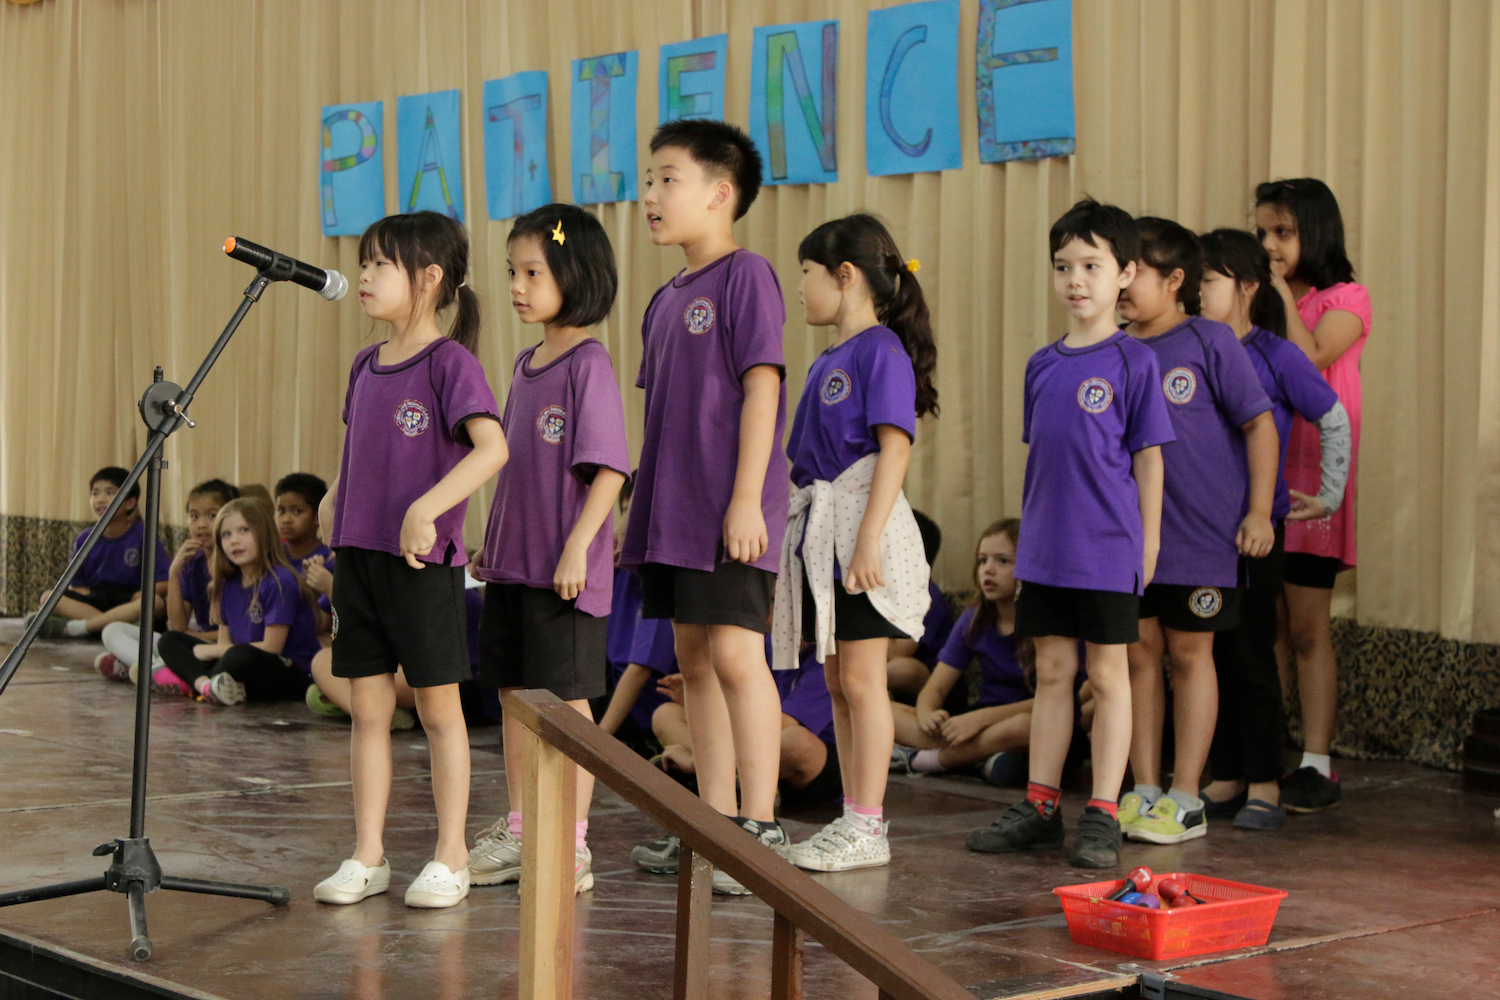
\includegraphics[width=\textwidth]{4_1_1_b.jpg}}

CMIS stakeholders strive to continuously uphold the mission of providing educational excellence, in a caring Christian community that celebrates and respects diversity. \href{https://docs.google.com/a/cmis.ac.th/presentation/d/1EJ3zT-xwUj2W--v5mTN6xWOqewtvhXrhTxXuoR1HyAg/edit?usp=sharing}{CMIS Mission Statement Project} 

The current version of our mission statement resulted from the work of a committee of board members, administrators, teachers, and parents in 2014-2015. Though recently updated, the CMIS mission is still aligned to the historical values of the school.

This year, our student learner outcomes posters displayed around campus were designed and created by our grade 6-12 students. Who We Are Student Poster Competition 

\minor{So what...}

CMIS has a clear Vision, Mission and Student Learner Outcomes that reflect the overall goal of the school community. These are continuously referred to and well known throughout the community. 

We need to find more opportunities to receive feedback from parents on the relevancy of our school “purpose” so we can remain confident that it reflects the beliefs and philosophy of the whole school and its constituency.
\end{findings}

\subsubsection{Purpose, Schoolwide Learner Outcomes, and Profile Data}

\indicator{The student/community profile data and identified global competencies have impacted the development of the school’s vision, mission, and schoolwide learner outcomes.}

\prompt{Evaluate the degree to which the development of the school’s vision, mission, and schoolwide learner outcomes have been impacted by pertinent student/community profile data and identified global competencies, and current educational research}

\begin{findings}
Our community profile data has greatly impacted the development of the\href{http://cmis.ac.th/about/vision}{ CMIS’ Mission, Vision and Student Learning Outcomes Statement}:

{\centering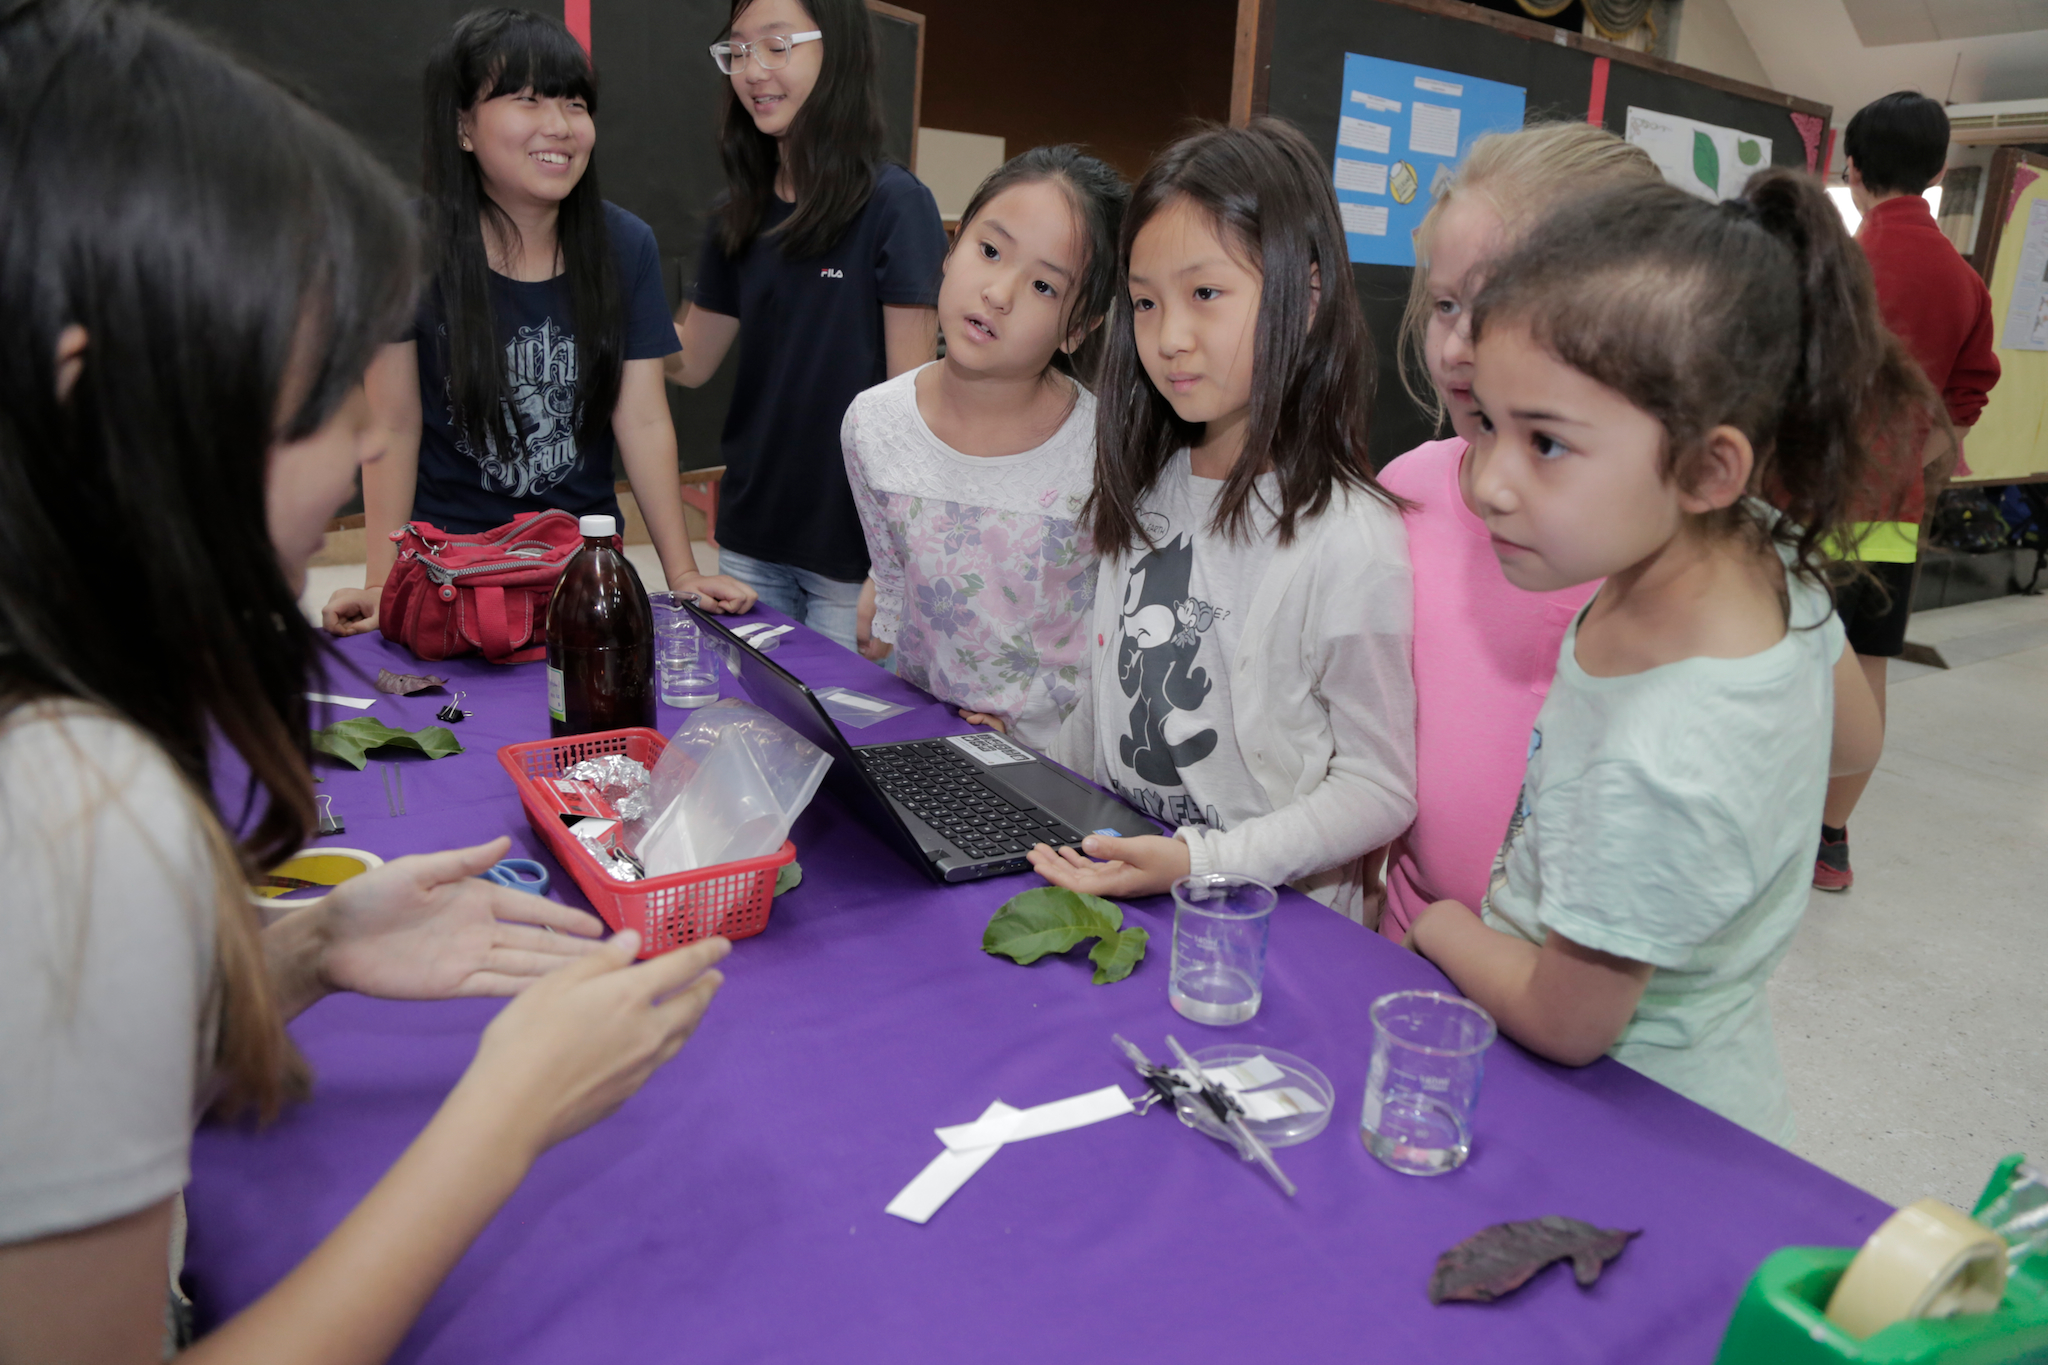
\includegraphics[width=\textwidth]{4_1_1_c.jpg}}

Our \href{https://docs.google.com/document/d/1bIbV9pgGz2vpXYJdnRzL_Od5PS35egy7lgBOBuszgD4/edit}{Student Learner Outcomes} (SLOs) were modified from their original format as Educational Objectives in 2015 to better recognize our diverse student population (32 different nationalities), embrace our global citizenship responsibilities, and include updated 21st century skills. These outcomes were reviewed with all students at the beginning of the 2016-2017 school year and their interpretations were displayed as posters across campus. \href{https://docs.google.com/a/cmis.ac.th/presentation/d/1bdi1LZUjWbGKOyB0XR9CGyoY2xLY39SZVKhiHTIJGxc/edit?usp=sharing}{Student Poster Competition}.

Our diverse group of \href{http://www.cmis.ac.th/about/faculty}{highly qualified educators} originating from over 12 different countries reflect the different cultures and nationalities of our community. Our additional support staff positions also reflect our efforts to meet our community needs (examples: Korean liaison and student spiritual advisor).

CMIS addresses global competencies in a variety of ways beyond the school mission and SLOs. Academically, CMIS students are engaged in learning standards that are internationally benchmarked and rigorous. \href{https://drive.google.com/drive/folders/0ByVFfrm0zfolMVRQYmI1aGlRNDQ}{CMIS Teaching Standards K-12}.

CMIS students have multiple opportunities to engage in school activities and events that require global understanding (e.g. \href{http://gallery.cmis.ac.th/zp-core/full-image.php?a=2010-2011/thai-day-2011/website&i=_mg_3802-version-2.jpg&q=100&wmk=\%21&dsp=Protected\%20view&check=788a1e55c231186711f8dcc0876f4efd0daa0880}{Thai Day}) celebration of diversity (\href{http://gallery.cmis.ac.th/zp-core/full-image.php?a=2013-2014/international_day&i=_MG_6129.jpg&q=100&wmk=\%21&dsp=Protected\%20view&check=788a1e55c231186711f8dcc0876f4efd0daa0880}{International Day}) sharing multiple perspectives (e.g. \href{https://www.nhd.org/}{National History Day}) and using multilingual skills (e.g. Model United Nations Club). 

{\centering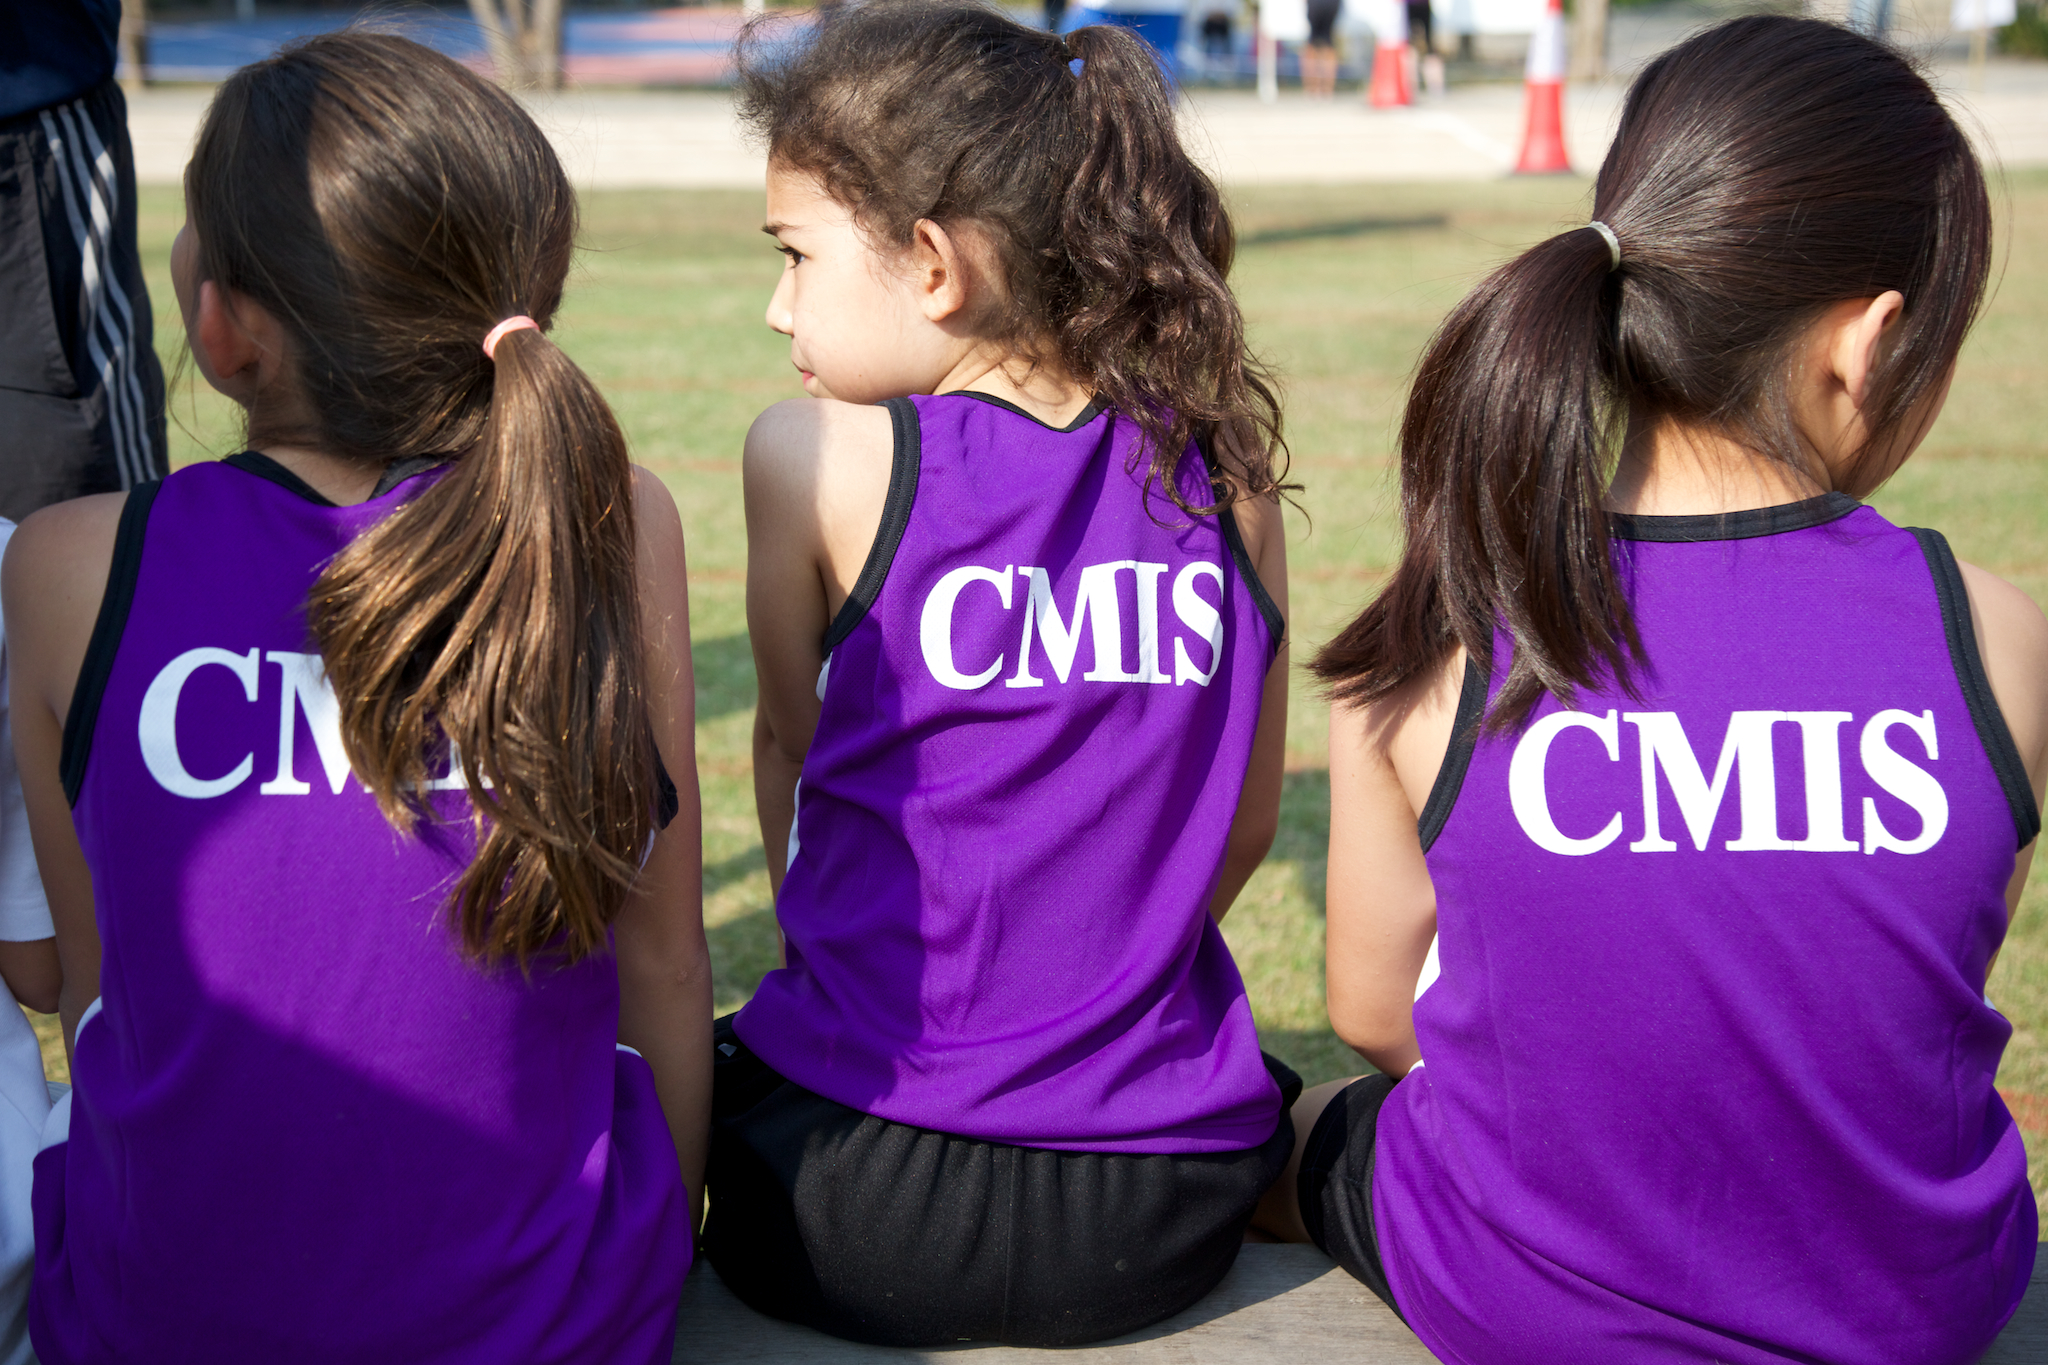
\includegraphics[width=\textwidth]{4_1_1_a.jpg}}

We use globally recognized, research-based standardized tests to identify and assess student needs (e.g, DRA, MAPS, PSAT, and SAT). 

CMIS extracurricular activities (Student Life Beyond The Classroom) emphasize the development of critical thinking skills, the ability to solve problems, and the utilization of effective communication skills. \href{http://blogs.cmis.ac.th/eagles/}{Student Life Beyond the Classroom}

CMIS students participate in community service projects at all three divisions (ES, MS and HS) to promote responsibly in action and service to improve conditions both locally and globally. Examples include Elementary School Thanksgiving Drive for Hope House (local orphanage), \href{https://drive.google.com/a/cmis.ac.th/file/d/0B7jcj1TRcFEGNEtqR3hUSW5QVHM/view?usp=sharing}{Middle School Activity Day} at Hope House and High School \href{http://blogs.cmis.ac.th/community-service/}{community service projects}.

\minor{So what...}

There are many ways in which our school can demonstrate how our vision, mission, and schoolwide learner outcomes have been impacted by pertinent student and community profile data, identified global competencies, and current educational research. 
As our student and community profile is constantly changing, we need to always ensure that we keep abreast of these changes and modify our goals accordingly.
\end{findings}

{\centering
\includegraphics[width=\textwidth]{chapter4_A1.jpg}}

\subsubsection{Involvement of All}

\indicator{The school has a process for involving representatives of the entire school community in the defining of global competencies and in the development/refinement of the core values, mission, vision, and schoolwide learner outcomes.  }

\prompt{Evaluate the processes 1) to ensure the involvement of representatives from the entire school community in the defining of global competencies and the development/refinement of the core values vision, mission, and schoolwide learner outcomes and 2) to determine their effectiveness.}

\begin{findings}
CMIS has several processes for involving representatives of the entire school community in the development/refinement of the core values and schoolwide learner outcomes:

“Teacher Table Talk” sessions are often held during staff development, early release days to capture insights and suggestions about the effectiveness of the CMIS Mission and Student Learner Outcomes.  Example: \href{https://drive.google.com/a/cmis.ac.th/file/d/0ByVFfrm0zfolbHNvSWhVWmJYU3M/view?usp=sharing}{Teacher Table Talk Activity} 

ES students and staff create and participate in monthly \href{https://docs.google.com/a/cmis.ac.th/document/d/1Mv1xjTpbY36naur8SDt9GanKNfR7YtYVL-bWwGLPSHo/edit?usp=sharing}{virtue assemblies} that review and reinforce our school mission, vision and SLO’s. Parents are also invited to attend these events.

{\centering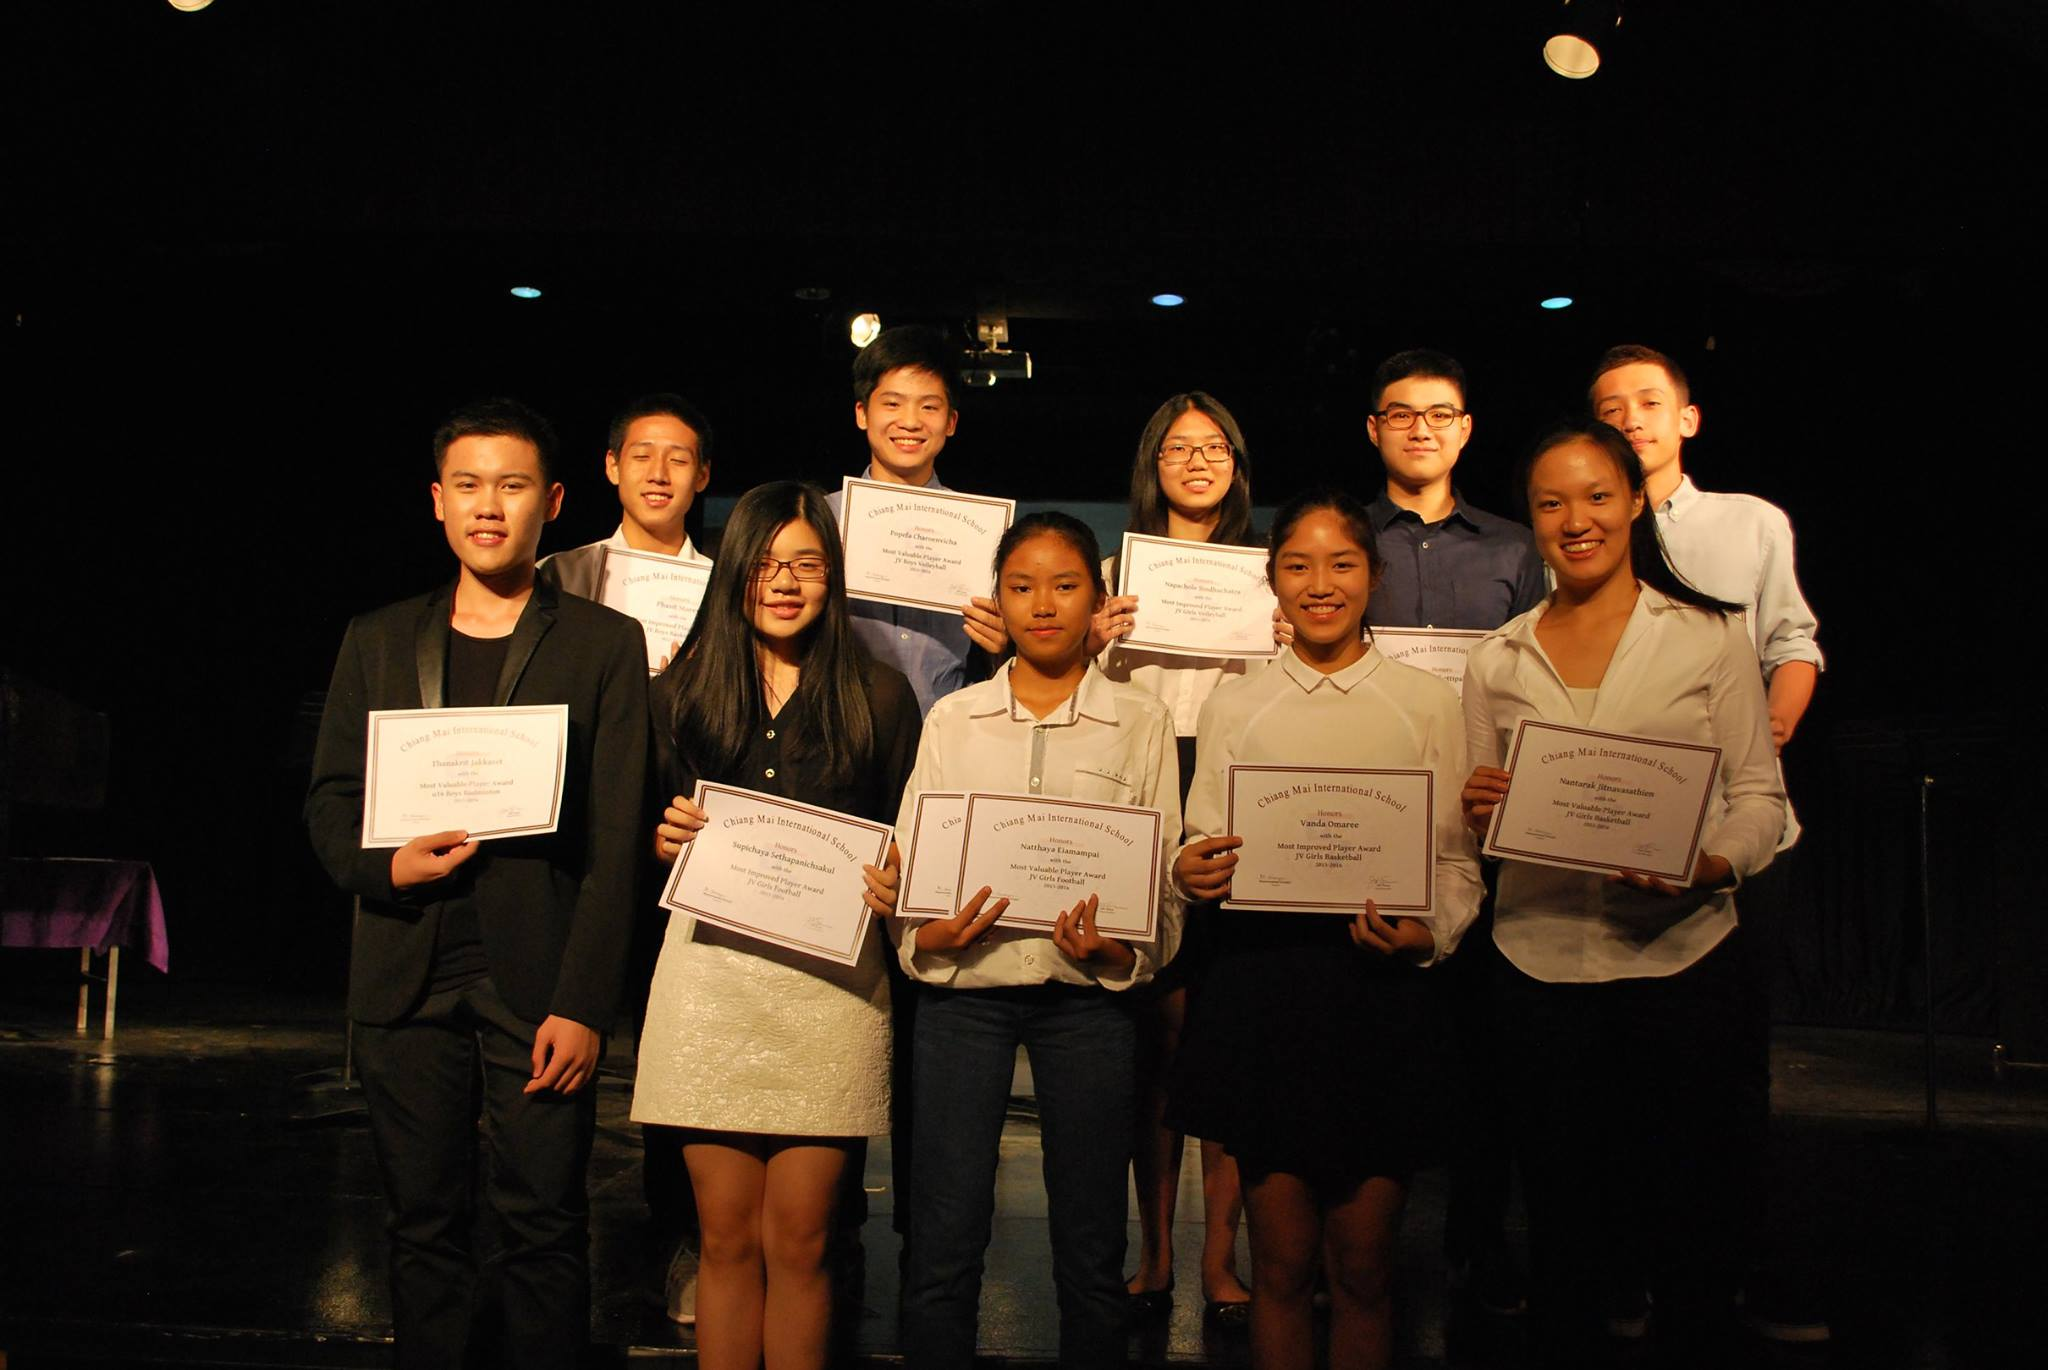
\includegraphics[width=\textwidth]{4_1_1_d.jpg}}

MS and HS Students are encouraged to review our vision, mission, and schoolwide learner outcomes during bi-weekly communication group activities. Communication group have approximately 5-7 students and a teacher leader. This group remains together as a team every year throughout MS and HS.
 
This year, our student learner outcomes posters displayed around campus were designed and created by our grade 6-12 students. \href{https://docs.google.com/a/cmis.ac.th/document/d/1x29XpA7Ro2Xav3JFY0k9F2O22qZi4Yo48hVTYkvhoGM/edit?usp=sharing}{Who We Are Student Poster Competition}.

Several of our student-led clubs involve the defining of global competencies, development/refinement of CMIS core values vision, mission, and schoolwide learner outcomes  (example: CMIS Environmental Club and National Honors Society).

CMIS \href{https://docs.google.com/a/cmis.ac.th/forms/d/16Gbd3MzQOXtjjZ2dG460xw5SHG_eohMIKet3lxYUdAY/prefill}{family surveys} are conducted once a year to solicit feedback from staff, students and parents. The survey gathers data to monitor the effectiveness of CMIS in relation to its mission, vision, and SLO’s. The survey data is analyzed, summarized and used to create goals for improvement. These goals are then shared with each constituency group at the beginning of the year and monitored for progress throughout the year. Example: \href{https://docs.google.com/a/cmis.ac.th/document/d/10w_OSr00xntX42ShaPk4PiNu9FjKP2OgA3g6CKjmEFc/edit?usp=sharing}{Student feedback about cafeteria}.

Our \href{http://blogs.cmis.ac.th/ptg/about/}{CMIS Parent Teacher Leadership Team}- assists and supports the school in the development/refinement of the core values, mission, vision, and schoolwide learner outcomes. This team focuses on this role during monthly meetings with the superintendent, as a leadership team, and during monthly parent meetings that the school management team always attends.

\minor{So what...}

CMIS strives to involve representatives of the entire school community in the development/refinement of the core values and schoolwide learner outcomes.

We believe that we can seek further involvement, and we are trying to reach out and include more involvement with our community-outside of our immediate parent group (examples of progress: reaching out to rotary club and US Consulate).
\end{findings}

\subsubsection{Consistency of Purpose, Schoolwide Learner Outcomes, and Program}

\indicator{There is a strong degree of consistency between the school core values, vision, mission, the schoolwide learner outcomes, and the school program that reflects the school’s explanation of global competencies.}

\prompt{Provide a range of examples that the school vision, mission, schoolwide learner outcomes, and program are consistent. with the school’s explanation of global competencies.}

\begin{findings}
CMIS believes that a global competency doesn't always have to be about world events or other countries, but rather about how to live in the world. Learning how to listen, how to disagree respectfully, how to encourage, and how to collaborate are several elements of a global education that all students need.

The CMIS \href{http://cmis.ac.th/about/vision}{Mission Statement}, \href{http://cmis.ac.th/about/vision}{Student Learner Outcomes}, and school programs are closely related to our goal to equip international students for lives of learning and positive contributions both locally and globally (See \href{http://cmis.ac.th/about/vision}{Who We Are} on website).

CMIS adopted K-12 standards in 2013 that are closely aligned with the school’s mission of academic excellence through rigor, coherence and focus. Our instruction is inquiry-based, which also supports the CMIS key learner outcomes for our students. 

Our grade 6-12 initiative of the 1:1 chromebook reflects our mission to enhance student global proficiency through hands-on, student-centered, and meaningful technology integration. 

Our 2016 \href{https://docs.google.com/a/cmis.ac.th/presentation/d/1xmLAJD96klLrjiBPwCoOMoKmbclYqpIMWaifytzFMgk/edit?usp=sharing}{chromebook survey} results indicated that 73\% of our students felt that the chromebooks increased their ability to demonstrate their learning and 77\% felt that the chromebooks helped them to be more productive. The survey also confirmed how the chromebooks were being used to support essential global competency skills (e,g, presenting, communicating, organizing, researching, and collaborating)

The results of our \href{https://drive.google.com/a/cmis.ac.th/file/d/0B71_pYxcTLo-RlZxQzQyc0NqUFU/view?usp=sharing}{community surveys} confirm that 95\% of our parents parents believe that CMIS provides a high quality education: educational excellence in a caring Christian community that respects and celebrates diversity.

CMIS believes that a global education is not a separate subject or a single lesson; it is a necessary part of all education, for all people. Global education allows a shift in perspective, which provides opportunities for both students and teachers to grow and develop as humans equipped with an understanding of their roles in a complex world.

Some specific teams and staff positions in place to help ensure the promotion of global competency:

\begin{itemize}
\item \href{http://blogs.cmis.ac.th/eagles/}{Student Life Beyond the Classroom} Team
\item Spiritual and Community Service Advisor
\item Spiritual Life Committee
\item \href{http://blogs.cmis.ac.th/ptg/about/}{Parent Teacher Group} Leadership Team
\item Middle School and High School Communication Groups
\item Elementary, Middle, and High School Counselors
\item ES, MS, and HS Student Success Team
\end{itemize}

\minor{So what...}

We have a strong degree of consistency between the school core values, vision, mission, the schoolwide learner outcomes, and the school programs that reflects the school’s explanation of global competencies.

We are trying to move away from the commercial definition of global competency and move towards a more student-centered definition that focuses on authentic opportunities for our community to grow together in a caring community as proactive human beings (i.e. \href{https://drive.google.com/a/cmis.ac.th/file/d/0B0TYmzaZNi3fOF9RQkRqLV9saUE/view?usp=sharing}{Great Kindness Challenge Week}).
\end{findings}

\subsubsection{Communication about Vision, Mission, and Schoolwide Learner Outcomes}

\indicator{The school has means to publicize the \href{http://cmis.ac.th/about/vision}{vision, mission, and schoolwide learner outcomes} to the students, parents, and other members of the school community.}

\prompt{Examine the effectiveness of the means to publicize the purpose and the schoolwide learner outcomes to the students, parents, and other members of the school community.}

\begin{findings}
CMIS has various means to communicate its Vision, Mission Statement and the Student Learner Outcomes to the entire school community:

The CMIS Student Handbook, part of the annual Student Planner, contains information that focuses on our school mission to develop learners who can pursue personal and academic goals, based on academic excellence and strong moral foundations. Link to \href{https://docs.google.com/document/d/1bIbV9pgGz2vpXYJdnRzL_Od5PS35egy7lgBOBuszgD4/edit}{Student Handbook}

Our Vision, Mission and Student Learner Outcomes are displayed prominently throughout campus (examples: student posters and Bible verse banners). 

CMIS publicizes the school vision, mission and student learner outcomes through the CMIS website, accessible to the public and a portal accessible to all parents, students and faculty. It is also included as a footer on all administrative e-mails.  Link to \href{http://cmis.ac.th/about/vision}{Who We Are} on website

School administration always reiterates the school philosophy at all school wide events (e.g. new family orientation, back-to-school night, assemblies). 

As a Christian school, we provide a variety of schoolwide and volunteer opportunities for our community to interact with the Christian ethos, while also respecting the religious diversity of our community (e.g. school-wide Christmas and Easter assemblies, lunchtime bible study groups, and Christian Club Picnic).

Our PTG team reinforces the school vision, mission and student learner outcomes throughout their coffee morning meetings for new families at the beginning of each school year. 

Our board of directors uses the vision and mission in their agenda planning template and uses it as a point of reference throughout their monthly meetings. These meetings are then \href{http://blogs.cmis.ac.th/ptg/public-board-minutes/}{summarized} and shared with our CMIS community on our website.

Our school management team regularly asks for feedback on the effectiveness of our school goals with parents at our PTG meetings, with our staff during our monthly professional development and divisional meetings.

We reflect upon our school goals with our grade 6-12 students during their bi-weekly communications groups and with our elementary students during their and monthly virtue assemblies.

Our teacher leadership team utilize the \href{https://drive.google.com/a/cmis.ac.th/file/d/0ByVFfrm0zfolT25VTjZZRzlXQjA/view?usp=sharing}{meeting wise agenda format} that requires participants to reflect on the objectives of the department meeting in relation to our school goals.

In September a \href{https://docs.google.com/a/cmis.ac.th/presentation/d/1bdi1LZUjWbGKOyB0XR9CGyoY2xLY39SZVKhiHTIJGxc/edit?usp=sharing}{student art competition} was initiated and the student illustration entries were used to better communicate the CMIS vision, mission and student learner outcomes.

Our CMIS weekly newsletter, blogs and \href{https://www.facebook.com/cmis.th/}{Facebook updates} are other effective ways we communicate our Vision, Mission, and Student Learner Outcomes to our community. 

\minor{So what...}

We work hard to publicize the vision, mission, and schoolwide learner outcomes to the students, parents, and other members of our school community.

We are trying to think of more ways of communicating our message in an easier to understand format. Having our students illustrate our philosophy has been very useful, especially with our community members whose english is not their first language.
\end{findings}

\subsubsection{Regular Review/Revision}

\indicator{The school has a process for regular review/revision of the school’s vision, mission, and  schoolwide learner outcomes based on current and future learner needs and other local and global trends and conditions.}

\prompt{Evaluate the effectiveness of the regular process for review/revision of the core beliefs, school vision, mission, and the schoolwide learner outcomes. Include the degree to which the review/revision process addresses current and future learner needs and other local and global trends and conditions.}

\begin{findings}
CMIS has a process for regular review of the CMIS core beliefs based on student needs, global, local needs, and other trends and community conditions.

Our school mission was updated in 2014 and the modified version was formulated by our staff based on current students needs, global and local needs, and other trends and community condition. 

Our Student Learner Outcomes were modified from their original format as Educational Objectives in 2015 to better recognize our diverse community, further embrace students future needs, and include updated global skills. These outcomes were reviewed with the whole community at the beginning of the 2016-2017 school year and student interpretations were displayed as posters across campus. \href{https://docs.google.com/a/cmis.ac.th/presentation/d/1bdi1LZUjWbGKOyB0XR9CGyoY2xLY39SZVKhiHTIJGxc/edit?usp=sharing}{Student Poster Competition}

Each year, CMIS sends an annual community survey (parents, teachers, and students grades 4-12) to solicit perception data related to our effectiveness of implementing our school mission and student learner outcome goals.

\minor{So what...}

As the school’s mission statement and SLOs were recently updated, there has not yet been any rigorous effort to revise them.  However, as CMIS continues to grow and identify innovative ways to enhance teaching and learning, the statement and the SLO’s will be re-evaluated and revised to mirror the diverse needs of our CMIS community.

The CMIS Board has been developing an evaluation instrument for administrators and board members to ensure fidelity to mission, vision, and schoolwide learner outcomes.  Concurrently, the CMIS Board is currently identifying indicators to determine the academic quality and fiscal health of the school. 
\end{findings}

\subsubsection{Conclusions}

\prompt{Comment on the degree to which this criterion is being addressed.}

\begin{findings}

The findings suggest that CMIS addresses this criterion to a high degree. In an effort to increase student achievement further in this area CMIS plans to:

\minor{Maintain and Monitor}

\begin{itemize}
\item Processes and policies that have a strong degree of consistency between the school core values, vision, mission, and the schoolwide learner outcomes.
\item Regular opportunities to continuously communicate school goals with the community
\end{itemize}

\minor{Investigate Better Practice}

\begin{itemize}
\item Ways to communicate CMIS goals in easy to comprehend formats
\item Keeping current with community profile and modifying CMIS goals accordingly.
\end{itemize}

\end{findings}


\subsection{A2 Governance}

The governing authority (a) adopts policies which are consistent with the school’s mission and vision and support the achievement of the schoolwide learner outcomes, i.e., global competencies, (b) delegates implementation of these policies to the professional staff, and (c) monitors results.

\subsubsection{Clear Policies and Procedures}

\indicator{There are clear policies and procedures with regard to the selection, composition, and specific duties of the governing authority.}

\prompt{Evaluate the clarity of the policies and procedures regarding the selection, composition, and specific duties of the governing authority.}

\begin{findings}
The CMIS Board of Directors (the board) has developed clear policies with regard to the selection, composition, and specific duties of the governing authority. 

The board is composed of nine members: four are appointed by the Church of Christ in Thailand (CCT) - our parent organization, three through their role at the school (Director, Manager, Superintendent), one teacher representative, and one parent representative. The teacher representative is elected by the staff and it is preferred (not required) that they serve in a school leadership role (e.g., team leader). They serve for a minimum of two years.

The PTG representative is elected through a process, described further in the \href{http://blogs.cmis.ac.th/ptg/bylaws/}{PTG Bylaws} and serves for a minimum of two years.

Board member roles and responsibilities are clearly outlined and described in the Policies and Procedures Handbook for Administration of the Institutions in the Church of Christ in Thailand

In order to remain current in professional practice, the CMIS Board invited outside consultant John Ritter in September, 2015 to facilitate the discussions on future decisions and outcomes. At this time, the board engaged in a review of its annual goals and the review resulted in a reflection of the school's strengths, weaknesses, threats, and opportunities. 

The board revisited these responsibilities in November 2016 and created a document entitled:  \href{https://docs.google.com/document/d/1EyIeD5g0RDANtZzH5rsCkvDp5ea_bQ2G9rWnhz4QbSc/edit?ts=5881d18d}{Principles of Good Practice}  to better align the board’s responsibilities with the school’s mission, vision, and to further support the achievement of the schoolwide learner outcomes. They also drafted a policy outlining individual board member responsibilities and duties: \href{https://docs.google.com/document/d/14e90Qr4edga9mEZuHIclWeraZ5jgq052IUwcnxTHQZw/edit?ts=5881b471}{Individual Board Member Principles of Good Practice}. These items will be finalized by the board and voted upon for adoption in the February 2017 board meeting.

The board is currently studying the the National Association of International Schools Trustee Handbook (\href{http://www.nais.org/Articles/Pages/NAIS-Trustee-Handbook-Resources.aspx}{NAIS}) together, and using it as a reference for creating future board development.

The board is currently creating a CMIS Board Handbook which is scheduled for compilation by September 2017. This initial version will used as a reference tool for future policies and procedures with regard to the selection, composition, and specific duties of the governing authority. 

\minor{So what...}

The board has focused strongly on adopting policies which are consistent with the school’s mission, vision, and support the achievement of the schoolwide learner outcomes.

Completing the CMIS Board Handbook will allow the BOD to identify additional ways to improve in this area and help to find effective means to communicate these out to our community.
\end{findings}

\subsubsection{Pretraining of Potential Board Members}

\indicator{Individuals who seek board membership or are being considered as appointees by the board will have some form of training in the principles and skills essential to the effectiveness of the school board.}

\prompt{Evaluate the effectiveness of the training that is offered to prospective or new school board members.}

\begin{findings}
CMIS became an official member of the \href{http://www.nais.org/Articles/Pages/NAIS-Trustee-Handbook-Resources.aspx}{National Association of Independent Schools} in 2016 in order to access the most recent research and trends on school governance. 

New CMIS Board members are given a copy of the “International Trustee Handbook of School Board Leaders” to prepare them for their initial tasks of being a CMIS Board member. 

Currently, the CMIS Board utilizes an informal mentoring system where new board members are provided insight and guidance through informal discussions from other senior board members. 

The board chair and newly appointed Superintendent are currently completing book studies together of \textit{Living From the Heart Jesus Gave You} and textit{Joy Starts Here}.Their studies review the Christian ethos, how it relates their own personal journey in Christianity and the Christian vision for CMIS. This mentorship relationship highlights the importance of a strong partnership between the chair and the head of the school,

``It is critical that the chair and head make every effort to establish a solid and mutually supportive relationship based on respect and trust, develop the capacity to be forthright and candid, and listen to and learn from each other's feedback. The board chair and the head share the same goal: providing effective leadership for the school.'' \textit{NAIS Trustee Handbook} p.125

Current and prospective board members have attended EARCOS workshops together for the past two years. Sessions attended by board member at the 2015 EARCOS Leadership Conferences:
\begin{itemize}
\item Learning from Lincoln Leadership
\item Strategic Planning for Effective School Boards 
\item Parent Teacher Organizations: Effective Communication
\item Effective Adoption and Resource Cycles 
\end{itemize}

All board members were asked to review and sign \href{https://docs.google.com/a/cmis.ac.th/document/d/1sVjFjeVtwbk0-n8GsM5K_XzZSn2wejtlJ3kurXUrKGU/edit?usp=sharing}{CMIS Board of Directors: Roles and Responsibilities} of the \href{https://docs.google.com/a/cmis.ac.th/document/d/1sVjFjeVtwbk0-n8GsM5K_XzZSn2wejtlJ3kurXUrKGU/edit?usp=sharing}{Board and CMIS BOD Code of Conduct} at the beginning of the 2016-2017 school year.

\minor{So what...}

The CMIS Board of Directors has worked hard to increase the pre-training and support for new board members but acknowledges that it can do more. The CMIS Board Handbook will include further strategies for new BOD training and support.
\end{findings}

{\centering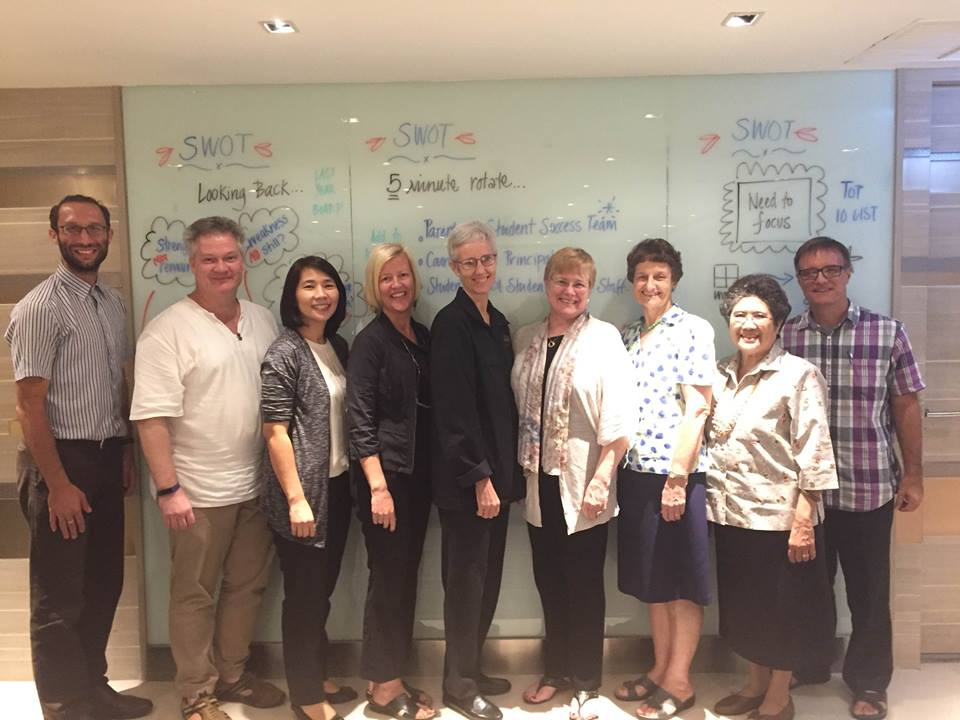
\includegraphics[width=\textwidth]{chapter4_A2.jpg}}

\subsubsection{Relationship of Policies}

\indicator{The governing authority’s policies are directly connected to the school’s vision, mission and schoolwide learner outcomes that focus on student achievement of global competencies.}

\prompt{Evaluate the adequacy of the policies to support the school’s vision, mission, and schoolwide learner outcomes through its programs and operations.}

\begin{findings}
The CMIS Board models collaborative leadership that provides a unified direction to all leaders and members of the staff. This direction is clearly connected to the school’s purpose evident in its vision, mission, and \href{https://docs.google.com/document/d/1bIbV9pgGz2vpXYJdnRzL_Od5PS35egy7lgBOBuszgD4/edit}{student learner outcomes} (SLOs).

The effective involvement of all stakeholders, starting from the governing authority, in formulating and implementing the vision, mission, and SLOs, ensures that student achievement is the focus of all school decisions. The guidance and leadership of the governing authority provide the momentum necessary to effectively address our vision, mission, and SLOs.

The CMIS Board is responsible for providing the necessary learning programs and operations that support CMIS curriculum and resources, attracting and retaining quality employees, and ensuring the availability of learning materials and supplies. Through the budget funding process, the board also supports professional development for teachers, administrators, support staff, and the board.

At a summer 2016 Board Retreat, the current CMIS Board created a plan for areas of improvement that are based on the following topics: 

\begin{itemize}
\item Stakeholder communications
\item Funds development
\item Strategic planning
\item board handbook
\end{itemize}

The board also developed strategies and procedures to address these areas and are in the process of developing measurable goals to evaluate the effectiveness of these actions. The goals focus on the board’s responsibility to be good stewards of its resources, its fiduciary responsibilities, and on providing clear, strategic leadership to ensure CMIS is viable for years to come.

The CMIS mission, vision, and SLO are consistently integrated into the board agenda template. This is done to ground the meeting in the important work of school outcomes and focus members on our students and their achievement. 

\minor{So what}

CMIS acknowledges that the past decisions and proposals of the board have often been recorded in board minutes that can be difficult to locate and refine. This limits the current board’s ability to effectively evaluate the connectedness of CMIS Board practices, in relation to the the school’s vision and mission.

In an effort to address this challenge, the board has appointed a committee to facilitate the creation of a CMIS Board Handbook, which is scheduled for compilation by September 2017. This Handbook will make it easier for evaluation as the policies will be created in a common format and available in a central location. 
\end{findings}

\subsubsection{Involvement of Governing Authority}

\indicator{The governing authority is involved in the regular review and refinement of the school’s vision, mission, and schoolwide learner outcomes. The governing authority uses a variety of strategies to remain current in research-based knowledge about effective schools.}

\prompt{Evaluate the processes for the involvement of the governing board in the regular review and refinement of the school’s vision, mission, and schoolwide learner outcomes.}

\begin{findings}

The governing authority is involved in the regular review and refinement of the school’s \href{http://cmis.ac.th/about/vision}{vision, mission, and schoolwide learner outcomes}. It also uses a variety of strategies to remain current in research-based knowledge about effective schools.

As mandated by the ``Board of Directors Roles and Responsibilities of the Board'', the board reviews the mission, vision, and schoolwide learner outcomes at the beginning of each school year. For example, in May 2014 the board voted to revise the vision and mission statement, and in 2015 voted to revise the schoolwide learner outcomes so they were more measurable and in line with the Focus on Learning recommendations. 

In order to remain current in research based knowledge about effective schools, the CMIS Board invited outside consultant John Ritter in September, 2015 to facilitate board development  that reviewed the characteristics of effective school boards. In summary, the workshop focused on:

\begin{itemize}
\item Having a shared vision about high capabilities of both students and staff
\item Being policy and accountability driven
\item Engaging in goal-setting processes that can drive action in the school to improve
\item Aligning resources around those goals
\item Using data to diagnose problems and to monitor and drive continuous improvement efforts
\item Communicating and engaging with the community
\item Working well together as a team 
\end{itemize}

These characteristics have been used as the foundation for CMIS Board planning and will provide the framework of the CMIS Board Handbook. The board chair also studied the book, \href{https://www.amazon.com/Governance-Leadership-Reframing-Nonprofit-boards/dp/0471684201}{\textit{Governance as Leadership}}  which reviews the process of generative thinking in relation to strategic planning and plans to also use the guidelines from this research based book in the compilation of the CMIS Board Handbook.

CMIS is a member of The International School Association of Thailand (ISAT). ISAT works with government ministries to keep current of the benefits of international education in Thailand and promotes quality international school education.

The quality of education offered at the ISAT member schools has been recognized by accreditation organizations such as the \href{https://en.wikipedia.org/wiki/Western_Association_of_Schools_and_Colleges}{Western Association of Schools and Colleges} (WASC), and the \href{https://en.wikipedia.org/w/index.php?title=Council_of_International_Schools&action=edit&redlink=1}{Council of International Schools} (CIS).

The CMIS Superintendent and Manager serve on the CMIS Board and attend the \href{https://drive.google.com/a/cmis.ac.th/file/d/0Bwny3HLdIIS7LUtqTlR2REhsLVBkWHVib3k3V1hsWVFtUzIw/view?usp=sharing}{ISAT quarterly meetings} together. It is a great opportunity to review the CMIS vision, mission, and schoolwide learner outcomes in relation to other schools in Thailand. 

At the ISAT meetings there are often guest speakers (e.g., in November, Dr. Chaipreuk Sereerak, Permanent Secretary, Ministry of Education and Mr. Krittachai Aroonrat, Secretary General, Office of Private Education Commission) . Their expertise and guidance assist the board in remaining current about effective schools international school policy and educational trends in Thailand (\href{http://www.isat.or.th/members/announcement-updates/minutes-isat-general-member-meeting-22016}{sample minutes}).

CMIS Manager, \href{https://drive.google.com/a/cmis.ac.th/file/d/0Bwo-i12FeO0rY1V1SGtuSzJBd1U/view?usp=sharing}{Patcharin Jingkaojai} was elected in 2016 to the ISAT Management Committee which provides leadership and support to membership schools throughout Thailand. In September 2016 the Management Committee organized the \href{https://drive.google.com/a/cmis.ac.th/file/d/0Bwo-i12FeO0rQ0JOZ09JVTNEUTA/view?usp=sharing}{Regional Member Meeting} that was hosted at CMIS. 

In 2016, the CMIS Superintendent, Nel Capadona joined the ISAT Professional Development Committee and assists with supporting professional development, school development, and networking for ISAT member schools. In November 2016 they promoted the \href{https://drive.google.com/a/cmis.ac.th/file/d/0ByVFfrm0zfolSXFEZFJVN1VOaTQ/view?usp=sharing}{EARCOS Focus, Coherence and Rigor Math Workshop} that was hosted by CMIS.

\minor{So what...}

The CMIS BOD works hard to regularly review and refine the school’s vision, mission, and schoolwide learner outcomes. 

The board is currently completing a book study together of the \textit{International Trustee Handbook of School Board} (NAIS). The handbook has been a valuable resource on reflecting upon how to effectively review and refine school goals. The board plans to complete their own handbook by September 2017 and use it as the foundation for future BOD strategic planning.

\end{findings}

\subsubsection{School Community Understanding}

\indicator{ The school community understands the governing authority’s role.}

\prompt{To what degree does the school community understand the governing authority’s role?}

\begin{findings}
The CMIS Board ensures community understanding of their role through a variety of means. 

The board works hard to adhere to the best practice that, ``An effective board keeps its most important records of business up-to-date and ensures that they are accurate, concise, and timely'' (Devarics, 2011).

For example:

board agendas are planned by the school executive team with the board chair and sent out to all board members a week before the monthly board meeting for review and comment. 

board minutes are kept by the board secretary, approved at the next meeting and summarized for the community on the PTG website. The meeting summaries are also referenced by the superintendent at the monthly PTG meetings. \href{http://blogs.cmis.ac.th/ptg/public-board-minutes/}{Public board minutes on PTG Blog}

Currently, the CMIS Board is developing a CMIS Board Handbook to ensure a clearer understanding of the relationship between the governing authority and the community. The board is using the National Association of International Schools (\href{http://www.nais.org/Articles/Pages/NAIS-Trustee-Handbook-Resources.aspx}{NAIS}) Trustee Handbook as a research based reference for this project: Chojnacki, David. \href{https://www.nais.org/Bookstore/Pages/ProductDetail.aspx?productid=\%7B47CD9104-BC67-E111-9A8C-00505683000D\%7D}{INTERNATIONAL Trustee Handbook: A Guide for Effective Governance for Independent School Boards}. 

Though the board clearly understands the limits of the board/community relationship, the CMIS Board is working hard to increase opportunities to formally and informally interact with the community to ensure that, “...the school is fulfilling its mission with vision and energy, [and that] all  of the school’s constituents will be bound together by this mission (NAIS Trustee Handbook, Chojnacki, 139)  

Examples:

Formal opportunities to interaction with Parents include:
\begin{itemize}
\item board members attend parent \href{https://drive.google.com/a/cmis.ac.th/file/d/0Bwny3HLdIIS7d1FGeDhaZE1EcG1PMHlMX2NRZTdIYXlWZERB/view?usp=sharing}{coffee mornings} at start of the school year
\item board members attend and speak at \href{https://drive.google.com/a/cmis.ac.th/file/d/0Bwny3HLdIIS7NGpoVEtlWmw2RE0/view?usp=sharing}{Senior Graduation day}
\item board members welcome at New Family Orientation Day
\end{itemize}

Informal opportunities to interact with Parents include:
\begin{itemize}
\item board members attend monthly PTG Meetings
\item board members sponsoring student organizations (e.g. \href{https://drive.google.com/a/cmis.ac.th/file/d/0Bwny3HLdIIS7WXpial9KYjFlWFBBQW1YQ2thOVpsTTFCeGVr/view?usp=sharing}{Boy Scouts})
\item board members mingle with families during Welcome Back BBQ
\item board members attend Social school events (Latin Night, CMIS Invitational Basketball Tournament, etc.)
\end{itemize}


Recent CMIS \href{https://docs.google.com/a/cmis.ac.th/document/d/1_otvw47y3Z-1CSjXnKhgRTauVRqPl1S6nSdmsb00O2k/edit?usp=sharing}{family survey results} indicate that the majority of our community believe that the CMIS Board communicates effectively with the community and that our ratings have increased in this area over the last two years.

This year, in an effort to increase the board's communication efforts further CMIS has included photos and provided backgrounds of our board members and their board roles on our school website. We have generated \href{https://drive.google.com/a/cmis.ac.th/file/d/0Bwny3HLdIIS7MjJMX1ZIVS1zSXJOaTNZcFRmTWV1Q1VTc1hZ/view?usp=sharing}{annual community letters} from the board chair and our School Executive Team updating the community of our current goals and our appreciation for their support.

\minor{So what...}

The board has devoted time and resources to improve in this area but there is always room for additional communication. They plan to do this by:

Including more specific questions about the board’s effectiveness in next year’s community survey. 

Changing the response format to make data analysis easier to correlate and manipulate. The current ``neutral'' option makes responses difficult to interpret.
\end{findings}

\subsubsection{Relationship to Professional Staff}

\indicator{There is clear understanding about the relationship between the governing authority and the responsibilities of the professional staff. The governing authority limits its actions to policy making and strategic planning — authorizing the administration to implement its decisions.}

\prompt{Determine whether there is clear understanding about the relationship between the governing board and the responsibilities of the professional staff and how that understanding is developed and maintained.}

\begin{findings}
\href{https://docs.google.com/a/cmis.ac.th/document/d/1_otvw47y3Z-1CSjXnKhgRTauVRqPl1S6nSdmsb00O2k/edit?usp=sharing}{Data} indicates that there is a clear understanding about the relationship between the governing board and the responsibilities of the professional staff and how that understanding is maintained. 

During the 2016-2017 Board Retreat the board reviewed the Board of Directors Roles and Responsibilities and The Board Code of Conduct. These documents clearly define the board responsibilities in relation to the CMIS staff and community. In an effort to increase understanding these documents have been made available for review on the CMIS website.

Currently, the CMIS Board is developing a CMIS Board Handbook to ensure a clearer understanding of the relationship between the governing authority and the professional staff. The board is using the National Association of International Schools Trustee Handbook as a research based reference for this project: Chojnacki, David (\href{http://www.nais.org/Articles/Pages/NAIS-Trustee-Handbook-Resources.aspx}{NAIS}). \href{https://www.nais.org/Bookstore/Pages/ProductDetail.aspx?productid=\%7B47CD9104-BC67-E111-9A8C-00505683000D\%7D}{INTERNATIONAL Trustee Handbook: A Guide for Effective Governance for Independent School boards}. 

Though the board clearly understands the limits of the board/faculty relationship, the CMIS Board is working hard to increase opportunities to formally and informally interact with faculty to ensure that, “...the school is fulfilling its mission with vision and energy, [and that]  all  of the school’s constituents will be bound together by this mission (NAIS Trustee Handbook, Chojnacki, 139)  

Examples:
Formal opportunities to interact with Administrators and Faculty:
\begin{itemize}
\item board members participating in FOL/WASC focus groups (early release days)
\item board members attending New Teacher Orientation
\item board Chair providing Welcome Back Blessing at beginning of the school year. 
\item board presenting at Teacher Appreciation and Farewell Staff Luncheon 
\item board members leading prayer during school-wide assemblies.
\end{itemize}

Informal opportunities to interact with Administrators and Faculty: 
\begin{itemize}
\item board members attending school fundraisers (e.g., Latin night)
\item board members attending school performances
\item board members attending social and sporting events
\item board members providing spiritual guidance to volunteer staff members
\end{itemize}

\minor{So what...}

The board has worked hard to define the relationship between the governing authority and the responsibilities of the professional staff. The BOD has tried to limit its actions to policy making and strategic planning — authorizing the administration to implement its decisions.
\end{findings}

\subsubsection{board Evaluation/Monitoring Procedures}

\indicator{There is clarity of the evaluation and monitoring procedures carried out by the governing board, including the review of student performance, overall school programs and operations, and the fiscal health of the school.}

\prompt{Determine the degree to which there is clarity of the evaluation and monitoring procedures carried out by the governing board, including review of student performance, overall school programs and operations, and fiscal health of the school.}

\begin{findings}
The board participates in regular evaluation and monitoring procedures, including the review of student performance, overall school programs and operations, and the fiscal health of the school.

The CMIS School Executive Team (\href{https://drive.google.com/a/cmis.ac.th/file/d/0Bwny3HLdIIS7di1mY0xFMnJyWmQzNEhON09EREpvY0JRd0Jv/view?usp=sharing}{Manager, Superintendent, and Director}) present monthly \href{https://docs.google.com/document/d/1gz3SiCiPUMU9n-JgGqzGQhgl0r0qAdpSfQPtBK-rwyI/edit}{SET} reports to the board that include updates on specific elements of school performance, programs, development, operations, and fiscal health. The Superintendent focuses on clarifying admission trends, evaluating academic excellence, demonstrating achievement, reviewing professional development projects, and providing updates on accreditation. The Director focuses on sharing initiatives to ensure compliance with Thai regulations (i.e. ONESQA) and the CCT spiritual growth initiatives (example: \href{http://blogs.cmis.ac.th/spiritual-life/2017/02/03/the-lords-prayer-weekly-devotional-60217-100217/}{The CMIS Lighthouse: Weekly Devotion}). Finally, the Manager ensures that appropriate financial audits are completed for CCT monitoring, and that fiscal procedures and resources are being used with fidelity. 

Beginning in 2015, the board began to send out a \href{https://docs.google.com/a/cmis.ac.th/document/d/16DVRIWxzKBgzVMqk8coHlO97SFWthAA_DEx4z6WSHQs/edit?usp=sharing}{Community Report} that reviews student performance, overall school programs and operations, and the campus development of the school each semester.  

As part of the 2015 and 2016 annual board Retreat, a report and evaluation of student performance, programs, and teacher professional development was part of the board planning for the upcoming year. 

Currently, the CMIS Board is completing a book study together of the research-based (\href{http://www.nais.org/Articles/Pages/NAIS-Trustee-Handbook-Resources.aspx}{NAIS}) Trustee Handbook.  Based upon the findings of this reference tool, one of the 2016-2017 board goals is to communicate this evaluation to our community at the end of this year in the form of a CMIS Annual Report.

\minor{So what...}

Currently, the board implements monitoring and evaluation processes based upon perceptual data only. Though this is useful and helpful data, the board would like to begin collecting more quantitative data to help make governance decisions, such as: student data that is aligned to adopted standards and data that correlates to specific school programs and operations and fiscal health indicators. 
\end{findings}

\subsubsection{Complaint and Conflict Resolution Procedures}

\indicator{The established governing board/school’s complaint and conflict resolution procedures as they apply to the school’s stakeholders are effective.}

\prompt{Comment on the effectiveness of the established governing board/school’s complaint and conflict resolution procedures as they apply to the school’s stakeholders.}

\begin{findings}
CMIS has clear complaint and conflict procedures in place to work through unresolved situations, where an action or decision may be considered unfair or inappropriate.  

There is an anonymous process for teachers to share concerns with administration through the Teacher Administration Communication Team (\href{https://docs.google.com/a/cmis.ac.th/document/d/14nhwcw8xo3i-23Q-WUxo6KJ_c8yFKu-jTdCctt4MFcs/edit?usp=sharing}{TACT}) that meets monthly to review and address current staff concerns. The concerns are addressed collaboratively and a \href{https://docs.google.com/a/cmis.ac.th/document/d/1KLB4c5_LkxXzq4vP2EuNhBVPp2q_FT9qy1cBBwaS5JM/edit?usp=sharing}{summary} of the solutions and suggestions are e-mailed out to all staff.

If teachers have concerns related to their students, they are encouraged to reach out to the Student Success Team facilitated by our Student Service Coordinator.  There is a \href{https://docs.google.com/a/cmis.ac.th/forms/d/e/1FAIpQLScVtFtaEXarGOjwsiJyGdbLAMbeNzG9m44i1fWXFLbtMKZcUg/viewform}{Student Service Request Form} available on the teacher dashboard section of the CMIS website. This form activates immediate support from the divisional counselor to meet with the teacher and create a plan of action.

There is also a formal structure in place with regard to resolving internal conflicts between teachers and administration through the board of directors (\href{https://docs.google.com/a/cmis.ac.th/document/d/1RRBuWgqIb-BlwD8vTRrTG0u_FCHgQFD_oEbvseNdAPc/edit?usp=sharing}{Staff Grievance Policy}). This policy is included in the \href{https://docs.google.com/document/d/1fNreQp5yTOg_g9K4UnR8xvyQf-GcFOHo-6Onp4SqlKg/edit}{CMIS Faculty Handbook}.

Parents with student or school concerns are directed to page 26 of the Student Planner: Communication between School and Home, which contains the process of communicating issues with the school.
Parents are also encouraged to share their concerns or suggestions with the superintendent during the weekly '\href{http://blogs.cmis.ac.th/newsletter/2016/09/05/super-thursdays-starts-this-week/}{Super Thursdays}' or a \href{http://blogs.cmis.ac.th/ptg/about/}{PTG Leadership Team} member at any time. 

\minor{So what...}

The CMIS Board will continue to monitor and maintain the programs and processes that are in good standing. There are areas of growth in this section, for example: the community suggested creating a Sounding Board Session where members from the community (i.e. students, parents, teachers) can meet with the board in an informal setting to discuss concerns and suggestions. CMIS looks forward to piloting this process in March 2017
\end{findings}

\subsubsection{Evaluation Procedures}

\indicator{The governing authority carries out clearly defined evaluation procedures.}

\prompt{Comment on the clarity of the evaluation procedures carried out by the governing authority.}

\begin{findings}
The School Executive Team (Manager, Superintendent, and Director) presents monthly \href{https://docs.google.com/document/d/1gz3SiCiPUMU9n-JgGqzGQhgl0r0qAdpSfQPtBK-rwyI/edit}{School Executive Team Reports} to the board that include updates on specific elements of school performance, programs, professional development, operations, and fiscal health. 

As part of the 2015 and 2016 annual \href{https://drive.google.com/a/cmis.ac.th/file/d/0B-CVlEN-TDChSTJ6QzdQQUczT0k/view?usp=sharing}{Board Retreat}, a Strength, Weakness, Opportunities and Threats (\href{https://drive.google.com/a/cmis.ac.th/file/d/0B-CVlEN-TDChNVJudnJBNnZveTQ/view?usp=sharing}{SWOT}) analysis was completed. The purpose of a SWOT analysis is to identify:

\begin{description}
\item [Strengths] Factors that are likely to have a positive effect on (or be an enabler to) achieving the CMIS objectives.
\item [Weaknesses] Factors that are likely to have a negative effect on (or be a barrier to) achieving CMIS objectives.
\item [Opportunities] External factors that are likely to have a positive effect on achieving or exceeding CMIS objectives, or goals not previously considered.
\item [Threats] External factors and conditions that are likely to have a negative effect on achieving CMIS objectives, or making the the objective redundant or unachievable.
\end{description}

During the 2016 retreat the board also created goals based on feedback from a \href{https://docs.google.com/a/cmis.ac.th/document/d/1QoHZUrC_PbxitA2t_ZGH8DidxTLVe46HSl9otFPnE4k/edit?usp=sharing}{community perception survey} that was studied to evaluate what is effective and less effective CMIS programs, systems and procedures.

Beginning in 2015, the board began to send out \href{https://docs.google.com/a/cmis.ac.th/document/d/16DVRIWxzKBgzVMqk8coHlO97SFWthAA_DEx4z6WSHQs/edit?usp=sharing}{Community Plan Updates} that reviewed student performance, overall school programs and operations, and the fiscal health of the school each semester.  

\minor{So what...}

The CMIS Board has spent time and effort identifying the school’s strengths, weaknesses, opportunities, and threats. This year, the board has developed strategies and processes to maximize the strengths and opportunities and diminish the threats and weaknesses detailed from the SWOT analysis. The board is currently in the process of reviewing the implementation of these strategies. After the review, the board will monitor and maintain those strategies that are effective and modify those that could be improved. These committees are outlined in the section entitled: Relationship of Policies. 
\end{findings}

\subsubsection{Evaluation of Governing Authority}

\indicator{There is a process for evaluating the governing authority.}

\prompt{Review and assess the process for evaluating the governing authority}

\begin{findings}
The board currently uses \href{https://docs.google.com/a/cmis.ac.th/document/d/1_otvw47y3Z-1CSjXnKhgRTauVRqPl1S6nSdmsb00O2k/edit?usp=sharing}{CMIS community survey results} to evaluate the board’s effectiveness as a collective group as well as the Superintendent as a leader. 2016 data indicates that the majority of our parents believe that the CMIS Board and school leadership are effective.

The CMIS Board is currently completing a Due Diligence Checklist based on the guidelines included in the International Trustee Handbook: A Guide for Effective Governance for Independent School Boards (Chojnacki).The checklist will be used to complete an internal evaluation by the board that can be used in conjunction with the family survey results to create meaningful goals for for future board improvement.

The board chair and newly appointed Superintendent are working together to create a comprehensive Superintendent evaluation instrument and process. They plan to present the research based model to the board in April for review and adoption for the 2017-2018 school year.

\minor{So what...}

The board acknowledges that this is an area for future board improvement and that additional data sources should be used for board evaluation. It also realizes that the current community survey format should be modified to increase usefulness. Eliminating the “neutral “ option, preventing questions from being skipped and adding more specific questions related to the boards effectiveness are being implemented in this year’s April survey.
\end{findings}

\subsubsection{Conclusions}
\prompt{Comment on the degree to which this criterion is being addressed.}

\begin{findings}
The findings suggest that CMIS addresses this criterion to a high degree. In an effort to increase student achievement in this area the CMIS Board plans to:

\minor{Maintain and Monitor}
\begin{itemize}
\item Processes and policies that focus on the CMIS Vision, Mission, and Schoolwide Learner Outcomes
\item Compilation of the CMIS Board of Directors Handbook
\item Completion of the NAIS Trustee Handbook board book study
\end{itemize}

\minor{Continue to Improve}

\begin{itemize}
\item Increased communication with stakeholders regarding board roles and CMIS achievement
\end{itemize}

\minor{Investigate Better Practice}

\begin{itemize}
\item To find additional ways to evaluate board effectiveness outside of perceptual data. 
\end{itemize}
\end{findings}

\subsection{A3 School Leadership}
The school leadership (1) makes decisions to facilitate actions that focus the energies of the school on student achievement of the schoolwide learner outcomes, i.e., global competencies, (2) empowers the staff, and (3) encourages commitment, participation, and shared accountability for student learning in a global environment.

\subsubsection{Defined Responsibilities, Practices, etc.}

\indicator{The school has administrator and faculty written policies, charts, and handbooks that define responsibilities, operational practices, decision-making processes, and relationships of leadership and staff.}

\prompt{Evaluate these administrator and faculty written policies, charts, and handbooks. Determine the clarity and understanding of these by administration and faculty.}

\begin{findings}
CMIS has clear policies that define responsibilities, operational practices, decision making processes and relationships of leadership and staff. 

These policies and procedures can be found in the CMIS employment contracts and the \href{https://drive.google.com/a/cmis.ac.th/file/d/0ByVFfrm0zfolVm9uc19UNl82NVpPMUZ1ZEstZlFidEY1c2hn/view?usp=sharing}{CMIS Faculty Handbook}. They are reviewed annually during the administrative, new teacher, and returning staff orientations. 

Furthermore, a list of administrative teams is included in the Faculty Handbook and CMIS Student Planner. 

CMIS organized ``\href{https://drive.google.com/a/cmis.ac.th/file/d/0ByVFfrm0zfolbHNvSWhVWmJYU3M/view?usp=sharing}{Teacher Table Talk}'' sessions during early release days to capture insights and suggestions about the decision-making processes and relationships of leadership and staff. 

In November, 2016 the \href{https://docs.google.com/a/cmis.ac.th/document/d/1iW_tWIwRlWU2p0oIOvd3usDsxj9qYDt_2ROwNPBTHSc/edit?usp=sharing}{Teacher Leadership Team}  which is made up of teachers and administrators, participated in the revision of the handbook format and made it available in an electronic formatted version. We plan to make this an annual project as it was previously revised only by administrators.

CMIS Board governance requires the School Executive Team (i.e. Superintendent, Director and Manager) to maintain up-to-date operational handbooks and procedural guidelines.

Board member roles and responsibilities are clearly outlined and described in the \textit{Christian Churches of Thailand Board Handbook}.

\minor{So what...}

CMIS Leadership has clearly defined roles for teachers only through a variety of methods, most notably the Teacher Handbook. CMIS should continue to maintain, monitor, and modify, as necessary, the Teacher Handbook with stakeholder feedback and input. Additionally, CMIS should develop a Leadership Handbook to clearly outline the roles and responsibilities of principals, directors, and team leaders.
\end{findings}

\subsubsection{Existing Structures}

\indicator{The school has existing structures for internal communication, planning, and conflict resolution.}

\prompt{How effective are the existing structures for internal communication, planning, and conflict resolution?}

\begin{findings}

CMIS has many existing structures for internal communication, planning, and resolving differences.

Communication and Planning Examples:
The School Executive Team (SET) shares information from the monthly Board of Director Meetings to the School Management Team (SMT), and to the \href{https://docs.google.com/a/cmis.ac.th/document/d/1iW_tWIwRlWU2p0oIOvd3usDsxj9qYDt_2ROwNPBTHSc/edit?usp=sharing}{Teacher Team Leaders} who communicate the information to the teachers.

Internal communication is also highlighted through Weekly \href{https://docs.google.com/a/cmis.ac.th/document/d/1Jh_VpJ8rfb4_OwmpRw6VZCrIYAuV6A0SP_3NN82KD7A/edit?usp=sharing}{HS Principal Notes}, MS Principal Message and ES Principal Notes that are sent electronically to all staff.

The Superintendent and principals are out on campus every morning before school for personal communication with students, parents and staff.

The Superintendent and principals meet weekly to address any community concerns and plan.

Additionally, e-mails, memos, google docs are used to further enhance communication.

\minor{Communication Examples}

Internal communication and planning is included at \href{https://docs.google.com/a/cmis.ac.th/document/d/1tSEBD59kwf83Z0-m1Q4hzNrVwaJMHdracrghwqoSdW0/edit?usp=sharing}{monthly staff meetings} are held every Wednesday for K-12 Teams, ES, MS and HS Divisions, Teacher Leadership Teams, and Early Release Professional Development Trainings.

PTG Team Leaders meet with the Superintendent monthly to discuss parent concerns or suggestions for school improvement.

StuCo (Student Council) and the Superintendent meet for lunch each semester to discuss student suggestions and ideas for school improvement.

\minor{Conflict Resolution Examples}

CMIS organizes \href{https://drive.google.com/a/cmis.ac.th/file/d/0ByVFfrm0zfolWUs2RGMxczFXRXRqbDRjRlF2SGQ5cVZfV0FZ/view?usp=sharing}{Teacher Table Talk} sessions during early release days to capture insights and suggestions about the existing structures for resolving differences.

There is an anonymous process for teachers to share concerns with administration through the Teacher Administration Communication Team (\href{https://docs.google.com/a/cmis.ac.th/document/d/14nhwcw8xo3i-23Q-WUxo6KJ_c8yFKu-jTdCctt4MFcs/edit?usp=sharing}{TACT}) that meets monthly to review and address current staff concerns. The concerns are addressed collaboratively and a \href{https://docs.google.com/a/cmis.ac.th/document/d/1KLB4c5_LkxXzq4vP2EuNhBVPp2q_FT9qy1cBBwaS5JM/edit?usp=sharing}{summary} of the solutions and suggestions are e-mailed out to all staff.

If teachers have concerns related to their students they are encouraged to reach out to the Student Success Team facilitated by our Student Service Coordinator. There is a \href{https://docs.google.com/a/cmis.ac.th/forms/d/e/1FAIpQLScVtFtaEXarGOjwsiJyGdbLAMbeNzG9m44i1fWXFLbtMKZcUg/viewform}{Student Service Request Form} available on the teacher dashboard section of the CMIS Handbook. This form activates immediate support from the divisional counselor to meet with the teacher and create a plan of action.

There is also a formal structure in place with regard to resolving internal conflicts between teachers and administration  through the Board of Directors (\href{https://docs.google.com/a/cmis.ac.th/document/d/1RRBuWgqIb-BlwD8vTRrTG0u_FCHgQFD_oEbvseNdAPc/edit?usp=sharing}{Staff Grievance Policy}). This policy is included in the CMIS Faculty Handbook.

Parents with student or school concerns are directed to page 26 of the \href{https://docs.google.com/document/d/1bIbV9pgGz2vpXYJdnRzL_Od5PS35egy7lgBOBuszgD4/edit}{Student Planner: Communication between School and Home}. 

Parents are also encouraged to share their concerns or suggestions with the superintendent during the weekly \href{http://blogs.cmis.ac.th/newsletter/2016/09/05/super-thursdays-starts-this-week/}{Super Thursdays} or a \href{http://blogs.cmis.ac.th/ptg/about/}{PTG Leadership Team} member at any time. 

\href{https://docs.google.com/a/cmis.ac.th/forms/d/e/1FAIpQLScVtFtaEXarGOjwsiJyGdbLAMbeNzG9m44i1fWXFLbtMKZcUg/viewform}{Request For Support Forms} are used by staff via-the Student Success Team when in need for conflict resolution with students.

\minor{So what...}

CMIS clearly maintains structures for planning, communication, and conflict resolution. CMIS Leadership should maintain and monitor these process and evaluate their effectiveness. 

\end{findings}

\subsubsection{Involvement of Staff}

\indicator{The school leadership has processes and procedures for involving staff in shared responsibility, collaborative structures and actions, and accountability to focus ongoing improvement on student learning and teaching in a global environment.}

\prompt{How effective are the processes and procedures for involving staff in shared responsibility, actions, and accountability to support student learning in a global environment?}

\begin{findings}
CMIS has taken steps to develop effective processes and procedures to involve staff in shared responsibility, actions, and accountability to support student learning in a global environment.

\minor{Schoolwide Learner Outcomes (SLOs)}

Developing the modified \href{https://docs.google.com/document/d/1bIbV9pgGz2vpXYJdnRzL_Od5PS35egy7lgBOBuszgD4/edit}{Student Learner Outcomes} (SLOs) to include specific global competencies involved staff shared responsibility and accountability.  For more information on the CMIS Learner Outcomes see the section entitled: Purpose, Schoolwide Learner Outcomes, and Profile Data.

\minor{CMIS Ad Hoc Staff Committees}

Ad Hoc Staff Committees were initiated during the 2015-2016 school year to encourage collaboration and a shared accountability on increasing students success. The topics change each year and are developed from teacher feedback. Teachers are able to choose which committee they wished to participate in. Committees met until the initial challenge had been resolved. 

The Assessment Committee was developed to create a common assessment philosophy for HS teachers. It meets each semester for assessment review where teachers check one another’s assessments for validity (e.g. are they aligned to the standards? Are they at the appropriate DOK level? Are they related to our to SLOs?) 

The Teacher Resource Committee was created to increase CMIS teacher resource availability, check alignment to standards, and SLO’s. 

The \href{https://docs.google.com/a/cmis.ac.th/presentation/d/1wta0iJ57lCPiV0uJm9plaDBeCSll-VbBkMQUeGwpons/edit?usp=sharing}{Parent Conference} Ad Hoc Committee was created to review the purpose of parent conferences, plan ways to use them to better promote school mission and SLOs, increase parent participation and implement research based strategies to enhance effectiveness.

School wide activities are implemented such as \href{https://docs.google.com/a/cmis.ac.th/document/d/1Mv1xjTpbY36naur8SDt9GanKNfR7YtYVL-bWwGLPSHo/edit?usp=sharing}{Virtue Assemblies} (in elementary School), Bi-Monthly Communication Groups (in middle school and high school), and International Day (PK-12) to support student learning in a global environment and ensure shared responsibility and accountability of all staff.

UbD curriculum design and scope/sequence blueprints are utilized by all teachers and facilitated by our teacher leadership team. These team plans foster shared responsibility, and instructional accountability, and are directly related to our SLOs which support student learning in a global environment. 

In 2014 CMIS implemented a school-wide resource adoption and resource request process as an additional accountability measure that focus on shared responsibility and resource alignment. These accountability tools each involve teacher insight and input. 


{\centering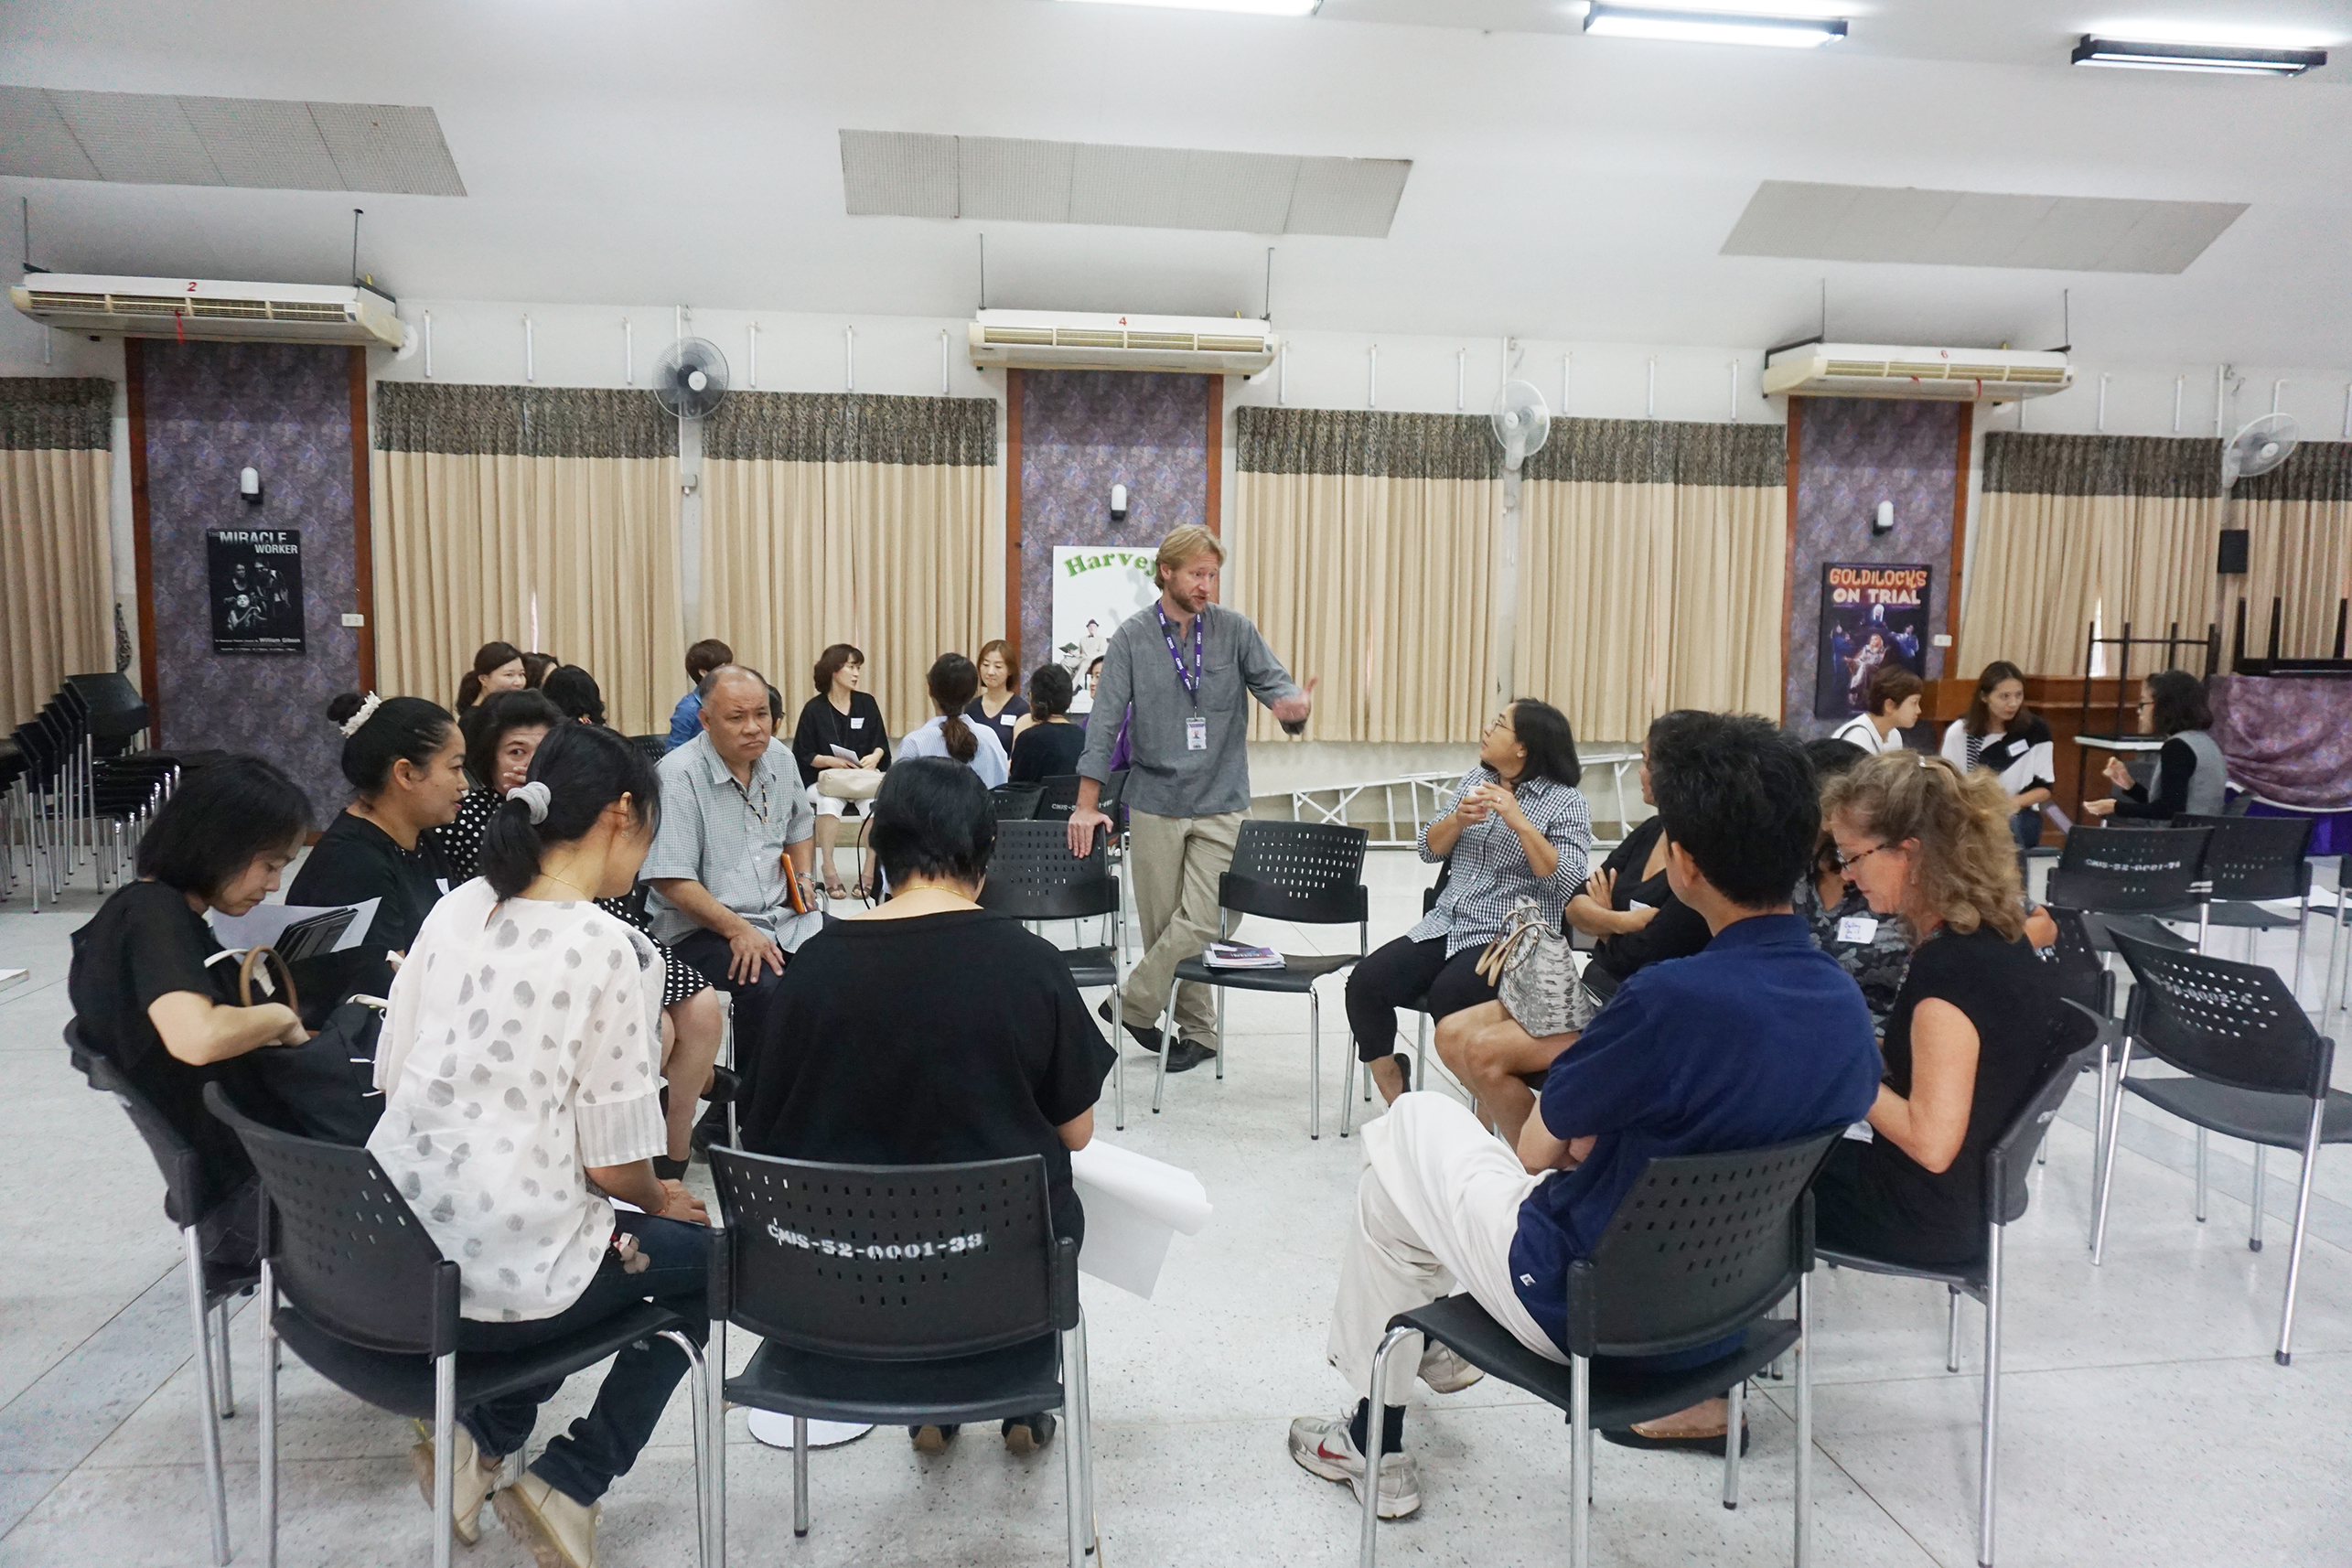
\includegraphics[width=\textwidth]{chapter4_a3.JPG}}


\minor{Additional Structures for Collaboration}

In addition, monthly Team Meeting Time and \href{https://docs.google.com/document/d/1tSEBD59kwf83Z0-m1Q4hzNrVwaJMHdracrghwqoSdW0/edit?ts=589d238c}{Early Release Professional Developments Days} are held for all teachers to collaborate, review student work, and plan instructional practices to improve student achievement. In addition, the faculty regularly reviews the definition of global citizenship during their professional development meetings and brainstorm ways for our students to practice being responsible, proactive members of the global community (e.g. \href{https://docs.google.com/a/cmis.ac.th/document/d/1fJmuufIbXlGt7DGAuQ3OBW00VdOY_1QgqLzgEpmxdKQ/edit?usp=sharing}{Cultural Heritage Flag Communication Group Activity}).

\href{https://docs.google.com/document/d/1eDtOzhe_JnpVQmEIoF-IO0ejVrDalm8s0i6PaiDl9hs/edit}{Instructional Rounds process}: see Curriculum, Instruction, and Assessment Chapter for more information. 

The K-12 Student Success Team has implemented Response to Intervention (RTI) model as a way of supporting all students and teachers through the use of positive (academic and behavioral) interventions. See the \href{https://docs.google.com/document/d/16bGCvdQuhHquFdigvip3H5YgfubNVMStl7UpOfCRcFk/edit}{Behavior Management Plan} for evidence. 

The \href{https://docs.google.com/a/cmis.ac.th/document/d/1iW_tWIwRlWU2p0oIOvd3usDsxj9qYDt_2ROwNPBTHSc/edit?usp=sharing}{Teacher Leadership Team} was established during the 2015-16 school year. This team of ten teachers was created to increase staff leadership roles and promote a shared responsibility and accountability to support student learning in a global environment. The team meets 3-4 times a semester with the administrative team to collaborate on ways to support PK-12 teachers with: instructional best practices, curriculum planning, assessment design, and data analysis. Meetings also review specific leadership skills such as facilitating meetings, creating a plan of action, and monitoring team progress.

In all divisions, the \href{https://docs.google.com/document/d/15_5X5QtixmWVheEUBVO9N1aislsLDm_ZW4-4g4YQ7F4/edit?ts=589d25d9}{teacher evaluation process}, regular classroom walkthroughs and informal and formal observations have all been modified and increased to further ensure collaboration and accountability for enhanced student learning.

\minor{So what}

Though the CMIS Leadership has developed multiple  initiatives for staff to increase shared responsibility, accountability, and collaboration opportunities.  In the future, CMIS will be including a more frequent focus on looking at student evidence to help in evaluating the effectiveness of these current initiatives. 
\end{findings}

\subsubsection{Evaluation of Existing Processes}

\indicator{The school leadership regularly reviews the existing processes to determine the degree to which actions of the leadership and staff focus on successful student learning and global citizenship.}

\prompt{To what extent does the school leadership regularly review the existing processes to determine the degree to which actions of the leadership and staff focus on successful student learning? Evaluate the effectiveness of the school leadership and staff to work collectively as a learning community in order to promote the desired global competencies.}

\begin{findings}
CMIS leadership regularly review existing processes to determine the degree to which actions of the leadership and staff focus on successful student learning and global citizenship.

In 2014 all teachers were trained and have since participated in the year long \href{https://drive.google.com/a/cmis.ac.th/file/d/0B71_pYxcTLo-OExlV0Y5UVFBNVU/view?usp=sharing}{Datawise Process}. Datawise is a school improvement process that organizes and brings coherence to the work of improvement. It is a specific process that facilitates intentional thinking and utilizing a more disciplined way of looking at student data as a collaborative group. Datawise helps all educators in all positions to learn how to analyze data in a manner that contributes to improved instruction and increased student learning. \href{https://docs.google.com/document/d/1TmnCp5qZiZAUMnUmaU32PBn2UGvCMVtFO8r5OsxwNo4/edit}{CMIS 2016-17 Datawise Plan}

Since 2014 all staff  have incorporated the \href{https://docs.google.com/a/cmis.ac.th/document/d/1IFIRIT2wAu1GF2yZ5FSSOdFB3yBKxzx_eCZhdFtroC0/edit?usp=sharing}{Datawise} agenda template when collaborating with colleagues. This template includes reviewing the norms of engagement, that the objective is aligned to increasing student learning, and that there is an assessment of how useful the meeting was in accomplishing the goal.

During the 2015-16 school year CMIS organized Teacher Table Talk sessions during early release days for staff to capture insights and suggestions about successful ways to increase student learning and promote global citizenship.

\minor{\href{https://drive.google.com/drive/folders/0ByVFfrm0zfolLTd2WjVNX0pWZU0?usp=sharing}{Instructional Rounds}}

Instructional Rounds were implemented at CMIS in 2015. They are structured observations between teachers and during the instructional round period, a great deal of data is collected which focus on teacher deliberative practice and student achievement. See sections entitled: Congruence and Collaborative Work for more information on instructional rounds. 

\minor{So what...}

A great deal of evaluation of the processes to determine student achievement have taken place over the past three years. For example, the initial review of the teacher evaluation instrument and process was found not to be aligned with current research or student achievement. CMIS Leadership and volunteer staff collaborated in piloting a more inclusive model prior to training all new staff the following year. This allowed CMIS to modify and adjust the process and ensure that student learning was the focus. 

The \href{https://drive.google.com/a/cmis.ac.th/file/d/0B71_pYxcTLo-OExlV0Y5UVFBNVU/view?usp=sharing}{Datawise process} has enabled CMIS Leadership and Staff to identify authentic areas for instructional improvement. For example, during the 2015-2016 school year, lack of consistent assessments among divisions was identified as a need and has been the focus for this year’s \href{https://docs.google.com/a/cmis.ac.th/document/d/1ioGkUkxTr5hRC_Vn4TDy7FcKHwcaWzBYNEeIConfXA4/edit?usp=sharing}{Datawise Department Action Plan}. CMIS should continue to implement the Datawise process with fidelity in order to meaningfully identify further areas for future improvement in student achievement.
\end{findings}

\subsubsection{Interconnectedness of the School to the World}

\indicator{The school leadership involves staff in assessing the school’s interconnectedness to the world to promote a globally minded culture.}

\prompt{Evaluate these processes and the results in relation to the school’s interconnectedness to the world to promote a globally minded culture.}

\begin{findings}
CMIS Leadership, teaching staff, and community organize and implement an \href{https://docs.google.com/a/cmis.ac.th/document/d/1YGCBI_uQVVcvOvw4c_Q2GcoJQzadFou1_6WtBAMTTaE/edit?usp=sharing}{International Day} that rotates with Thai Day (i.e. every other year); other major events such as Model United Nations and \href{https://docs.google.com/a/cmis.ac.th/presentation/d/1U8ieEOjf4gWWTdg-IU8Twcm2qywiETSM0itGHsq7oTg/edit?usp=sharing}{National History Day} are also scheduled. Each of these events showcase and celebrate CMIS’s unique place on the globe and their diverse global community. 

For the last two years CMIS focused on re-evaluating our definition of global mindedness and thinking of additional ways students can connect to their peers and support their local community.

This resulted in CMIS grade level field trips and school-wide activities focusing more closely to our mission of giving back both globally and locally. For example, middle school students travel to the Hope House orphanage where they plan and present team building activities. The CMIS annual Harvest Festival at elementary level includes activities to support a the same orphanage in an effort to strengthen the bond and support already established. The school-wide kindness challenge was an internationally recognized project and included a fundraiser for Hope House.

Weekly college visits from around the world during our secondary lunch times provide different perspectives and an interconnectedness for our students to the world an a globally minded culture.

\minor{So what...}

CMIS Leadership adheres to the research that states: ``...[global] dispositions are developed through enculturation'' (Ritchart, Church, \& Morrison, 2011). 

CMIS believes that students cultivate dispositions not though occasional units, or annual school events, but through ongoing participation in classroom cultures where these dispositions are visibly valued and practiced. CMIS will continue to find more opportunities for teachers to embed global dispositions routinely and naturally in their curricular and unit planning. 

Furthermore, data indicates that most student’s awareness of global issues and dispositions come only from their view that they study in an international school. It is widely understood that just being in an international school does not automatically ask student to address global issue or use global dispositions.
\end{findings}

\minor{Conclusions}

The findings suggest that CMIS addresses this criterion to a high degree. In an effort to increase student achievement further in this area CMIS plans to:

\minor{Maintain and Monitor:}
\begin{itemize}
\item Structures for strategic planning, regular communication, and meaningful conflict resolution. 
\item Communication and practice theses structure with the community
\end{itemize}


\minor{Investigate Better Practice:}
\begin{itemize}
\item Additional (research based) ways for students to apply and refine their global skills by practicing cultural awareness, creativity, collaboration, communication, problem solving, and empathy.
\end{itemize}


\subsection{A4 Staff Criterion}

The school leadership and staff are qualified for their assigned responsibilities, are committed to the school’s purpose and engage in ongoing professional development that promotes student learning in a global society.

\subsubsection{Employment Policies/Practices and Qualifications of Staff}

\indicator{The school has clear employment policies/practices related to qualification requirements of staff.The school reviews all information regarding staff background, training, and preparation, including international expertise.}

\prompt{Evaluate the clarity of the employment policies and practices related to qualification/statutory requirements of current and potential staff for all programs, including all types of online instruction and specialized programs such as college/career preparation.}

\begin{findings}
CMIS has always recognizes the need to hire suitably qualified people to fill its administrative, teaching, and non-teaching positions. After extensive research from the educational organizations CMIS has membership to:

\begin{itemize}
\item The International School Association of Thailand (\href{http://gallery.cmis.ac.th/2016-2017/ISAT-Regional-Meeting/}{ISAT})
\item The East Asia Regional Council of Schools (\href{https://www.earcos.org/}{EARCOS})
\item Association of Christian Schools International (\href{https://www.acsi.org/}{ACSI})
\item The Association for Supervision and Curriculum Development (\href{http://www.ascd.org/about-ascd.aspx}{ASCD})
\item Academy for International School Heads (\href{http://aishbank.squarespace.com/}{AISH})
\item National Association of Independent School (\href{http://www.nais.org/Pages/default.aspx}{NAIS}) 
\end{itemize}

The School management team realized that some of their policies were outdated and did not reflect current research, especially in terms of global competency. Beginning 2016-17 school year they developed more defined employment policies and practices of potential staff:

Current Requirements:
\begin{itemize}
\item Current certification in home country
\item Original documentation verifying credentials
\item 3 confidential reference checks
\item First interview with immediate supervisor/team
\item Second interview with Superintendent and Principal
\item Third interview with SET
\item Clearance of criminal background check
\item Signed agreement to child abuse policy
\item Signed agreement to contractual obligations
\item Completion of new staff orientation
\item Completion of probationary period
\end{itemize}

These requirements are outlined in the \href{http://cmis.ac.th/about/employment}{employment section} of the CMIS website and on the our recruitment sites (e.g., The International Educator). CMIS believes that student learning benefits greatly from a highly qualified and trained team, and school leadership is committed to continuing to recruit highly qualified and effective staff to advance the school’s purpose and core values.

The updated expectations have required some of our existing staff to renew their certification and clearance documentation. ALL staff are currently in the process of doing so with the support and guidance of the Human Resources department.

\minor{So what...}

CMIS has worked hard to improve and strengthen their employment strategies. Their efforts have solidified the need to remain up to date with global employment practices that focus on recruiting practices that obtain and retain the most capable staff.
\end{findings}

{\centering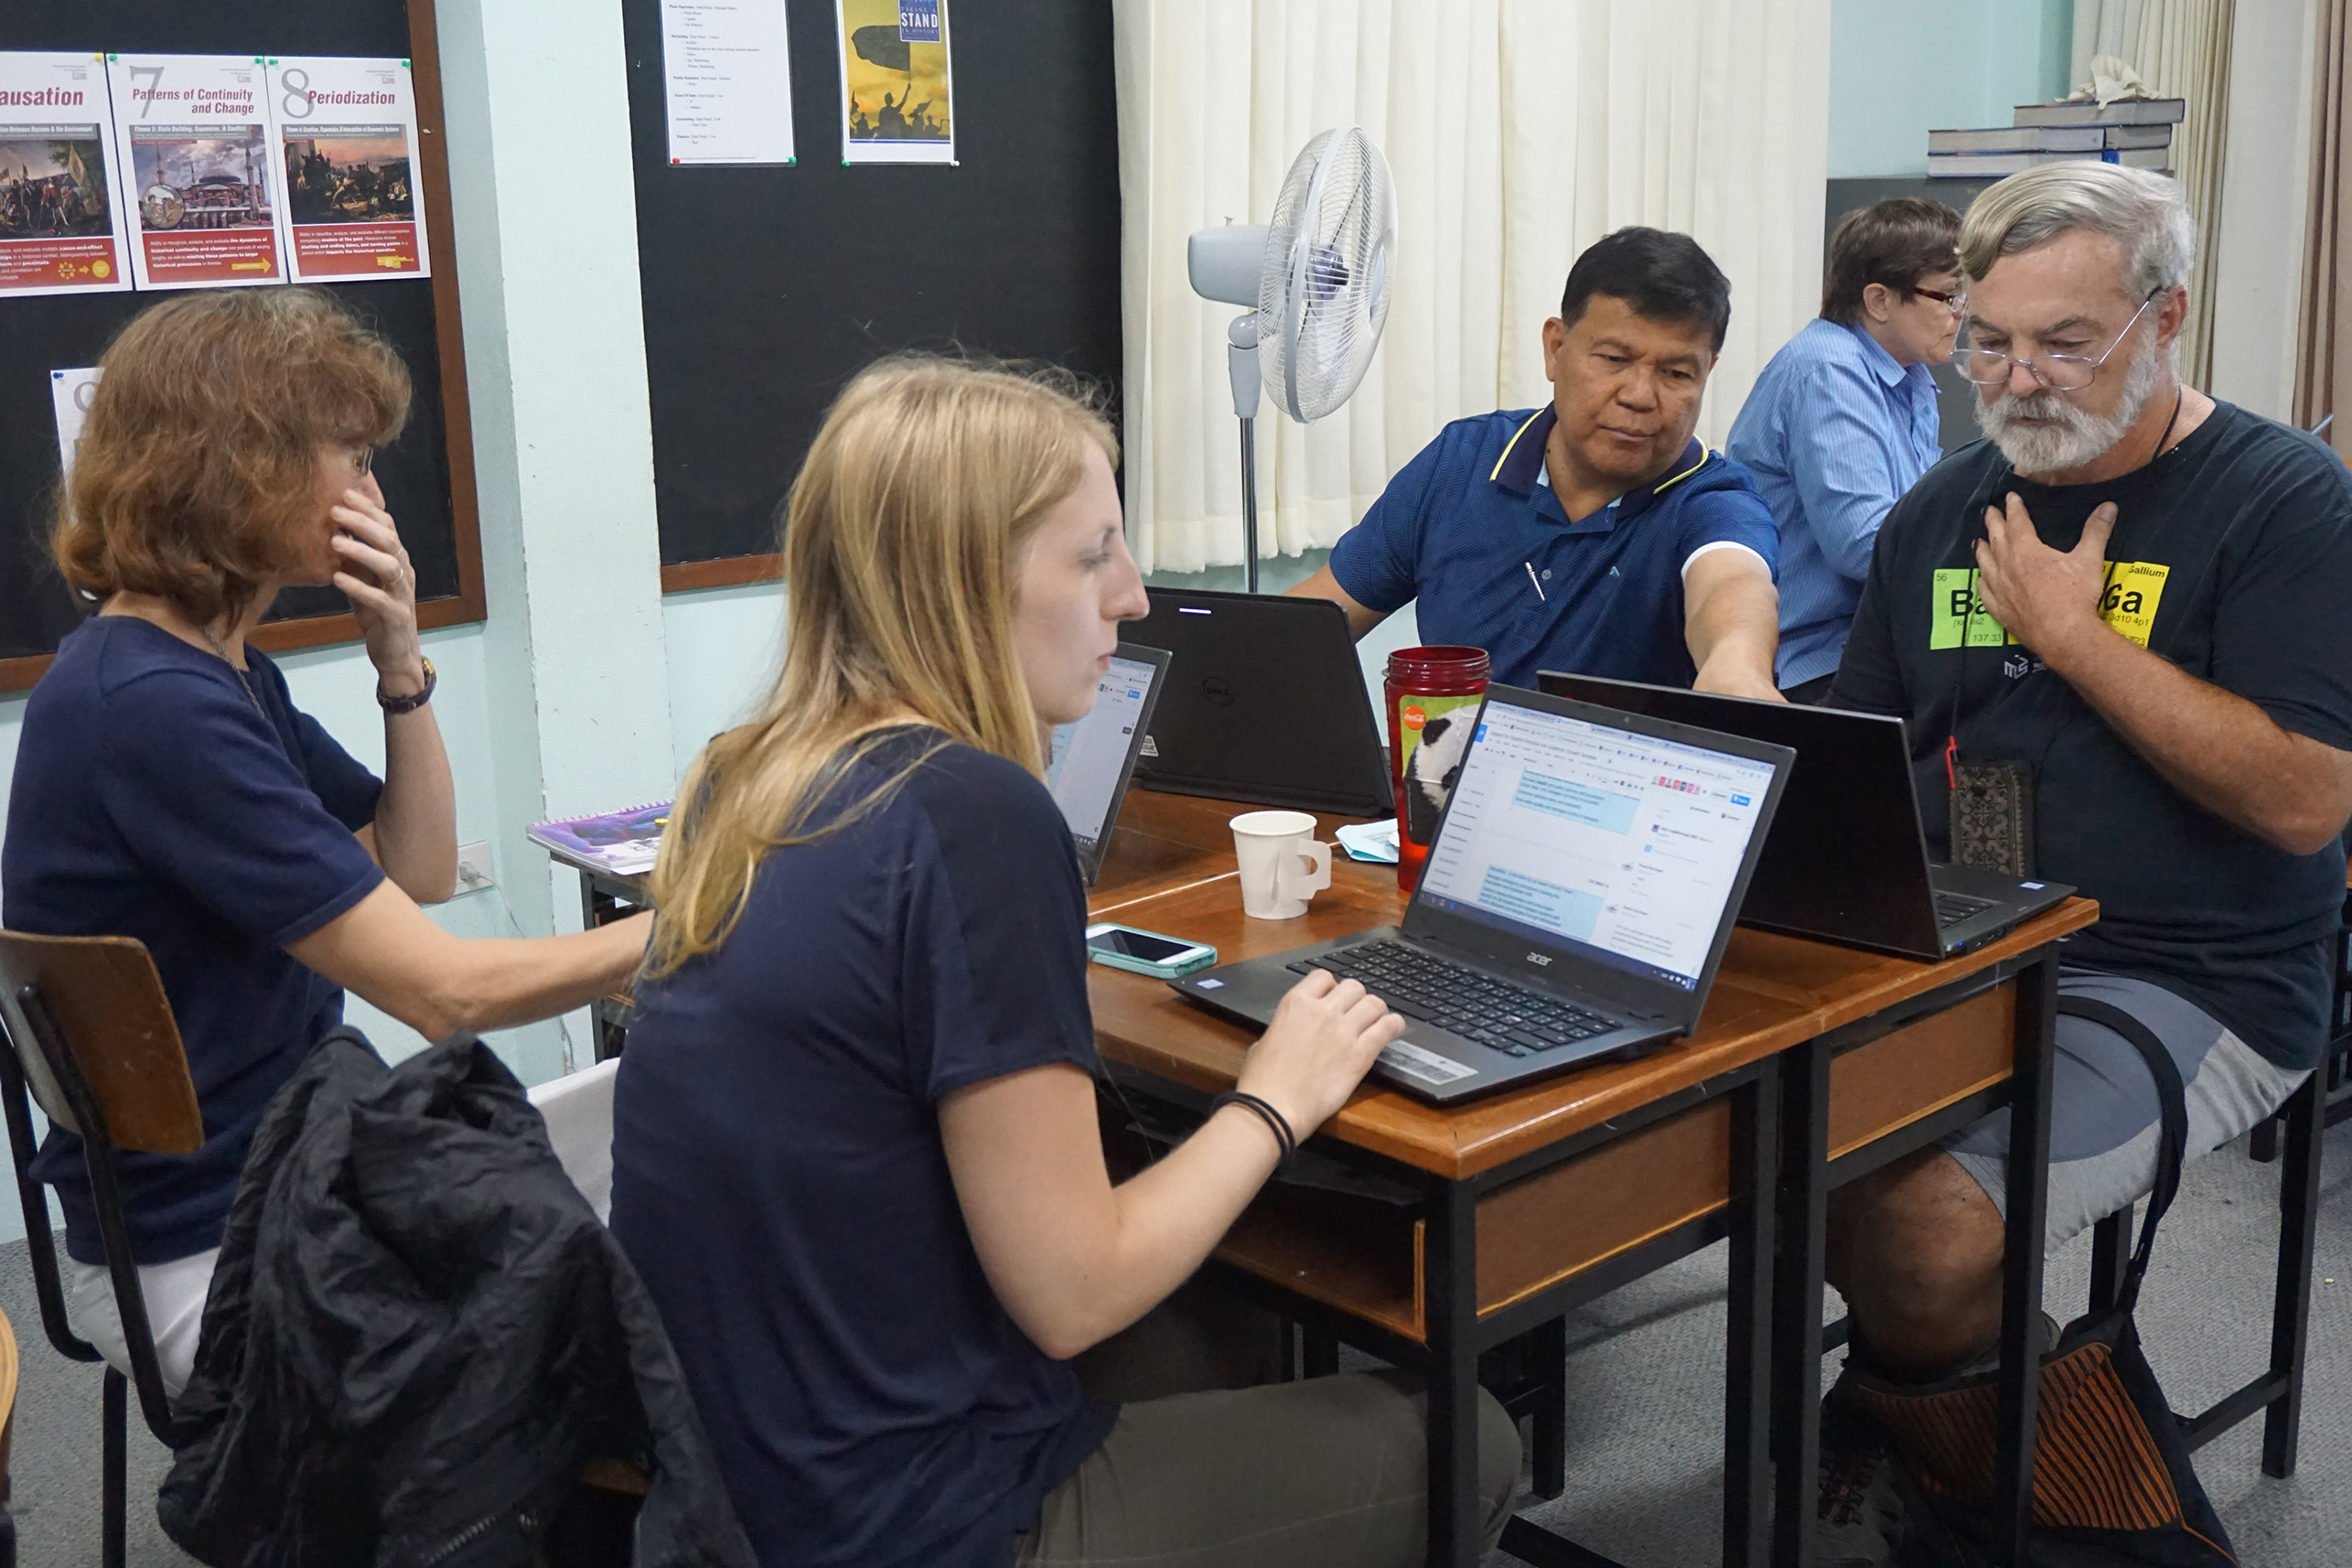
\includegraphics[width=\textwidth]{chapter4_a4.JPG}}
 
\subsubsection{Maximum Use of Staff Expertise}

\indicator{The school has a process to assign staff members and provide appropriate orientation for all assignments, including online instruction and specialized programs so that the expertise of the staff members is maximized in relation to impact on quality student learning.}

\prompt{Evaluate the process to assign staff members and provide an appropriate orientation process to ensure all staff are qualified and prepared or their responsibilities including any type of online instruction}

\begin{findings}
In 2015-2016 school year an Human Resources and Registrar position was created to assist staff with additional support  and guidance.During the 2016-17 school year an additional Human Resources assistant position was enlisted to create an Human Resources department. As well as help with salaries and benefits, this department also assists staff and parents with visa, permit, and governmental requirements.

Last year, CMIS established a New Staff Welcoming Committee. The main objective of this committee  was to create a smooth transition for all new staff and help them prepare all necessary paperwork and documentation. In addition, new staff members were provided with 5 days accommodation at on-site housing in an effort to improve the transitional period especially as the majority of our new hires are travelling from different countries.

This year, CMIS created a New Hire Buddy Program where current staff volunteer to “adopt” a new hire in an effort to make the personal transition to Chiang Mai as seamless as possible. New staff  are also assigned a Team Leader to assist them with curriculum and instructional support. Starting last year, new hires begin the school year a week earlier than returning staff to participate in New Staff Orientation programs and a Thai Culture training curriculum.

Based on feedback from new staff, the 2016-17 New Teacher Orientation was extended to include more time to work in classrooms, plan with colleagues, and manage personal needs (e.g. accommodation and travel)

Based on feedback from new staff, the Returning Staff Orientation has been modified to include  more opportunities for returning staff to collaborate with new faculty, receive training updates (e.g. Data wise, Ubd, Powerschool etc.) and work within their departments.

\minor{So what...}

CMIS worked hard to increase the opportunities for appropriate orientation to all staff. We understand that this additional support increases the expertise of the staff members is maximized in relation to impact on quality student learning. CMIS leadership believes that they can increase these opportunities further and are currently working with staff to explore additional ways.
\end{findings}Findings

\subsubsection{Defining and Understanding Practices/Relationships}

\indicator{The school has clear administrator and faculty written policies, charts, and handbooks that define responsibilities, operational practices, decision-making processes, and relationships of leadership and staff.}

\prompt{Evaluate the administrator and faculty written policies, charts, pacing guides and handbooks that define responsibilities, operational practices, decision-making processes, and relationships of leadership and staff. Determine the degree of clarity and understanding of these by administration and faculty.}

\begin{findings}
CMIS has clear written policies and \href{https://drive.google.com/a/cmis.ac.th/file/d/0Bwny3HLdIIS7RF9veFk5UXB2Q2M/view?usp=sharing}{organizational charts} that define responsibilities, operational practices, decision-making processes, and relationships of leadership and staff. These policies and procedures are reviewed and updated at the beginning of the year with all staff during the staff orientation.

Additional procedures and expectations can be found in the \href{https://docs.google.com/a/cmis.ac.th/document/d/1DrXVXsgw4U62HCGOceOKsgC8V1LDQFhHKgDB35oq4wY/edit?usp=sharing}{Faculty Handbook} which is updated and made available to staff as a Google document on a yearly basis. Policy and procedural updates are communicated during staff orientations, department, team leader and divisional meetings.

\minor{So what...}

CMIS understands the importance of having clearly written policies, and handbooks that define responsibilities, operational practices, decision-making processes, and relationships of leadership and staff. 

The CMIS faculty handbook has grown considerably in volume over the last few years and recent staff feedback has indicated that it can be difficult to navigate. In an attempt to address this concern the administration and team leaders have been working together to create a more streamlined and useful  2017-18 edition. 

Staff feedback (from TACT) this year indicated that the \href{https://docs.google.com/a/cmis.ac.th/presentation/d/18ekiAcUSiwa7oJM9tdwe2OSfnC_47RkbLz8ZjEt6O9I/edit?usp=sharing}{policies update presentation} this year was overwhelming for some staff and when presented as a whole group it was not conducive to open discussion. The leadership appreciated this feedback and apologized in person to the staff and resolved to present next year's presentation in small groups and in segments. 
\end{findings}

\subsubsection{Staff Actions/Accountability to Support Learning}

\indicator{The school evaluates the effectiveness of the processes and procedures for involving staff in shared responsibility, actions, and accountability to support student learning throughout all programs. This includes an evaluation of the collegial strategies used to implement innovations and encourage improvement, such as shadowing, coaching, observation, mentoring, and group presentations.}

\prompt{How effective are the processes and procedures for involving staff in shared responsibility, actions, and accountability to support student learning throughout all programs? Provide representative examples and data regarding impact on student learning.}

\begin{findings}
CMIS Leadership has provided processes and procedures to address shared responsibility and accountability. 

\minor{Collaborative Structures}

CMIS Leadership provides time for professional development and collegial discussions through the scheduling of meetings throughout the calendar year. Teachers meet as whole staff, department, divisional, and a Teacher Leadership Team to discuss different topics (e.g. integration, looking at student work, unit planning, cohesion, best practices etc). Whole staff meetings are normally reserved for specific professional development training. 49 out of 59 responses to the last professional development survey responded that the topics presented: 

\begin{itemize}
\item positively challenged the way [they] approach instruction, assessment, and planning; 
\item strengthened [their] understanding and application of instruction, assessment, and planning or; 
\item provided [them] with a solid foundation in which to grow my understanding of the topics.
\end{itemize}

See \href{https://docs.google.com/a/cmis.ac.th/forms/d/1-00JLey-jyLuizymm8z8JGJ6iLp4l-ccsTgHJ_Ckcj8/viewanalytics}{Professional Development Reflection} for more information. 

During the 2014-2015 school year, a great deal of professional development time was used to discuss and unpack the new literacy standards. One of the most critical design considerations of the standards is that they are a shared responsibility of all staff members. Each teachers, regardless of what they teach, have literacy standards. This discussion manifested into practice by adding key literary elements to the UbD unit template that all teachers must complete. See \href{http://www.corestandards.org/ELA-Literacy/introduction/key-design-consideration/}{Key Design Considerations} for more information. 
		
\href{https://docs.google.com/a/cmis.ac.th/presentation/d/1j9DjUPHbIprWWbftcBxiF35BKmzU5C_lW9Z78f8CAeE/edit?usp=sharing}{\minor{Instructional Rounds}}
The peer observation process provides another opportunity to involve staff in actions to address and support student learning. Instructional Rounds asks teachers to collect observational data on their colleagues, based upon a focus question that the teacher being observed chooses. By keeping the process free from evaluation and judgements, many teachers were able to view their practice objectively. The feedback was very positive. Some of the comments from participants include:

``It was a positive experience seeing my colleagues teach for the first time in five years”
``Having feedback from co-teachers is always helpful''
``Thanks for creating an environment/atmosphere that is non-threatening''
``Great to see other classes, get ideas from colleagues on student engagement''
``Inspired more and deeper conversations on what’s ‘measurable’''
``It genuinely answered a question that I could not effectively answer myself'' 

\minor{So what...}

Though CMIS uses processes and procedures to engage staff in shared responsibility, actions, and accountability, more time should be devoted to obtaining examples and data regarding impact on student learning.
\end{findings}

\subsubsection{Support of Professional Development}

\indicator{The school effectively supports professional development/learning with time, personnel, material, and fiscal resources to facilitate all students achieving the academic standards and the schoolwide learner outcomes. Teachers are involved in experiences such as visits, exchanges, and professional development to strengthen their understanding of global competencies.}

\prompt{How effective is the support of professional development/learning with time, personnel, material, and fiscal resources to facilitate all students achieving the academic standards and the schoolwide learner outcomes? Provide evidence and examples.}

\begin{findings}
The CMIS Leadership Team supports teacher professional development in a variety ways and is guided by current research. 

See the sections in the Curriculum, Instruction, and Assessment category entitled, Professional Collaboration and the Professional Development for details on how CMIS promotes and implements professional development opportunities. Subsections of the Professional Development indicator includes:

\begin{itemize}
\item Backed by Research
\item Early Release Wednesday
\item Consistency 
\item Outside Presenters
\item Chiang Mai Circle of International School (CMCIS) 
\item Other Professional Development Opportunities
\item Outside Professional Development 
\item CMIS Professional Development Fund 
\end{itemize}

\minor{So what...}

As noted in the Curriculum, Instruction, and Assessment category, professional development at CMIS is a priority. Though CMIS Leadership and Staff will continue to focus on reflective, genuine, deliberate teacher training, how the leadership and staff transition this information to the classroom and what accountability measures should be in place will continue to be a goal in the near future.
\end{findings}

\subsubsection{MISSING SUBSUBSECTION TITLE}

\indicator{The school supports professional learning of the staff members that develops their use of important skills that are inherent in developing the global competencies of the students; these include collaboration, communication, creativity, and problem-solving.}

\prompt{Evaluate the effectiveness of the professional learning in relation to global competency skills being applied in individual classes and the learning results.}

\begin{findings}
CMIS Leadership supports professional development for staff that helps them support student collaboration, communication, creativity, and problem solving.

Teacher professional development at CMIS uses discussion protocol and structures to promote staff collaboration, communication, creativity, and problem solving. The facilitators review and encourage the teaching staff to use those protocols in their classrooms to promote the practice of these global competency skills. The following is just a sample of the different protocols that have been shared:

\begin{itemize}
\item save the last word,
\item appointment clock 
\item notices and wonderings
\item warm and cool feedback
\item passion profiles
\item hopes and fears
\item STR (Stop, Think, and React)
\item circle of voices
\item world cafe
\end{itemize}

The CMIS leadership have also provided professional development workshops to develop students problem solving skills. These workshops included What is Productive Failure? (2014), Language and Learning in Math (2015), and Focus, Coherence, and Rigor in Mathematics (2016)

\minor{So What...}

CMIS has been fortunate enough to have some teachers attend quality professional development.  CMIS will continue to monitor and maintain professional development requests to ensure that they are addressing not only the standards, but indicators of global learning.
\end{findings}

\subsubsection{Supervision and Evaluation}

\indicator{The school implements effective supervision and evaluation procedures in order to promote professional growth of staff in 21st century skills and thinking. Teachers regularly reflect on their approaches to develop global competencies in the students.}

\prompt{How effective are the school’s supervision and evaluation procedures?}

\begin{findings}
CMIS utilizes effective supervision and evaluation procedures in order to promote professional growth of staff in 21st century skills and thinking. Teachers regularly reflect on their approaches to develop global competencies in the students.

During the 2014-2015 school year the \href{https://docs.google.com/document/d/15_5X5QtixmWVheEUBVO9N1aislsLDm_ZW4-4g4YQ7F4/edit?usp=sharing}{CMIS Teacher Observation Tool} was modified and updated to include the findings of the research based report, \href{https://drive.google.com/a/cmis.ac.th/file/d/0Bwny3HLdIIS7bXJ0dEpCWG51MTQ/view?usp=sharing}{Essential Practices of High Quality Teaching and Learning}. The study analyzed recent educational literature an existing rubrics and frameworks that focus on the practice of effective teaching, and constructed a list of core, essential practices of high quality teaching and learning that cuts across all content areas and grade levels. 

The CMIS teacher evaluation process was also updated to include a more comprehensive self reflection and self-assessment component. These 21st century, critical thinking skills were added to reflect the CMIS understanding that, ``Research has clearly demonstrated that the effects of reflection improve teaching. Using a framework to guide such reflection enhances the value of the activity and makes teaching more purposeful, thoughtful, and rewarding.'' -\href{http://www.ascd.org/publications/books/106034/chapters/Using-the-Framework.aspx}{Charlotte Danielson} 

The updated CMIS teacher evaluation model focuses on the teacher reviewing observational data to identify student learning, increase student learning opportunities and promote desired student global competencies. The  model encourages CMIS teachers to reflect deeply on their practice through a common framework and vocabulary. It helps teachers determine the focus of their professional development based on what is actually occurring (or not occurring) in their classroom, and set meaningful goals for increased student achievement. (example).

Teacher feedback has indicated that they find the CMIS evaluation process to be meaningful and supportive,  

\blockquote{``This is the first school in my experience as an educator that makes the observation process feel natural, non-threatening, and meaningful. Rather than my whole year being "judged and critiqued" based on one class, I felt supported and encouraged. At previous schools, the observation process felt intimidating and was often just something checked off of a list. At CMIS, being involved in the process from the beginning to the end and having genuine conversations about future classroom goals felt like true growth.''}
                                                                                            -CMIS Middle School Teacher

\minor{So what...}

CMIS has a highly effective school supervision and evaluation process. The updated procedures promote professional growth of staff in 21st century skills and thinking. Teachers are asked to regularly reflect on their practices and develop global competencies in their students (i.e. student learner outcomes). 
\end{findings}

\subsubsection{Measurable Effect of Professional Development}

\indicator{There are effective operating processes that determine the measurable effect of professional development, coaching, and mentoring on student performance.}

\prompt{Comment on the effectiveness of the processes in determining the measurable effect of professional development, coaching, and mentoring on student performance. Provide evidence about whether the professional development/learning has had a positive impact on student learning, e.g., developing the students’ global competencies.}

\begin{findings}
For school wide opportunities, all professional development planning has been aligned to best practices and the existing adult learning research. 

\minor{Professional Development Efficacy}

CMIS Leadership adheres to current research which states that teachers who receive well-designed professional development, for an average of 45 hours (CMIS literacy/assessment focus was at approximately 40 hours in 2014-2015) spread over six to 12 months, can increase student achievement by as much as 21 percentile points (Yoon, Duncan, Lee, Scarloss, and Shapley, 2007). CMIS Leadership would like to encourage moving away from the one-shot, "drive-by," or fragmented, "spray-and-pray" workshops lasting 14 hours or less which show no statistically significant effect on student learning (Darling-Hammond, Wei, Andree, Richardson, \& Orphanos, 2009). Above all, CMIS Leadership would like to continue to move towards implementing effective professional development programs are job-embedded and provide teachers with five critical elements (Darling-Hammond et al., 2009)  which include: collaborative and active learning, linking professional development topics with content specific teaching, and deeper content knowledge (see section entitled Professional Development in the Curriculum, Instruction, and Assessment category).

\minor{Literacy/Assessment Professional Development of 2014-2015}

As mentioned, the only professional development the CMIS Staff has engaged in that was close to the 40 hour threshold was the Literacy/Assessment trainings of 2014-2015. Data from that time indicates that a majority of the participants have confidence in their ability to address the topics discussed, such as implementing the literacy standards (57\% stated confident or very confident), balancing literature with informational text (60\%), literacy standards in history and science (47\%), text complexity (34\%), academic vocabulary (72\%), and close reading (55\%). The Literacy/Assessment training of 2014-2015 was successful in improving the teachers confidence in using these shifts in instruction for most of the topics. 

\minor{Understanding by Design}

CMIS Teaching Staff are required to develop Understanding by Design plans for their content units. The CMIS UbD unit goes further than the traditional UbD template by adding a handful of modifications to ensure congruence between our skills/knowledge, our adopted standards, and the SLOs within the unit; see \href{https://docs.google.com/a/cmis.ac.th/document/d/1wwb5O3EmHNmzx7MOdHvi0TFjyYRWyELnyD1VRsmuj1Y/edit?usp=sharing}{Table 1}.  This has been adopted to ensure that the topics addressed during the professional development trainings (e.g. text complexity, close reading, formative assessment, DOK) are being applied during planning. 

\minor{So what...}

At CMIS professional development is a priority. CMIS Leadership should continue to develop and plan professional development opportunities that require over 45 hours of commitment to ensure a positive effect on student achievement. This 45 hours does not have to be seat time and can be planned as instructional rounds, PLCs, or datawise;  as long as the staff is focusing on one concept. Additionally, though elements have been added to the UbD units to address our professional development topics, time and resources need to be spent  to measure their effectiveness. 
\end{findings}

\subsubsection{Conclusions}

The findings suggest that CMIS addresses this criterion to a high degree. In an effort to increase student achievement further in this area CMIS plans to:

\minor{Maintain and Monitor}

\begin{itemize}
\item Employment strategies that remain up to date with global practices that focus on recruiting to obtain and retain the most capable staff.
\item Opportunities for appropriate orientation to all staff. 
\item Comprehensive, research based professional development opportunities for ALL staff
\end{itemize}

\minor{Investigate Better Practice}
\begin{itemize}
\item Additional (research based) ways for CMIS to continually hire qualified staff who are committed to the school’s purpose and engage in ongoing professional development that promotes student learning in a global society.
\end{itemize}




\subsection{A5 School Environment Criterion}

The school has a safe, healthy, nurturing environment that reflects the school’s purpose and is characterized by respect for differences, trust, caring, professionalism, support, and high expectations for each student.

\subsubsection{Caring, Concern, High Expectations}

\indicator{The school demonstrates caring, concern, and high expectations for students in an environment that honors individual and cultural differences.}

\prompt{To what extent does the school demonstrate caring, concern, and high expectations for students in an environment that honors individual differences and is conducive to learning?}

\begin{findings}
CMIS demonstrates caring, concern, and high expectations for all community members in an environment that honors individual and cultural differences.

The Virtues Project was established at the elementary level in 2013 and is a globally recognized initiative used to inspire kindness, justice, and integrity in schools worldwide. It highlights ways for educators to use character virtues as a foundation to create safe, caring, and high performing learning communities. 

During 2015 the virtues were highlighted at the MS level during Health and Wellness classes, where they reviewed virtues and initiated \href{https://docs.google.com/forms/d/e/1FAIpQLScP9Fpphz10qaY0S4RO3VLKBQ54RC3WQdP-FGIBbPOcXzMwpQ/viewform?c=0&w=1}{random acts of kindness campaign}. At the beginning of the 2016-17 school year the virtues were acknowledged and practiced school-wide.

\minor{Examples}

In September 2016, middle and high school students focused on the monthly virtues of respect  and trust  which are essential  components for creating a caring and respectful environment that honors individual differences.

In February 2017, the school counselors facilitated a school-wide \href{https://docs.google.com/a/cmis.ac.th/document/d/1PsHRple71FshloSGrqvYHgQQCYx9_CwCsbtlMAkb-Aw/edit?usp=sharing}{Great Kindness Challenge} (GKC) to highlight the monthly virtue of kindness.\href{https://dochub.com/roneldanelcapadona/gDPKV2/gkc?dt=ysuio255qfhtbryf}{ The Great Kindness Challenge} is a globally recognized, proactive and positive bullying prevention initiative that has been shown to improve school climate and increase student engagement. CMIS also used it as a fundraising opportunity to raise money for a local orphanage and as a meaningful way to promote the CMIS Virtues Project school-wide

\href{https://docs.google.com/a/cmis.ac.th/document/d/1Mv1xjTpbY36naur8SDt9GanKNfR7YtYVL-bWwGLPSHo/edit?usp=sharing}{Monthly Virtue Assemblies} at the elementary level are performed by each grade level and focus on the importance of each virtue and how they help CMIS to live harmoniously together. The Awesome Eagles Program was launched in the Fall of 2014 to foster teamwork and encourage CMIS elementary staff to recognize and reward students when they witness an act of kindness, cooperation, and empathy. The students work together to collect Eagle Bucks for their class. The grade level with the most Eagle  Bucks each month is announced at the Virtue Assembly after which they celebrate with a class trophy and an ice cream party.

Thai Day and \href{https://docs.google.com/a/cmis.ac.th/document/d/1YGCBI_uQVVcvOvw4c_Q2GcoJQzadFou1_6WtBAMTTaE/edit?usp=sharing}{International Day} are school-wide traditions that highlight the high expectations CMIS holds for all community members in terms of respecting global values and appreciating cultural differences. 

With the addition of a counselor position at the middle school level in 2014, CMIS now has a counselor available at each division: elementary, middle and high school. They are part of the CMIS Student Success Team and develop strategies with students, teachers, administrators, and parents to help students be academically, emotionally, and socially successful. Some of the ways they do this are by:

\begin{itemize}
\item Providing individual and small group counseling based on student needs
\item Working with students to develop effective organization, time management, and study habits
\item Helping students set realistic academic and career goals and develop a plan to achieve them
\item Teaching classes on topics such as bullying, parenting, health, and planning for college or careers after graduation.
\item Identifying and reporting possible cases of neglect or abuse
\item Referring students and parents to resources outside the school for additional support
\end{itemize}

With the addition of a Student Service Coordinator position in 2015, the \href{https://docs.google.com/a/cmis.ac.th/presentation/d/1sWhr1U3qZIGEu2aQdWOl0OQ5Rkd8iRGWmUlszEJLz2o/edit?usp=sharing}{CMIS Student Success team} was established. This team consists of the health officer, counselors, and the learning support teachers. They meet regularly to review student achievement,  safety and wellbeing. If teachers have concerns related to their students they are encouraged to reach out to the Student Success Team facilitated by the Student Service Coordinator. There is a \href{https://docs.google.com/a/cmis.ac.th/forms/d/e/1FAIpQLScVtFtaEXarGOjwsiJyGdbLAMbeNzG9m44i1fWXFLbtMKZcUg/viewform}{Student Service Request Form} available on the teacher dashboard section of the CMIS Handbook.This form activates immediate support from the team to meet with the teacher and create a plan of action.

\minor{So what...}

CMIS works hard to create a student centered environment that models genuine caring, concern, and high expectations for ALL. CMIS aims to always maintain an environment that honors individual differences and is conducive to learning. CMIS understands that a nurturing school climate is crucial for student learning and looks forward to finding additional ways to strengthen it.
\end{findings}

\subsubsection{Student Self-Esteem}

\indicator{The school fosters student self-esteem through high expectations for each student and recognition of successes.}

\prompt{To what extent does the school foster student self-esteem through high expectations for each student and recognition of successes?}

\begin{findings}
CMIS fosters student self-esteem through high expectations for ALL students and recognition of successes.
CMIS helps students to understand that self-esteem is how we value ourselves; it is how we perceive our value to the world and how valuable we think we are to others. The following are some outward student attributes of positive self-esteem that are described in our student learner outcomes and illustrated in our CMIS \href{http://cmis.ac.th/about/vision}{Vision Tree}. 

\begin{itemize}
\item Flexibility
\item Resilience
\item Courage
\item Self-direction 
\item An ability to make mistakes and learn from them 
\item An ability to accept mistakes from others 
\item An ability to solve problems 
\item An ability to trust others 
\end{itemize}

CMIS believes that publicly recognizing student’s thinking and accomplishments can benefit their learning and the overall school climate. It also believes that recognition needs to be authentic and meaningful.

Some examples are:
\begin{itemize}
\item Providing opportunities for students to voice their opinions (e.g. Stuco meetings with Superintendent, cafeteria student survey, communication group discussions etc.)
\item Weekly “shout outs” of students who have achieved outside of school on \href{http://blogs.cmis.ac.th/eagles/friday-september-16-2016/}{CMIS weekly announcements} (athletics, contests, performances etc)
\item\href{https://docs.google.com/a/cmis.ac.th/document/d/1DgY3NXB6m6qvmWnaRr2B2jswCGHRjaPFNPJA2Xzk1qw/edit?usp=sharing}{ Middle School Awards Assembly} for students that have demonstrated excellence in academics, athletics, the arts, and global citizenship
\item H\href{https://docs.google.com/document/d/1pxioSUeOgKZ4dT1jA9DiVzDjZjtrxuM-Gjqh7fRy0Us/edit?usp=sharing}{igh School Awards Evening} for students that have demonstrated excellence in leadership, academics, athletics, the arts, and global  citizenship.
\item ES and MS teachers recognize students of the month who have demonstrated resilience in their learning.
\item Student work is displayed on campus and on the website. 
\item Students encouraged to share their expertise by competing in local and international competitions (National History Day, MUN , poetry  etc.)
\end{itemize}

\minor{So what}

CMIS works hard to foster student self-esteem through high expectations for each student and recognition of successes. It understands the importance of having opportunities for students to reflect on how positive self-esteem gives them the strength and flexibility to take charge of their lives and grow from their mistakes without the fear of rejection. CMIS will continue to find new ways to encourage positive student self-esteem and recognize student achievement. 
\end{findings}

{\centering\includegraphics[width=\textwidth]{chapter4_A5.jpg}}

\subsubsection{Mutual Respect and Communication}

\indicator{Mutual respect and effective communication among and between staff, students, and parents is evident. There is understanding of the importance of cross-cultural communication in improving teaching, learning, and management.}

\prompt{What evidence supports mutual respect and effective cross-cultural communication among and between staff, students, and parents?}

\begin{findings}
CMIS believes that cultural awareness is the key to effective cross-cultural communications. 

CMIS defines cultural awareness as the ability to empathize that a person's behaviors and reactions can be culturally driven and that while they may not match our own, they are culturally appropriate. It believes that acceptance of all CMIS community members is essential and standards for respectable behavior need to be regularly revisited. 

\minor{Examples}

\begin{itemize}
\item During staff meetings the following Norms of Conduct are reviewed at every meeting:
\item Be present (mindful)
\item Respect time
\item Be adaptive
\item Be true
\item Assume positive intent
\item Ground statements in evidence
\end{itemize}

During CMIS staff and parent meetings the Pluses and Delta protocol is used to elicit feedback from the meeting participants about the meeting effectiveness. By using Plus/Delta, CMIS teams can continuously improve meetings and show respect for people by discussing the value of or ability to improve the time spent together. Providing an opportunity for constructive criticism demonstrates attentive listening, and mutual respect--skills that CMIS want to model positively to all  students.

When communicating with staff, students and parents the CMIS leadership tries to keep in mind that even though English is considered the international language of the school, the majority of the community who speak English are not native speakers.When communicating cross-culturally, CMIS makes particular efforts to keep communication clear, simple and unambiguous. It also ensures that translators are available at school events.

\minor{Examples}

There is a PTG meeting monthly that fosters communication between the parents and the school. Topics for discussion are \href{https://docs.google.com/a/cmis.ac.th/document/d/1kiwakkg8eKdtEexCxVNx-m1CfC3VqxhukDy8WXDPGKY/edit?usp=sharing}{parent generated}  and based on parent feedback. The school management and parent translators are always present for support.

Once a semester, there is a parent teacher conference where teachers, students, administrators, and parents come together and discuss the growth of their respective students. \href{https://docs.google.com/a/cmis.ac.th/document/d/1XA31w9WsFCzB3k9LcQnU46sTUmMeEiObDQ8yOqCPZdU/edit?usp=sharing}{CMIS National Honors Society} students are available as parent translators.

CMIS has a \href{https://docs.google.com/a/cmis.ac.th/document/d/1yZyHuHhAg7tHITOtlZQdX_w4kinRwL6J_Y_zco_7jSE/edit?usp=sharing}{Korean Liaison} fully devoted to communication across culture and language to Korean families.

\minor{So what...}

CMIS believes that mutual respect and effective communication among and between staff, students, and parents is crucial for a positive learning environment. It models cross-cultural communication to improve student achievement through teaching, learning, and management.
\end{findings}

\subsubsection{Teacher Support and Encouragement}

\indicator{There is a level of support and encouragement for teachers to use innovative approaches to enhance student learning.}

\prompt{How effective is the level of support and encouragement for teachers to use innovative approaches to enhance student learning?}

\begin{findings}
During CMIS professional development opportunities teachers learn different strategies to promote innovative teaching to enhance student learning.

\minor{Examples}

In 2015 CMIS hosted a region-wide workshop that focused on \href{https://docs.google.com/forms/d/e/1FAIpQLSdK2QvcDZyM_yfhT22BgModehhwhn3I8Ps6VoW2EIzaK-qing/viewform?c=0&w=1}{ Innovative Teaching and  ELL Learners} and invited educators from seven neighboring international schools to attend as well as all CMIS staff. 

In August 2016 all CMIS teacher received CMIS training on \href{https://docs.google.com/a/cmis.ac.th/presentation/d/1S1x1yEj7KDD6jM7u1RdTZJEt10_0r6mcJ-LmRb6iPWs/edit?usp=sharing}{Productive Failure}  based on the findings of Dr. Manu Kapur, Associate Professor of Curriculum, Teaching, and Head of Learning at Learning Sciences Lab in Singapore. CMIS teachers learned that productive failure affords better conceptual understanding, creative thinking, and helps students to transfer learning.

In November 2016 all CMIS all math teachers received research based training on \href{https://drive.google.com/a/cmis.ac.th/file/d/0ByVFfrm0zfolSXFEZFJVN1VOaTQ/view?usp=sharing}{Focus, Coherence, and Rigor in Math}: Reimagining Mathematics Instruction to Improve Access and Equity to all Students. The \href{https://docs.google.com/document/d/14wHOzYz9lk79YGv4aYLtMEkqAN0Z6vBBI3POYZPeIC4/edit?usp=sharing}{three day workshop} was sponsored by EARCOS and invited teachers from around Asia to attend. 

Each year CMIS teachers have a personal budget for professional development that encourages teachers to seek out their own learning, enrich their craft and enhance student achievement.

CMIS believes that providing teacher opportunities for self reflection in a safe, non threatening environment naturally promotes teacher innovation. In July, 2015 the \href{https://docs.google.com/document/d/15_5X5QtixmWVheEUBVO9N1aislsLDm_ZW4-4g4YQ7F4/edit?usp=sharing}{CMIS Teacher Observation Tool} was modified to a more coachable model that  focused on empowering the teacher to review and self reflect on instructional practice by reviewing observational data. Teacher feedback has indicated that they find the CMIS evaluation process to be meaningful and supportive,

\blockquote{``The teacher evaluation process we have in place at CMIS is comfortable and useful. Having discussed the framework ahead of time, I did not feel any nervousness or pressure that I have in past teaching positions when being evaluated. The feedback provided after my observation guided me to self-reflect and I was able to ask questions and see where I could focus my instruction to best assist my students.''} -CMIS Elementary Teacher

\minor{So what...}

CMIS will continue to foster teacher innovation by putting self-reflection, critical thinking, inquiry, and creative brainstorming at the center of CMIS professional development.

CMIS leadership is currently working with teachers to increase Project Based Learning. While most teachers have done projects, the majority do not use the defined set of methods associated with high-quality PBL. These methods include developing a focused question, using solid, well crafted performance assessments, allowing for multiple solutions, enlisting community resources, and choosing engaging, meaningful themes for projects.  (e.g, National History Day)
\end{findings}

\subsubsection{Safe, Clean, and Orderly Environment}

\indicator{The school has existing policies, regulations and uses its resources to ensure a safe, clean, and orderly place that nurtures learning, including internet safety.}

\prompt{Comment on your analysis of the effectiveness of a) the existing policies and use of resources to ensure a safe, clean, and orderly place that nurtures learning, and b) all aspects of the school with respect to safety regulations including effective operating procedures for internet safety.}

\begin{findings}
CMIS has several existing policies, regulations and uses its resources to ensure a safe, clean, and orderly environment that nurtures learning.

CMIS has a full time Health Officer as well as a fulltime nurse. The Health Officer provides a professional service utilizing knowledge and experiences in a caring and supportive manner to the students and staff in the promotion of health and well being. The Health Officer is in a unique position to provide the critical link between the school, students, teachers, administration, families, community and medical care. The health officer is part of the Student Success Team and promotes the optimal health status of students by: 
	 	 	
\begin{itemize}
\item Educating students through social and emotional health promotion classes.
\item Communicating relevant health alerts/promotion through the ‘CMIS Health Matters’ Newsletter. 
\item Promoting and assisting in the control of communicable diseases through monitoring immunization programs, early detection, surveillance, reporting and follow-up of contagious diseases.
\item Organizing and evaluating evacuation plans and lockdown procedures and implementation. 
\item Instructing in First Aid training and management of staff teams.
\item Implementing Individual Healthcare Plans for students with special health needs, including the administration of medication.
\item Overseeing school-wide health screening procedures (e.g. vision, body mass index, scoliosis) 
\item Coordinating between the school, parents and the cafeteria, lunch program, and healthy food choices.
\item Monitoring and assessing the air quality and heat index within Chiang Mai and facilitating decisions on any activity restrictions required. Sharing information with the community.
\item Participate in CMIS ‘Child Protection Committee’ to support and protect students from harm  or abuse. Keep Child Protection Handbook  for staff updated.
\item Monitoring Health and Safety within the school including playground safety, water quality, hygiene standards, and recording and acting upon any incidents reported at school. 
\end{itemize}

CMIS has a Child Protection Committee that includes the principals, health officer, counselors, student-service coordinator and superintendent. The committee members act as student advocates for the reporting of any social, emotional, or physical abuse of students.The committee created a \href{https://docs.google.com/a/cmis.ac.th/document/d/1NtJ-Yz1ra-dug9r6BmMGqTD3tE9TFxx5W1QhBzPYlxI/edit?usp=sharing}{Child Protection Manual} for staff that is available in the CMIS Faculty Handbook. In an effort to increase awareness and accountability, CMIS implemented a \href{https://docs.google.com/a/cmis.ac.th/forms/d/185Ul5UTdsOSC8btz8CWdIvklNYs6WdPdnzb7gUrOYyM/edit}{Child Protection Quiz} to all staff this year that reviewed the contents of the manual. It also included a \href{http://cmis.ac.th/about/employment}{Child Abuse Statement} to be advertised on the CMIS employment page and requires all permanent staff to complete a criminal background check prior to employment.

The school management team meets monthly to assess the structure and procedures in place to ensure a safe, clean, and orderly environment. The Assistant Manager is part of the management team and oversees the maintenance department. Staff are asked to assist in the the care and maintenance of school materials, equipment, and property by reporting any damage or safety concerns by completing a \href{https://docs.google.com/a/cmis.ac.th/forms/d/e/1FAIpQLSe3YhMowLuZm-HuEG2v_6M2HYfOmQJ5tQG5gB2nEAksooUQNA/viewform}{Job/Work Request Form} available on the school website.

The IT Department is committed to developing learners that can use information technology safely and effectively to improve their lives.To thrive as global citizens CMIS students need to be able to adapt to the rapid pace of technological change and leverage this to solve complex global problems.

The IT curriculum is aligned to the \href{https://www.csteachers.org/}{Computer Science Teachers Association standards} and is designed to integrate computer science fluency and competency. CMIS  aims to provide academic coherence to the rapid growth of computing and technology in the modern world, alongside the need for an educated public that can utilize that technology most effectively to the benefit of humankind.

The CMIS IT Department acts as the guiding resource for the CMIS community on digital safety and created the Acceptable Use Policy (AUP) that applies to all staff (including temporary staff), visitors, contractors, students, and guests of the school and to those using CMIS' IT resources.  CMIS definition of internet safety includes web services, chat rooms, bulletin boards, newsgroups, peer-to-peer file sharing and instant messaging software.  The IT Department also maintains the Email Acceptable Use Policy that applies to all users of CMIS IT resources including, but not limited to CMIS staff (including temporary staff), visitors, contractors, students and guests of the school.  

All of these policies are available in our student handbook available on the school website, in the CMIS Faculty Handbook and are communicated out regularly with the community through \href{https://docs.google.com/a/cmis.ac.th/presentation/d/1QRUmBmMM63pQlvP0Qemq272VPojLj5sZv3GuweO9J-Q/edit?usp=sharing}{presentations} and workshops.

\minor{So what...}

CMIS has worked hard to improve and strengthen existing policies, regulations and uses its resources to ensure a safe, clean, and orderly place that nurtures learning, including internet safety. 

Safety has always been a priority for CMIS but as with all initiatives, especially technology, procedures can become quickly outdated without regular evaluation and modification. With more streamlined practices in place, CMIS is committed to continuously bolstering the safety of our environment. 
\end{findings}

\subsubsection{Conclusions}
The findings suggest that CMIS addresses this criterion to a high degree. In an effort to increase student achievement further in this area CMIS plans to:

\minor{Maintain and Monitor}
\begin{itemize}
\item Structures for student care, respectful interactions, and campus/resource safety.
\item Communication and practice theses structures with the community
\end{itemize}
\minor{Investigate Better Practice}
\begin{itemize}
\item Additional (research based) ways for CMIS to continually update safety procedures.
\end{itemize}

\subsection{A6.	Reporting Student Progress Criterion}

The school leadership and staff regularly assess student progress toward accomplishing the schoolwide learner outcomes and report students’ progress to the rest of the school community.

\subsubsection{Reporting Student Progress}

\indicator{There are effective processes to inform the board, parents, and other stakeholders about student progress toward achieving the academic standards and the schoolwide learner outcomes, i.e., global competencies.}

\prompt{Evaluate the effectiveness of the processes that inform appropriate stakeholders (governing board members, teachers, students, and parents) about student achievement of the academic standards and the schoolwide learner outcomes, i.e., global competencies.}

\begin{findings}
CMIS has multiple processes to inform parents, students, and other stakeholders about student progress. Students and parents are our most important stakeholders, as such, they are provided with many options to keep informed, including: 

\begin{itemize}
\item Biannual family conferences and parent/teachers conferences 
\item Semester Report Cards at elementary
\item \href{https://docs.google.com/a/cmis.ac.th/document/d/1tKgWA7BvpUl5AtPuYD3R3l_bjcqtlilUjVF8mPIiwWA/edit?usp=sharing}{Quarterly Principal Newsletters}
\item As appropriate parent-teacher conferences: formal and informal
\item Bimonthly middle school and high school Communication Groups examine schoolwide learner outcomes and provide teachers with \href{https://docs.google.com/a/cmis.ac.th/presentation/d/1Vivhd6yh4v13MAs9SQlb1j-V6un3hyPROEjYk242zkg/edit?usp=sharing}{student feedback}
\item Monthly community service newsletter: \href{http://blogs.cmis.ac.th/community-service/}{Community Service Student Highlight} to promote global outreach and acknowledge student contributions.
\item Annual ISA, PSAT, and AP report on results to students and parents (MAP results will be available Fall, 2017)
\item Weekly elementary school teacher blogs about due dates, goals, and accomplishments.
\item Anytime parents access student progress in Powerschool  
\item Anytime access to Google Classroom portal for students and parents. 
\item Anytime access to CMIS Facebook page too keep parents and students updated on student initiatives. 
\end{itemize}


\minor{So what...}

The findings indicate that CMIS Leadership and Teaching Staff address this indicator by keeping parents and students updated on the student’s progresses through multiple means. Processes and protocols should be developed to more consistently keep the Board updated on school and student progress and initiatives. 
\end{findings}

\subsubsection{Monitoring of Student Growth}

\indicator{The school has an effective system to monitor all students’ progress toward meeting the academic standards and schoolwide learner outcomes.}

\prompt{Evaluate the effectiveness of the system used to monitor the progress of all students toward meeting the academic standards and schoolwide learner outcomes.}

\begin{findings}
CMIS has an effective systems to monitor all students’ progress toward meeting the academic standards and schoolwide learner outcomes.

\minor{Assessment}
 
All K-5 CMIS teachers use the diagnostic assessment, DRA (Developmental Reading Assessment), to help them inform and differentiate their reading instruction. The DRA also progress monitors students throughout the year. 

Many CMIS teachers develop pre assessments specific to their content areas. Teachers use this assessment information to determine where to begin instruction in certain units. 

All CMIS teachers were asked to give the CMIS Common Writing Pre assessment (during the 2015-2016 school year). The pre assessment was used to inform divisional and grade level planning. For example, the common writing pre assessment was used by the English and social studies department to construct a common argumentative rubric using the pre assessments as anchor papers.

ISA and PSAT assessments provide CMIS Leadership, Teachers, and Students norm referenced progress information. Starting in Spring, 2017, CMIS will introduce the MAP norm referenced assessment, in lieu of the ISA, to more rigorously align to our standards 

Used most regularly, teachers monitor progress through the use of their teacher created or curriculum provided, content specific assessments. CMIS has focused on providing students with quality assessment by providing time and resources for high school teachers to peer review their major tests of the semester. 

Finally, formative assessment has been a consistent topic at CMIS since 2014. Please see the section entitled Planning Processes, Professional Development, Student Understanding of Performance Levels in the How Students Learn section, Acceptable Student Achievement and Accessibility of all Students to Curriculum in the What Students Learn section, and Appropriate Assessment Strategies, Teacher Monitoring, and Student Feedback in the How Assessment is Used for more information about how CMIS uses formative assessment. 

\minor{Datawise}

CMIS Leadership and Teaching Staff have used the Harvard Graduate School of Education’s Datawise process to analyze student data to identify a learner centered problem (LCP) and a problem of practice (POP). This LCP and POP are used to help the staff select a research based instructional strategy that is aligned to the standards and is embedded in our instructional planning  throughout the year. 

\minor{Powerschool}
 
All 6-12 CMIS teachers use the Powerschool online platform to help them monitor their student progress. Teachers have a vast array of reports that can help them monitor student progress including: 

\begin{itemize}
\item Absentee	
\item Attendance Count	
\item Class Attendance Audit
\item Discipline Log	
\item Discipline Summary
\item Grade Count by Teacher	
\item Grades Distribution	
\item Graduation Progress Report 
\item Parental Access Statistics
\item At Risk Students	
\end{itemize}

\minor{Student Success Team}

The SSt meet regularly to discuss students of concern, whether it is academic, spiritual, physical or emotional. As mentioned in the Existing Structures section, if teachers have concerns related to their students they are encouraged to reach out to the Student Success Team facilitated by our Student Service Coordinator. There is a Student Service Request Form available on the teacher dashboard section of the CMIS Handbook.This form activates immediate support from the divisional counselor to meet with the teacher and create a plan of action.

\minor{So what...}

CMIS provides many processes and instruments to monitor student progress. Determining whether these processes and instruments are effective should be the next phase in the process. 
\end{findings}

\subsubsection{Modifications Based on Assessment Results}

\indicator{The school uses assessment results to make changes in the school program, professional development activities, and resource allocations demonstrating a results-driven continuous process.}

\prompt{Comment on how assessment results have caused changes in the school program, professional development activities, and/or resource allocations demonstrating a results-driven continuous process.}

\begin{findings}
CMIS uses assessment results to make changes to the school program, professional development activities, and resource allocations demonstrating a results-driven continuous process.
Examples:

In 2014  student data (ISA)  indicated that some of our students were having difficulty in writing, especially organization. In 2015 the Data Wise Process was implemented K-12 and using this data, each department developed a writing framework to improve writing in their grade level.

In 2016 student data (writing samples) indicated that some students had improved in their writing organization but it was difficult to be conclusive as departments were using different assessment formats. All departments are currently working on common assessment and grading practices to help address this need. 

At the beginning of the 2016-17 school year all parents were sent a \href{https://docs.google.com/a/cmis.ac.th/document/d/15NgGowXXl_-_PW3vi8Al-8O8ibZQfgWht9ywRgfjjCY/edit?usp=sharing}{questionnaire} from PTG that asked them to indicate concerns they had about their child’s learning. The Superintendent worked with the PTG Leadership team to use the compiled data to create an annual plan for topics at the monthly PTG meetings.

In 2016 the (\href{https://docs.google.com/a/cmis.ac.th/document/d/14nhwcw8xo3i-23Q-WUxo6KJ_c8yFKu-jTdCctt4MFcs/edit?usp=sharing}{TACT}) process indicated that several staff found the CMIS Faculty Handbook cumbersome. The administration  is currently working with team leaders to modify the format and condense the information to make it a more effective reference tool for staff. 

In 2015 a \href{https://docs.google.com/a/cmis.ac.th/document/d/1hh1nLUlJgg1hd7s6aG3u3We0L6o7Wg_ECdjc2f6DcT8/edit?usp=sharing}{Curriculum Review Cycle} was implemented to resulted in the adoption of Math and Science resources for K-12 standards based instruction.

\minor{So what...}

CMIS regularly uses assessment results to make changes in the school program, professional development activities, and resource allocations demonstrating a results-driven continuous process.There is currently no K-12 standardized tests to assess students across grade bands or tracking progress over time. Including standards based student data (e.g. MAPS) should be the next phase in the process.  
\end{findings}

\subsubsection{Conclusions}
The findings suggest that CMIS addresses this criterion to a high degree. In an effort to increase student achievement further in this area CMIS plans to:

\minor{Maintain and Monitor}

\begin{itemize}
\item Assessment results to make changes in the school program, professional development activities, and resource allocations demonstrating.
\item Ways to seek continual improvement
\end{itemize}

\minor{Investigate Better Practice}

\begin{itemize}
\item Processes and procedures for students to receive standards based feedback. 
\item Processes and procedures to communicate consistent student progress with parents
\end{itemize}




%%%%%%%%%%%%%%%%%%%%%%%%%%%%%%%%%%%%% What students learn %%%%%%%%%%%%%%%%%%%%%%5
\section{Curriculum, Instruction, and Assessment}
\subsection{Current Educational Research and Thinking}
\indicator{The comprehensive and sequential documented curriculum is modified as needed to address current educational research and thinking, other relevant international/national/community issues and the needs of all students.}

\prompt{Comment on the effective use of current educational research related to the curricular areas in order to maintain a viable, meaningful instructional program for students. Examine the effectiveness of how the school staff stay current and relevant and revise the curriculum appropriately within the curricular review cycle.}

\begin{findings}
CMIS Leadership and Teaching Staff continue to address and develop a comprehensive and sequential curriculum. 

\href{https://drive.google.com/drive/folders/0B71_pYxcTLo-NGJ4N0RQWXRTNE0?usp=sharing}{\minor{Standards}}

CMIS Leadership Team strongly believes that at the core of a rigorous, engaging, coherent curriculum are research-based standards. The  CMIS Teaching Staff use multiple, comprehensive, and appropriately sequenced standards that inform and provide the foundation of our curricular decisions (see section entitled, Academic Standards in Each Area). 

The 2013-2014 academic year saw a great deal of change to the standards which directly impacted and continue to influence curricular decisions. The CMIS Teaching Staff, with the support of the Leadership Team, adopted new standards in ELA, mathematics, and science, as well as finalizing the adoption of all other content standards (i.e. physical education, social studies, health, fine arts, world languages). 

The adoption of these standards, especially in ELA, mathematics, science, and 9-12 history  reflect \href{https://docs.google.com/a/cmis.ac.th/document/d/1XkW4kx-s2f5rP1zWNLqi14WBQ9fHp9aFRP2op2RPRQE/edit?usp=sharing}{significant shifts} in conceptual understanding of the content, have major implications on instruction and assessment, and illuminate real increases in depth of knowledge and rigor. All curricular decisions would have to be made based upon these new realities. Furthermore, CMIS has begun to view our adopted standards as the bedrock of all unit creation and planning. Standards also continue to help guide appropriate instruction and ensure rigor. 

Because of these conceptual shifts, the 2014-2015 saw a strong focus on professional development topics relating to the difference between curriculum and standards, and the shared responsibility of the CMIS Literacy Standards. Teachers, community members, and administrators were involved in multiple discussions and the CMIS Leadership Team believed this was an appropriate starting point for teachers and community members to begin understanding the standards and curriculum. See PTG Curriculum, Professional Development \href{https://drive.google.com/a/cmis.ac.th/folderview?id=0ByVFfrm0zfolWE0yenprdktGVlk&usp=sharing}{Folder} for community presentations. 

\href{https://docs.google.com/a/cmis.ac.th/document/d/1hh1nLUlJgg1hd7s6aG3u3We0L6o7Wg_ECdjc2f6DcT8/edit?usp=sharing}{\minor{Curriculum Review Cycle}}

Since curricular decisions should be made using clear standards and student outcomes as a guide, a new \href{https://docs.google.com/presentation/d/15ZhVBwOO3psFCM44ybsXFUNqrhpHmVHdekAzIXjRJ5U/edit?usp=sharing}{Curriculum Review Cycle/Resource Adoption strategic plan} had to be developed and implemented. The most important elements of the Curriculum Review process are the specific evaluations tools, rubrics, and vetting instruments that have been developed and used to narrow down vendors and products for curricular and resource materials. CMIS Leadership also provides the necessary \href{https://drive.google.com/file/d/0B4n_WCeTYd4_U2J0YnRWYVp4bk0/view?usp=sharing}{time} and \href{https://drive.google.com/file/d/0B4n_WCeTYd4_NjBfVm92blF6T00/view?usp=sharing}{space} required for teacher collaboration in vetting and evaluation of curricular items. 

Science curriculum was the first content to be vetted and evaluated based upon the Curriculum Review Cycle; science curriculum was purchased during the 2015-2016 school year. As with ELA curriculum decisions, science saw significant conceptual changes with the adoption of the the \href{https://drive.google.com/a/cmis.ac.th/file/d/0B71_pYxcTLo-eUtQZE9DLTFvYUE/view?usp=sharing}{Next Generation Science Standards}. Because of this, CMIS Leadership, developed \href{https://docs.google.com/a/cmis.ac.th/document/d/1u0crwv2uVJdfamGYP9NYsUvub7bkPO64dIu0uAAkSIo/edit?usp=sharing}{vetting and evaluation instruments} to ensure curriculum and resource alignment with the standards, as well as rigor and student engagement. This year, Mathematics undertook the same curriculum vetting process and ELA/social studies will be reviewed next year. 

In order to ensure that the resources we purchase outside of the normal adoption cycle are of the highest quality and they meet our three general criteria of: is it aligned to the standards? Is it rigorous? and is it engaging? \href{https://goo.gl/forms/715q4GLbzFj9JRPZ2}{Resource Request} and \href{https://goo.gl/forms/N2Oow0UnpUr7bOzw1}{Resource Renewal} forms were developed and implemented. 

\minor{Understanding by Design Units}

The past two years have also focused on the research-based planning tool Understanding by Design (UbD) as the primary framework for unit/curriculum development. A group of teachers attended a UbD workshop March 2014 and were encouraged by the process. In October, 2014, CMIS was fortunate to have UbD consultant Elizabeth Rossini provide a \href{https://drive.google.com/drive/folders/0ByVFfrm0zfolbDlqWjhobkhDZkk?usp=sharing}{two-day, 15 hour professional development workshop} on UbD essentials. Subsequent mini workshops have also been provided in targeted areas of UbD development; both expert teachers and the CMIS Leadership team have been involved in the development and delivery. Teachers are required to develop and submit at least two UbD units per year, with some departments requiring more. The UbD units for 2015-2016 have reflected the prior year’s professional development focus. In that, they have been central to ensuring that the literacy shifts and standard alignment have been met. CMIS Leadership team believe strongly in applying our professional development focus in everyday instruction and assessment; CMIS UbD units are one way to achieve this. Please see UbD Units folder for \href{https://drive.google.com/drive/folders/0ByVFfrm0zfolQkFTQjNQMDhBN1E?usp=sharing}{2014-2015}, \href{https://drive.google.com/drive/folders/0ByVFfrm0zfolfl9RaFBtSy1YLVM2LUJONGNVcDAxbTZIWTNKTXVFZnh6eEUybjIwQi1RR3M?usp=sharing}{2015-2016}, \href{https://drive.google.com/drive/folders/0ByVFfrm0zfolak8xTjQ3NVhCbmc?usp=sharing}{2016-2017} and UbD \href{https://drive.google.com/a/cmis.ac.th/folderview?id=0ByVFfrm0zfolfmUyZV9DbGoxZVhpVHpGdG9MeEt6MHZJaEtoT3VzTjM0bkk5NFQ5MVJldUU&usp=sharing}{Resources}, UbD \href{https://drive.google.com/drive/folders/0ByVFfrm0zfolcXpjOUJTSmdIT1k?usp=sharing}{Resource In House}, UbD \href{https://docs.google.com/a/cmis.ac.th/document/d/1kL1VjwfuMMa7NaWmwUrEah1BM-jJRmLAd4VJzR3HoPs/edit?usp=sharing}{Master List}, and UbD \href{https://docs.google.com/a/cmis.ac.th/document/d/11IXUy-YcnFG8dMzr42iBigOuh1GmLVjcu_Ulv19r9Yg/edit?usp=sharing}{Checklist}. 

The CMIS Google Drive is the primary method of organizing and archiving  of the curricular units. The Drive along with the the \href{http://www.cmis.ac.th/}{CMIS Teacher Dashboard}, found on the school website, is a place where teachers can access these resources. The Dashboard also contains the \href{https://drive.google.com/drive/folders/0ByVFfrm0zfolfmV1QTNuWFdUVHV3dDVrRFMzUFBMazY0VGs1eWc0cmFjVGcwNDdsQkdrZzA?usp=sharing}{CMIS Standards Blueprints}. Teacher feedback and anecdotal evidence suggested that greater alignment of the UbD units to the standards would be possible if the teachers had a general blueprint or pacing guide to help them visualize and map the whole year of standards. Department and grade level teams began the blueprint work at the beginning of the 2015-2016 year. All core subjects, with the exception of K-5 ELA and mathematics, have been completed. 

\minor{Scope and Sequencing-Standard \href{https://drive.google.com/drive/folders/0ByVFfrm0zfolfmV1QTNuWFdUVHV3dDVrRFMzUFBMazY0VGs1eWc0cmFjVGcwNDdsQkdrZzA?usp=sharing}{Blueprints} }

ELA blueprints posed a challenge as standards are addressed all year long. In order to address this challenge, small groups were scheduled for focused professional development using the Partnership for Assessment of Readiness for College and Careers ELA Model Frameworks (PARCC, 2016) . Collaboration time was given to ELA teachers in grades 6-12 to complete this work. 

\minor{So what...}

The combined teamwork of all stakeholders: the CMIS Leadership Team, the community, outside research, vetted educational organizations, and, most importantly,  the teachers themselves, ensure that CMIS staff at all levels stay current in educational research. Though CMIS ensures we stay current, there are questions about whether the current research in standards, understanding by design, and researched based resources transfers to actual classroom instruction. 
\end{findings}

\subsection{Academic Standards for Each Area}

\indicator{The school provides a comprehensive and sequential documented curriculum that is articulated within and across grade levels for the improvement of programs, learning, and teaching.}

\prompt{ Evaluate to what extent there are defined academic standards for each subject area, course, and/or program (e.g., online instruction) that meet state or national/international standards.}

\begin{findings}
CMIS is in the process of developing a comprehensive and sequentially  documented curriculum that is articulated within and across grade levels by combining vetted resources, research-based standards, sound pedagogical practices, and addressing fidelity to the adopted standards. 

Though it is a work in progress, many elements that make up a coherent curriculum are beginning to take place, this includes  quality resources, structured, teacher-developed units, and research-based standards.   

\minor{\href{https://drive.google.com/drive/folders/0B71_pYxcTLo-NGJ4N0RQWXRTNE0?usp=sharing}{CMIS Academic Standards}}

CMIS Leadership and Teaching Staff strongly believe in the importance of the school’s academic standards. CMIS Staff use a common understanding of academic standards: 

Academic standards define the concepts, skills, and knowledge that students should know and be able to do in each curricular area, the level at which students are expected to demonstrate this knowledge, and grade-level expectations for performance. In a standards-based educational system, schools determine the benchmarks for student work that meet these standards, provide appropriate instruction, and use multiple assessment measures to identify the level of achievement for all students. This approach assists the schools in defining the quality accomplishment of the complementary schoolwide learner outcomes and the degree to which all students are achieving them. Standards do not describe any particular teaching practice, curriculum, or assessment method (\href{https://docs.google.com/a/cmis.ac.th/document/d/1ApZ_fARdmcK_9fEeb8uoWyGa50572P8z-sM9JeTQygQ/edit?usp=sharing}{Abbot, 2013})

\minor{CMIS Standards} 

\begin{itemize}
\item Common Core State Standards \href{https://drive.google.com/a/cmis.ac.th/file/d/0B71_pYxcTLo-Y1FGYl9JeUotbXc/view?usp=sharing}{ELA} (Reading, Writing, Foundational Skills, Language, Speaking and Listening)*
\item Common Core State Standards \href{https://drive.google.com/drive/folders/0B71_pYxcTLo-MkJPLU5tQk1ySWM?usp=sharing}{Mathematics}
\item \href{https://drive.google.com/drive/folders/0ByVFfrm0zfolN01lX0hnejZ4Q0U?usp=sharing}{Next Generation Science Standards} (NGSS)*
\item \href{https://drive.google.com/drive/folders/0ByVFfrm0zfolMjlnc0JtcVRVYjA?usp=sharing}{AERO Standards} (aligned to \href{http://www.socialstudies.org/standards/strands}{NCSS framework}) grades K-8*
\item National Standards for History (from UCLA) grades 9-12 (\href{http://www.nchs.ucla.edu/history-standards/world-history-content-standards}{World} and \href{http://www.nchs.ucla.edu/history-standards/us-history-content-standards}{US})
\item \href{https://drive.google.com/a/cmis.ac.th/file/d/0ByVFfrm0zfolbG9hN21kR2FXZVU/view?usp=sharing}{C3 Framework} (piloted 2016-2017)*
\item \href{https://drive.google.com/drive/folders/0B71_pYxcTLo-NDhTcTJLQU82WVU?usp=sharing}{National Coalition for Core Arts Standards} (music, art, theater)  (NCCAS)
\item \href{https://drive.google.com/a/cmis.ac.th/file/d/0B71_pYxcTLo-U1BYR3JXMUZhUW8/view?usp=sharing}{Computer Science Teachers Association Framework} (CSTA)
\item \href{https://drive.google.com/a/cmis.ac.th/file/d/0ByVFfrm0zfolakw5TUstQ1ZrVDFCRjR1d1JQSUpQbkZaVDBr/view?usp=sharing}{ISTE for Students and Teachers} (ISTE)
\item \href{https://www.iste.org/standards/standards/standards-for-administrators}{ISTE for Administrators} 
\item \href{https://drive.google.com/drive/folders/0ByVFfrm0zfolfk9CLWctcnk2RlJYX1RaWGpkZktWRTR2MVQ5aEQ0SGg0R280VGV5Tm81bm8?usp=sharing}{World Readiness Standards for Learning Languages}
\item \href{https://drive.google.com/a/cmis.ac.th/file/d/0ByVFfrm0zfolOE8wcTR5Y19BZms/view?usp=sharing}{Physical Education Model Content Standards} for California Public Schools 
\item \href{https://drive.google.com/drive/folders/0ByVFfrm0zfolfmJGZ3B1anNJc0hNTTZobHlKMXBFbTlDQUVvMXNQQVhUWklocUd0VGY3eTg?usp=sharing}{National Health Education Standards} (Center for Disease Control)
\item \href{https://drive.google.com/a/cmis.ac.th/file/d/0ByVFfrm0zfolM0VpbFNHNXlfbGs/view?usp=sharing}{Standards for the 21st Century Learner} (American Association of School Librarians)
\item \href{https://drive.google.com/a/cmis.ac.th/file/d/0ByVFfrm0zfolMTU1cXlocHR0dGs/view?usp=sharing}{Wisconsin’s Model Academic Standards for Business}  
\item AP Course Topics and Indicators  (Overviews)
\end{itemize}
* standards are internationally benchmarked 

Research indicates CCSS (both ELA and Mathematics), NGSS, C3, and NCCAS are standards that are considered rigorous, world class, and allow for deeper engagement around fewer concepts/topics.

\minor{Sound Pedagogical Practices}
 
In order to address the prior visiting team’s 2011 observation that some teachers did not feel that they understood the standards or “little understanding of the “next steps” needed to unpack the standards”, CMIS has provided professional development for the CCSS ELA, NGSS, and CCSS Mathematics.. Starting from the critical conceptual shift found in the CCSS that literacy is a “shared responsibility” of ALL staff, K-12, all contents, the CMIS Leadership Team devoted a majority of 2014-2015 to unpacking and analyzing the newly adopted ELA standards with the whole staff.  Since ALL teachers have literacy standards, the professional development ensured that teachers not only focused on their own grade-level standards (i.e “...within the grade level”), but also worked with the anchor standards that addressed vertical progression of outcomes (i.e. “...across grade levels”). See Action Plan Curriculum and Instruction 2014-2017 for more information on professional development at CMIS.

\minor{Fidelity to Standards}

Depending on the grade level, division, and/or department, \href{https://docs.google.com/a/cmis.ac.th/document/d/1kL1VjwfuMMa7NaWmwUrEah1BM-jJRmLAd4VJzR3HoPs/edit?usp=sharing}{UbD plans}, mid/end of year assessment, peer reflection, and administrative observational walkthroughs are all methods to ensure instructional fidelity to the standards. 

\href{https://drive.google.com/drive/folders/0ByVFfrm0zfolfmV1QTNuWFdUVHV3dDVrRFMzUFBMazY0VGs1eWc0cmFjVGcwNDdsQkdrZzA?usp=sharing}{Course and grade level blueprints} have also been developed to use as a guide for vertical and horizontal integration discussion and collaboration to determine if modification is necessary. Areas that have been discussed are standards overlap, skill/content gaps. 

\minor{Vetted Instructional Resources}

As mentioned earlier, CMIS Leadership Team believe that all curricular decisions should be based on three basic questions: is it aligned to the standards, is it rigorous, and is it engaging? During the 2015-2016 school year, the CMIS Middle and High School Science department, representative teachers from K-5, and CMIS Leadership team vetted and evaluated science materials using \href{https://docs.google.com/a/cmis.ac.th/document/d/1u0crwv2uVJdfamGYP9NYsUvub7bkPO64dIu0uAAkSIo/edit?usp=sharing}{CMIS developed rubrics} and instruments based upon \href{https://drive.google.com/a/cmis.ac.th/file/d/0ByVFfrm0zfolWmtFbld4MExkdGc/view?usp=sharing}{EQuIP} (Educators Evaluating the Quality of Instructional Products) Rubric. The outcome was the purchase of \href{https://drive.google.com/drive/folders/0ByVFfrm0zfolVERNZUJiX2pYNjA?usp=sharing}{FOSS Kit science materials} that met and exceeded our criteria for grades K-5. FOSS Kits for science have been purchased and CMIS will continue to provide time and assistance to help teachers utilize and implement this curriculum resource. 

During the 2016-2017 school year, mathematics curriculum was reviewed and and resources were vetted. Through the use of \href{https://drive.google.com/drive/folders/0ByVFfrm0zfolWHVZRlNuYWppWGM?usp=sharing}{Instructional Materials Evaluation Tool} (IMET) developed by Achieve the Core, the K-5 group adopted two resources that aligned strongly with the standards and the instructional shifts in mathematics (Focus, Coherence, and Rigor). The first resource from Great Minds Inc. is entitled Eureka Math. \href{https://greatminds.org/math}{Eureka Math} not only aligns with the standards, it provides appropriate coherence, focus, and rigor. The second resource vetted and purchased was \href{http://help.k12.mhedu.com/connected/}{My Math} published by McGraw Hill. Again, the adoption committee  found good alignment to the standards and the instructional shifts. Both programs provide a balance of rigor- application and conceptual knowledge in Eureka and procedural skills in My Math. 

Curricular decisions are also made as a result of our professional development.  After CMIS workshops on the CCSS conceptual shifts and with discussions with teachers, it was determined that the school lacked appropriately complex informational text in grades 9-12. Because of this discovery, plans and funds were set aside to purchase informational text, for example the science department ordered class sets of the informational text, Stuff Matters and the English/Language Arts department ordered informational titles such as Hiroshima, I Am Malala, and Night for example. 

AP courses have appropriately rigorous and cognitively challenging key concepts that are addressed throughout the sequence of an AP course.  

\minor{So what...}

CMIS has made great strides in unpacking and analyzing some standards, especially CCSS ELA  and Mathematics. More time and resources need to be committed to ensure CMIS teachers become experts in all their standards. Also, though having fidelity to the standards and ensuring that the standards are being addressed in instruction is an important first step, more work needs to be committed to creating clear curricular sequencing through multiple grade level blueprinting. 
\end{findings}

\subsection{Embedded Global Perspectives}

\indicator{The school leadership and certificated staff ensure that global education concepts, perspectives, and issues are embedded within the curricular areas.}

\prompt{Examine the curricular documentation and observe the delivered curriculum to determine the extent to which there is integration of global concepts, perspectives, and issues.}

\begin{findings}
The CMIS Leadership and Teaching Staff ensure that global education concepts, perspectives, and issues are embedded within the curricular areas.

CMIS Leadership and Teaching Staff wanted to describe evidence that goes beyond the traditional list of events that international schools normally cite for embedding global perspectives. Though CMIS Leadership, teaching staff, and community still organize and implement an \href{https://drive.google.com/drive/folders/0B0TYmzaZNi3fbnhzMzNNT3hKNm8?usp=sharing}{International Day} which rotates with Thai Day (i.e. every other year); other major events events such as \href{https://drive.google.com/drive/folders/0B0TYmzaZNi3fdlJuWDFxb0NpemM?usp=sharing}{Model United Nations} and \href{https://drive.google.com/drive/folders/0B0TYmzaZNi3fUkdpR1hLaDVaekk?usp=sharing}{National History Day} are also scheduled. Each of these events showcase and celebrate our unique place on the globe and our diverse community. There is also evidence of more routine and implicit examples of how CMIS promotes and embeds global perspectives. 

\minor{Internationally Benchmarked Standards}

Most importantly, and generally overlooked, are our adopted standards. Of the core courses (ELA, Mathematics, Social Studies, and Science), all four set of standards are internationally benchmarked. This benchmarking  ensures CMIS students are exposed to global perspectives. As \href{https://docs.google.com/a/cmis.ac.th/document/d/1ApZ_fARdmcK_9fEeb8uoWyGa50572P8z-sM9JeTQygQ/edit?usp=sharing}{Achieve (2014)} states about our adopted ELA and Mathematics standards, 

“As part of the Common Core State Standards Initiative, Achieve helped collect and analyze standards from a number of countries. These studies helped inform the choices made by the writers of the common standards.”

For Next Generation Science Standards, \href{https://docs.google.com/a/cmis.ac.th/document/d/1ApZ_fARdmcK_9fEeb8uoWyGa50572P8z-sM9JeTQygQ/edit?usp=sharing}{Achieve} stated: 

“The overall goal of Achieve’s study on international standards is to inform the development of the NRC framework and next-generation science standards.”

And finally, \href{https://docs.google.com/a/cmis.ac.th/document/d/1ApZ_fARdmcK_9fEeb8uoWyGa50572P8z-sM9JeTQygQ/edit?usp=sharing}{College, Careers, and Civics Framework (C3)} states: 

“...standards (including C3) suggests that all standards should be rigorous, world class, and internationally benchmarked, while also allowing for deeper engagement around fewer concepts/topics.” 

CMIS Leadership feel confident that as we remain focused on aligning appropriate standards to our assessments, lessons, and instruction, we can be assured that we are providing standards with a global perspective 

\minor{Staff Diversity}

The diversity of our Leadership Team and Teaching Staff ensure multiple perspectives, concepts, and issues are embedded in CMIS lessons and discussions. Diversity of not only nationality, but age, gender, and experiences makes CMIS a dynamic and engaging global workplace. See \href{https://docs.google.com/a/cmis.ac.th/document/d/1xv5c4vDAjs6UksU69e5l8UEZu0kYYJblDoKUj-29iXE/edit?usp=sharing}{Chapter 1: Student/Community Profile and Supporting Data} for more information on staff diversity. 

\minor{Strategically Adopted Globally Minded Resources}

Finally, resources are adopted, especially text in the library, that provide perspectives on multiple global issues from authors such as Linda Sue Park and Grace Lin. Choices from Brown University and Facing History and Ourselves are globally minded resources that ask students to engage in global minded dispositions such as developing a sense of personal agency and belief in the capacity to affect outcomes in the future. 

\minor{So What...}

CMIS Leadership and Teaching Staff would benefit from taking a more explicit approach to embedding global perspectives in both the curricular,  instructional, and school climate decisions. Student perceptions indicate that a vast majority believe that as they are learning in an “international school”, they are automatically getting global perspectives, as if through osmosis.  CMIS should dedicate time and resources in developing units that address global dispositions and provide student discussion in Communication Groups. 
\end{findings}

\subsection{Congruence}

\indicator{There is congruence between the actual concepts and skills taught, the academic standards, and the schoolwide learner outcomes.}

\prompt{Evaluate if there is congruence between the actual concepts and skills taught, the academic standards, and the schoolwide learner outcomes.}

\begin{findings}

CMIS Leadership and teaching staff continue to address congruence between the actual concepts and skills taught, the academic standards, and the schoolwide learner outcomes through a variety of methods. 

\minor{Vetted and Evaluated Resources}

CMIS vets and evaluates adopted resources to ensure alignment to the academic standards. For example, FOSS kits adopted for science and Eureka math adopted for math both have been measured to have strong alignment to the standards and the instructional shifts found within those standards. See section entitled: Academic Standards for Each Area for more information. See adoption resources: Adoption Resources: \href{https://drive.google.com/drive/folders/0ByVFfrm0zfoleXEyU3I0cTBXMVk?usp=sharing}{Science 2015-2016}, \href{https://drive.google.com/drive/folders/0ByVFfrm0zfolakRsUVNBaXhWcjQ?usp=sharing}{Math 2016-2017}, \href{https://drive.google.com/drive/folders/0ByVFfrm0zfolLUN5UThPTG5wQlE?usp=sharing}{AP Human Geography 2016-2017}, \href{https://drive.google.com/drive/folders/0ByVFfrm0zfolfkhGeTFZSVRmSFNEZmhlaWZneEE5T0lwWjNQVnlFYVVWVlljU1RBTDZQc1k?usp=sharing}{World Language 2014-2015} 

\minor{Understanding by Design (UbD)}

The \href{https://docs.google.com/a/cmis.ac.th/document/d/1kL1VjwfuMMa7NaWmwUrEah1BM-jJRmLAd4VJzR3HoPs/edit?usp=sharing}{Understanding by Design} is one of the curricular instruments used to ensure congruence. The UbD design ensures that developers first determine the standards that the unit of instruction will address. The design also asks developers to address what knowledge and skills will be taught during the unit. The CMIS UbD unit goes further than the traditional UbD template by adding a handful of modifications to ensure congruence between our skills/knowledge, our adopted standards, and the SLOs within the unit; see \href{https://docs.google.com/a/cmis.ac.th/document/d/1wwb5O3EmHNmzx7MOdHvi0TFjyYRWyELnyD1VRsmuj1Y/edit?usp=sharing}{Table 1}.  

\minor{\href{https://drive.google.com/drive/folders/0ByVFfrm0zfolMkE4OEhyVHBNbmM?usp=sharing}{Datawise}}

Secondly, CMIS Leadership and Teaching Staff have implemented the Datawise Process. Using this process, CMIS has created school data teams of teachers and administrators who make use of performance data and other information to target educational questions to pursue, identify major gaps in student understanding, identify target areas called learner-centered problems (LCP), reframe learner-centered problems as problems of practice (POP), target solutions to problems of practice, and write action plans pinpointing solutions. 

CMIS Leadership and Teaching Staff used 2014-2015 ISA data to develop a CMIS specific school wide LCP, created a schoolwide POP, each department created a strategy to address the POP, and assessed throughout the 2015-2016. Based upon teacher feedback and achievement data, the 2016-2017 year Datawise program was modified to allow each department to determine their LCP and POP based upon department specific data. The departments’ Datawise plan is currently being implemented. By using the Datawise process, the CMIS Leadership Team and Teaching Staff have ensured academic outcomes (i.e. standardized test data) are used to make instructional decisions that are based upon students’ skills/ concepts, and the academic standards. 

\minor{Looking at Student Work}

CMIS will continue to increase the amount of  dedicated time and resources to looking at student work, vertically and horizontally. The limited time CMIS has looked at student work and assessment, we have focused entirely on alignment to the standards. 

\minor{\href{https://drive.google.com/drive/folders/0ByVFfrm0zfolLTd2WjVNX0pWZU0?usp=sharing}{Instructional Rounds}}

Instructional Rounds are structured observations between teachers. During the Instructional Round period, a great deal of data is collected. One of these pieces of data that observers collect is the indicator:  “Instruction appropriate to grade level standard(s) ”. Observers answered “yes” to this  indicator in vast majority of the classrooms observed during the instructional round period (61\%). See \href{https://docs.google.com/a/cmis.ac.th/document/d/1cRvL50iIDvo8s1Gnxoczm82LhSVmEOvCrFksxzHD7ko/edit?usp=sharing}{Table 2} for more Teach for Success data. 

\minor{So What...}

Quality resources, modified UbD units, datawise, looking at student work protocols, and instructional rounds are beginning to move CMIS towards stronger congruence between SLO, standards, and skills/concepts. Teacher perception data indicates that more time and resources need to be spent on ensuring congruence between grade levels. This work will begin, in earnest, during the 2017-2018 school year. 
\end{findings}

\subsection{Student Work — Engagement in Learning}

\indicator{The school’s examination of representative samples of student work and snapshots of student engagement in learning demonstrates the implementation of a standards-based curriculum and the schoolwide learner outcomes.}

\prompt{Evaluate to what extent the examination of representative samples of student work and snapshots of student engagement in learning demonstrate the implementation of a standards-based curriculum and the addressing of the schoolwide learner outcomes.}

\begin{findings}
CMIS Leadership and Teaching Staff have begun a process of looking at student work in a more structured and systematic way. Though it is in beginning phase, CMIS will continue to use student work to make informed instructional and assessment decisions. 

\minor{\href{https://drive.google.com/drive/folders/0ByVFfrm0zfolWW5aWGZOUjVJTm8?usp=sharing}{Looking at Student Work}}
 
Though it is at the beginning stages, CMIS Leadership has implemented multiple research-based instruments to examine student work to ensure  alignment to student learner outcomes and CMIS standards; also to ensure effective collaboration. 

The CMIS Teaching Leadership Team members, these are staff members who facilitate department meetings, have been given guidance on use of department meeting time. At the beginning of the 2016-2017 year, CMIS Leadership asked that \href{https://docs.google.com/a/cmis.ac.th/presentation/d/11Wq8TM-_m7aCMtXKXjWWx5iQ52lH1EOPMP0RmcLnmTA/edit?usp=sharing}{30\% of meeting time} be devoted to looking at student work. CMIS will review the procedure at the end of the year to determine modifications or adjustments. 

CMIS Teaching Staff have used the adapted \href{https://docs.google.com/a/cmis.ac.th/document/d/1aobA3IksQDoGJ-JKci0YDfFDCgT2ugHM7r_T4i_CL7o/edit?usp=sharing}{Longfellow Slice} as well as CMIS teacher created protocol-called the CMIS Slice (still in development). CMIS Leadership uses norms from National School Reform Faculty and \href{https://drive.google.com/a/cmis.ac.th/file/d/0ByVFfrm0zfoleTBsYnhNUFZHbVE/view?usp=sharing}{Annenberg Learner’s Critical Friends Group}. Student Learner Outcomes were also examined in context of examining student work. See the \href{https://docs.google.com/a/cmis.ac.th/document/d/1En9qeldzNSJDHs7m_jRRqNUx6v1EMKD_5MRH0GJsFQM/edit?usp=sharing}{Purpose of the Longfellow Slice} for more information.  

Professional discussions about looking at student work  balance professional development about how and why looking at student work is important and the opportunity to actually examine student work.  CMIS continues to discuss the importance of looking at data critically, without judgement, over interpretation, or ”taking it” personally. See \href{https://docs.google.com/a/cmis.ac.th/document/d/18fMo-Cvgh0C2YHZjvZf71VkU5JehPuZDzFPQofcLUuI/edit?usp=sharing}{Guidelines for Looking at Student Work}. 

Additionally, CMIS has spent time analyzing student work based on cognitive complexity (i.e. Norman Webb’s DOK level). Please see student samples organized by department levels and DOK here: \href{https://drive.google.com/drive/folders/0ByVFfrm0zfoldHoxR0plT3dSNVE?usp=sharing}{K-2}, \href{https://drive.google.com/drive/folders/0ByVFfrm0zfolRVhuOFRoblRyVnM?usp=sharing}{3-5}, \href{https://drive.google.com/drive/folders/0ByVFfrm0zfolTnhLUU9iVVkxakU?usp=sharing}{social studies}, \href{https://drive.google.com/drive/folders/0ByVFfrm0zfolcUo4dDZYWkgwTEE?usp=sharing}{mathematics/computers}, \href{https://drive.google.com/drive/folders/0ByVFfrm0zfolb2ZYU0JBSnV2MFE?usp=sharing}{science}, \href{https://drive.google.com/drive/folders/0ByVFfrm0zfolVFVtT0luRUd0MlU?usp=sharing}{ELA}, \href{https://drive.google.com/drive/folders/0ByVFfrm0zfolV3VMR0JlNzhWSVU?usp=sharing}{PE}, and \href{https://drive.google.com/drive/folders/0ByVFfrm0zfolMTg0WFNPSzFsZnc?usp=sharing}{arts}. 

\minor{So what...}

Though CMIS has gotten off to a good start with using critical friends, Longfellow Slice protocol, and DOK analysis, data also indicates that Student Learner Outcomes could be more explicitly addressed in student work. Also, a teacher and leadership discussion suggests that CMIS teachers and students would benefit from utilizing one student work protocol to be consistent. Finally, data indicates that CMIS needs to provide time and resources for  looking at student work more consistently and frequently. 
\end{findings}

\subsection{Accessibility of All Students to Curriculum}

\indicator{A rigorous, relevant, and coherent curriculum that prepares students to be global citizens is accessible to all students through all courses/programs offered. The school examines the demographics and situation of students throughout the class offerings. The school’s instructional practices and other activities facilitate access and success for all students.}

\prompt{What has been learned about the accessibility of a rigorous, relevant and coherent, and globally focused curriculum to all students through the various courses/program offered, e.g., online instruction? What has been learned from examining the demographics and situation of students throughout the class offerings? Evaluate how the instructional practices and other activities facilitate access and success for all students.}

\begin{findings}

At CMIS, students have access to a challenging, relevant, and coherent international curriculum. It begins with the academic  standards CMIS has adopted. The curriculum is developed around these standards and CMIS has adopted standards that specifically address rigor and relevance through college and career readiness. For example: 

The standards (both mathematics and ELA)...include high-level cognitive demands by asking students to demonstrate deep conceptual understanding through the application of content knowledge and skills to new situations. High-level cognitive demand includes reasoning, justification, synthesis, analysis, and problem-solving.

The (CCSS)standards must be reasonable in scope in defining the knowledge and skills students should have to be ready to succeed in entry-level, credit-bearing, academic college courses and in workforce training programs.

NGSS calls for students to develop proficiency with the practices and use crosscutting concepts, which adds to the rigor... The demanding and rigorous content in the NGSS can provide a solid foundation for students entering a variety of STEM fields. Many teachers and schools, however, may choose to provide additional and advanced expectations for students

The primary purpose of the College, Career, and Civic Life (C3) Framework for Social Studies State Standards is to provide guidance to states on the concepts, skills, and disciplinary tools necessary to prepare students for college, career, and civic life. In doing so, the C3 Framework offers guidance and support for rigorous student learning.

\minor{\href{https://docs.google.com/a/cmis.ac.th/document/d/1ai2pHgN5LfMH39fHhyltSgoXu4mHXESIZJy8zxWwnTQ/edit?usp=sharing}{UbD Units}}

CMIS will continue to utilize the research-based UbD framework and its components to help teachers develop meaningful integrated units of study  that are developmentally appropriate, relevant, and challenge students to think deeply and critically about what they are learning. All students have access to these learning experiences and are encouraged to develop global mindedness as a result of their instructors structured planning using the Understanding by Design unit planning process. 

\minor{ELL Services}

Demographic data indicated that CMIS has a growing ELL  population and their successful access to the standards and curriculum is essential. Leadership and Teaching Staff have addressed this trend by different means. To ensure accurate and appropriate placement, CMIS Leadership eliminated the previously used screening assessment and replaced it with a WIDA, research-based test. Prior to this, CMIS did not use a research- based assessment and lacked a criteria with which to place students appropriately. The new assessment results are used to determine what services and interventions are appropriate. To ensure effective ELL  services are being met, CMIS Leadership and Teaching Staff also began implementing an ELL hybrid, push-in/pull-out instructional program. Though ELL professional development is continuing, CMIS Leadership did have WIDA consultant John Nordmeyer provide focused professional development in the area of English language learning. 

\minor{Student Support}

The CMIS Student Support team has also ensured that students who need special interventions have equal access to the standards and curriculum. The Support team has implemented:

\begin{itemize}
\item Wilson Reading System to support students reading below grade level.
\item Read Naturally reading fluency program
\item CK-12 and BrainGenie math skills support
\item Academic Lab - teacher is available for 1:1 tutoring and support during Guided Study and Planning periods at the secondary level
\item \href{https://docs.google.com/a/cmis.ac.th/spreadsheets/d/1JIQuOTYKcg2-y5Mi9wyM2RJpjW4RhCMfMmdPbrNycK8/edit?usp=sharing}{After-school homework/tutoring groups} are available weekdays for students in grades 1 - 12
\item In-class ESL and Learning Support teaching staff to provide additional teaching of vocabulary or problem-solving skills in grades 1 - 6
\item The library has a wide range of reading levels and is accessible to all students.  Students are encouraged to check out materials based on both their reading level and their interests.
\item \href{https://docs.google.com/a/cmis.ac.th/spreadsheets/d/15ipMxaVhlYTso-qKvMgiyaEIvFXVe_ikZ91zQGL9-zU/edit?usp=sharing}{Einstein Club} with HS mentoring 
\item ES Homework Club 3-5
\end{itemize}

\minor{Course Offerings}

\debug{AP 5 Year School Data link is broken}
CMIS Leadership  and Teaching Staff use demographic data to regularly modify and  adjust course offerings. For example, the past three years has seen an additional AP course offered based on student interest/situation. Also, CMIS Leadership has used course offerings to analyze student demographics and situations. For instance, the Curriculum, Instruction, and Assessment Focus group used current perceptual data to conclude that though there are more AP course offerings, students need to begin preparing for them in lower grades. See the \href{https://docs.google.com/a/cmis.ac.th/document/d/1STNnTK40gDSLMNVTWNALp5JVE1Ma_h73U5FFuqlJSlc/edit?usp=sharing}{AP Course List} and \href{https://mail.google.com/mail/u/0/#inbox/15a1b3f5b8512705?compose=159f21229ffc3396\%2C15a12dafa0e1a993\%2C15a1b67d1582073c&projector=1}{AP 5 Year School Data} for more information. 

\minor{Global Citizenship}

The CMIS Teaching Staff provides the students with numerous opportunities to act and study as global citizens. Being in an international school environment, students have a natural and genuine awareness of one's own cultural, political, geographical, or socioeconomic perspectives, assumptions, and traditions. These awarenesses are strengthened by a real curiosity about other cultures and geographical perspectives and traditions. CMIS promotes this awareness and curiosity by using curriculum that encourages global awareness and agency  (e.g. Choices, Facing History and Ourselves, a Community Service requirement that provides students with a sense of responsibility of others, and teacher created activities (i.e. Skype with distant classrooms) the encourages thinking of the world as interconnected. The 2017 - 2018 school year will provide students with the opportunity to take a Current Events course that will help students develop concern for fairness, justice, and progress disposition. 

Student interviews and observations suggest that the students themselves feel  that CMIS is preparing them to be global citizens. A random sampling of comment include: 

\blockquote{"CMIS is an international school with student and teacher form different cultures and backgrounds. Being in a learning environment, learning, and  interacting with different  people help me to have a broader perspective." -10 grade student} 

\blockquote{"An international student body and teaching staff provides a variety of perspectives and intriguing discussions" -9th grade student}

\blockquote{"Overall, I think it's the diverse peer groups we have at CMIS that provide this, rather than the classes [themselves]." - 11 grade student}

\minor{So what...}

All students have easy accessibility to a rigorous, relevant, and coherent curriculum.  As the CMIS Leadership adheres to the research that argues that   "...[global] dispositions are developed through enculturation (Ritchart, Church, \& Morrison, 2011). Students cultivate dispositions not though occasional lessons, units, or annual school events, but through ongoing participation in classroom cultures in which these dispositions are visibly valued and extensively practiced" Mansilla, 2017). CMIS Students could benefit from spending more time embedding global dispositions routinely and without fanfare in curricular and unit planning. 

Furthermore, data indicates that most student's awareness of global issues and dispositions come only from their view that they study in an international school. It is widely understood that just being in an international school does not automatically ask students to address global issues, or use global dispositions. CMIS Leadership should continue to address how, when, and where to embed and implement dispositions.  
\end{findings}

\subsection{Acceptable Student Achievement}

\indicator{The school demonstrates acceptable student learning of the academic standards and the schoolwide learner outcomes through defined performance indicators.}

\prompt{What evidence demonstrates acceptable student achievement of the academic standards and the schoolwide learner outcomes through defined performance indicators?}

\begin{findings}
CMIS makes informed decisions using evidence collected and communicated through a variety of internal and external, summative and formative assessment results to determine acceptable student learning, including, but not limited to:

\begin{itemize}
\item Individual, teacher-created class/course formative  assessment (K-12)
\item Individual, teacher-created class/course summative assessment (with peer reflection for grades 9-12)
\item \href{https://drive.google.com/drive/folders/0ByVFfrm0zfolLU9Vb0ZBeF9uZjQ?usp=sharing}{common writing diagnostic} (K-12)
\item progress reports (K-12)
\item report cards, 
\item student portfolios, 
\item admission placement assessment 
\item Developmental Reading Assessments (DRA, grades 1-3)
\item \href{https://drive.google.com/drive/folders/0ByVFfrm0zfolfm8tU3BMY1BpVjZaSmpUbUs5aFp5UmM3dm14QXIwV0hEVnhKVGRMV2g4ZU0?usp=sharing}{International School Assessment} (ISA, grades 3, 5, and 7) 
\item \href{https://drive.google.com/a/cmis.ac.th/file/d/0Bw0VZdQtZdSRZkI0bElJZDRuUGg5ZEtaa1ZyWDBwdk5vYWtV/view?usp=sharing}{Advanced Placement} (AP)
\item PSAT (grades 9 and 10)
\item WIDA Measure of Developing English Language) and 
\item W-APT (WIDA-ACCESS Placement Test)
\item (ELL placement)
\item MAP (Measure of Academic Progress) implemented in 2017. 
\end{itemize}
Standardized assessments used at CMIS have provided valuable data. For example, the ISA assessment data, administered in grades 3, 5, and 7, indicate that CMIS students meet the standard or exceed the standards in mathematics, reading, and writing. ISA data also suggest that CMIS student academic performance in those subjects are at or above “like” schools internationally. CMIS Leadership has decided to discontinue the ISA in favor of the Measure of Academic Performance (MAP) test in Spring, 2017 as the MAP assessment more closely align to the adopted CMIS standards. 

CMIS Leadership and Teaching Staff have spent a considerable amount of time for teacher development of their own assessments to measure student achievement. 

Assessment alignment to the standards remain central to this endeavor.  As standards were vetted and selected during the 2013-2014 school  year, teachers continue to create formative and summative assessments that are aligned to standards. Summative and formative assessments embedded in the \href{https://docs.google.com/a/cmis.ac.th/document/d/1kL1VjwfuMMa7NaWmwUrEah1BM-jJRmLAd4VJzR3HoPs/edit?usp=sharing}{UbD units} (i.e. performance task) are aligned to the standards. 

Teacher created \href{https://drive.google.com/drive/folders/0ByVFfrm0zfolfmV1QTNuWFdUVHV3dDVrRFMzUFBMazY0VGs1eWc0cmFjVGcwNDdsQkdrZzA?usp=sharing}{blueprints} detailing the scope and sequence of the grade level content standards have also been developed during the 2015-2016 school year. These are located on the \href{http://www.cmis.ac.th/}{Teacher Dashboard} on the CMIS website. 

The \href{https://drive.google.com/drive/folders/0ByVFfrm0zfolMkE4OEhyVHBNbmM?usp=sharing}{Datawise process} adopted by CMIS also ensures that teachers start with data from the adopted standards before developing a learner centered problem and problem of practice. 

Formative assessment has played the central role in all discussions about student mastery. Professional development sessions (including one by a CMIS teacher at a regional conference) were provided during the 2014-2015 year and continue intermittently. Since then, formative assessment used to measure student achievement has increased as evident through department discussions, use of the “formative assessment” function on Powerschool (which allows teachers and students to check for completeness, but not include in the final grade), observational walk-throughs, and instructional rounds. CMIS Leadership and Teaching Staff will continue to hone their understanding and use of formative assessment. See \href{https://docs.google.com/a/cmis.ac.th/document/d/1yPhINDe21ApcJp3psbSCgmS9PHEBbxrCflrR2Adnwho/edit?usp=sharing}{Formative Assessment Snapshots} for anecdotes on how the CMIS Teaching Staff use formative assessment. 

Teacher created summative assessment also plays an important role in how CMIS measures student achievement. As with the work with formative assessment, professional development has been provided on summative assessment practices once a semester, to all teachers providing final exams. Teachers are also given the time and guidance to reflect on their colleagues’ final exams. Authentic collaboration, including mandatory engagement, is ensured with the use of meeting norms and discussion protocols such as: electronic chalk talk, notices and wonderings, and warm/cool feedback. See Peer Reflection of Summative Assessment \href{https://drive.google.com/a/cmis.ac.th/folderview?id=0ByVFfrm0zfolTHY0dmtURG5pcGs&usp=sharing}{Fall 2014} (feedback only), \href{https://drive.google.com/a/cmis.ac.th/folderview?id=0ByVFfrm0zfolaWQzeWxCTlVyUFU&usp=sharing}{Spring 2015} (protocol), \href{https://drive.google.com/a/cmis.ac.th/folderview?id=0ByVFfrm0zfolRjQzTDhmT0dyYzg&usp=sharing}{Fall 2015} (presentation, protocol, and feedback), \href{https://drive.google.com/a/cmis.ac.th/folderview?id=0ByVFfrm0zfolT29vQXpQeXp3VlU&usp=sharing}{Spring 2016} (presentation, protocol) for more information about how the CMIS Teaching Staff collaborate to improve summative assessment practices. 

\minor{So what...}

Data indicates that CMIS uses multiple assessments and evaluation measures containing defined performance indicators to determine student learning of the academic standards. MAP Assessment data will provide student achievement data that is more tightly aligned to the standards. Though CMIS ensures student learning of the academic standards, we could spend more time and resources measuring fidelity to our school wide learner outcomes and standards (i.e. blueprints) Finally, CMIS should also find time and resources to create a Data Sandbox or other central location of academic data to make access more convenient thus making administrator and teacher use more consistent. This consistency would allow CMIS Staff to better analysis the assessment data (e.g. comparing student grades with assessment results). 
\end{findings}

\subsection{Integration Among Disciplines}

\indicator{There is integration among disciplines at the school and, if applicable, integration of outsourced curriculum into the program for which curricular integrity, reliability, and security is maintained.}

\prompt{Evaluate to what extent is there integration among disciplines and, if applicable, integration of outsourced curriculum into the program for which curricular integrity, reliability, and security is maintained.}

\begin{findings}
CMIS Leadership and Teaching Staff ensure a high degree of integration among disciplines. 

\minor{Adopted Standards}

The adopted CMIS standards are at the heart of the systematic  integration the disciplines. The CMIS Literacy Standards are designed to be used as an “Integrated Model of Literacy” in that though the “...Standards are divided into Reading, Writing, Speaking and Listening, and Language strands for conceptual clarity, the processes of communication are closely connected, as reflected throughout this document.” 

Reading informational text, reading literature, writing, language, and speaking and listening standards are designed to be embedded into existing content units or new units. The design of the standards encourages increased coherence in instruction and assessment. CMIS teaching staff have designed units that address more than one standard by implementing multiple “rich” tasks. For example, during an extended literacy block, a CMIS teacher might have a NGSS standard displayed as the primary objective, but students will be given opportunities to read informational text about the science concept (reading informational), discuss in small and large groups (speaking/listening), write a short opinion piece as a formative assessment (writing argument). Finally, CMIS Leadership and Teaching Staff have committed to the idea that student achievement in literacy is a shared responsibility of all teaching practitioners. CMIS 6-12 content teachers address their specific literacy standards found in the Literacy in History/Social Studies, Science, and Technical Subjects standards which include reading and writing standards unique to history/social studies and science. K-5 teachers have reading, writing, and speaking/listening standards on a wide range of subjects, including, but not limited to ELA. According to the standards, ``Part of the motivation behind the interdisciplinary approach to literacy promulgated by the Standards is extensive research establishing the need for college and career ready students to be proficient in reading complex informational text independently in a variety of content areas.'' Using standards that have been designed to integrate literacy, focus on single ``rich'' tasks to address multiple standards, and emphasize literacy as a shared responsibility ensure that CMIS is integrating ELA and content effectively and successfully. 

Two other CMIS sets of adopted standards, \href{https://drive.google.com/a/cmis.ac.th/file/d/0B71_pYxcTLo-eUtQZE9DLTFvYUE/view?usp=sharing}{Next Generation Science Standards} (NGSS) and \href{https://drive.google.com/a/cmis.ac.th/file/d/0ByVFfrm0zfolbG9hN21kR2FXZVU/view?usp=sharing}{College, Career, and Civic Life (C3)}, when implemented with fidelity, insure systematic integration between disciplines. NGSS standards were designed to integrate disciplinary core ideas, with scientific/engineering practices, and crosscutting concepts (relevant to all subjects). Teachers at CMIS that are responsible for science instruction (all K-5 teachers and content teachers 6-12) were provided with \href{https://drive.google.com/drive/folders/0B7TDqZfXoqRrTjh1UFNhZjdqN28?usp=sharing}{Integrating the NGSS Three Dimensions} training by CMIS science teacher, Dr. Graeme Ritchie. As with the professional development and unpacking of the other standards (CCSS and C3), the CMIS Leadership and, in this case,  Dr. Ritchie believed strongly in providing the teachers with an overview of the research backing the standards, the key instructional shifts embedded in the standards, and the architecture of the documents before looking at specific grade level standards. As Jay McTighe (2012) makes clear when developing a plan to unpacking any standards, ``...we advise against zeroing in on the grade-level standards before a careful examination of the goals and structure of the overall documents'' Not providing teachers with this initial intellectual foundation could lead some teachers into an attitude characterized by statements like, ``we are already doing this'' or ``oh, here we go again''. 

Similar to the NGSS, the C3 standards, when faithfully implemented, for grades 9-12, are also specifically designed to be integrated with other disciplines. Though CMIS is piloting the use of the C3 in some of its high school history classes, CMIS Leadership would like to use in middle school. The authors of the C3 have provided \href{https://drive.google.com/drive/folders/0ByVFfrm0zfolN1pEVER5dW9zY0U}{crosswalks for shared language of the CCSS} and the C3. As the Connections to English and Language Arts document states:

``Language and concepts from the ELA/Literacy Common Core Standards were deliberately used in specific Indicators across the C3 Framework Dimensions. For example, the terms argument and explanation; claim and counterclaim; information and evidence; and point of view and opinion appear regularly in the ELA/Literacy Common Core Standards and throughout the Dimensions of the C3 Framework''

\minor{Understanding by Design} 

Adopting these research-based standards is only the first step in ensuring that their integration designs are implemented. CMIS Leadership and Teaching Staff have ensured integration of disciplines in instructional units by using the Understanding by Design (UbD) framework that includes primary and secondary standards. CMIS Leadership modified the standard UbD planning template to include the inclusion of primary and secondary standards. CMIS Teaching Staff was asked to include secondary standards from different disciplines that will be addressed during the unit. For example, a tenth grade world history unit might primarily focus on the Cold War (UCLA Era 9, Standard 1a, 1 b, and 1c), but also carefully planned activities that address Reading Informational Text and Writing in History/Social Studies are included as secondary standards. For another example, a fifth grade science unit might focus on NGSS standard, 5ESS1, on the relationship between the earth and the sun. The secondary standards for that unit include Reading Informational Text (5.RI.1, 5.RI.9), Writing Arguments (5.W.1), and Mathematical Practices (5.MP.2, 5.MP.4). Through the carefully planned and aligned activities and learning events, each CMIS UbD Unit addresses content integration by including multiple  standards to create one ``rich'' unit. CMIS Leadership and Heads of Department ensure that primary and secondary standards are included in each unit. See the \href{https://docs.google.com/a/cmis.ac.th/document/d/1ai2pHgN5LfMH39fHhyltSgoXu4mHXESIZJy8zxWwnTQ/edit?usp=sharing}{UbD Master List} and specific examples of exemplar UbD units that successfully integrate content and skills: 5th grade Science \href{https://docs.google.com/a/cmis.ac.th/document/d/1MleNZcfzTrFoaZjuZ3KUoHXVj-M4iUok1Z-Kn7J89ig/edit?usp=sharing}{Sun and Stars} and 10th grade World History \href{https://docs.google.com/a/cmis.ac.th/document/d/1frGo6cvCkAkRJxEjcVsD9Ta9NOePFbclZCZFzOqbVPw/edit?usp=sharing}{Cold War and Decolonization}.

\minor{\href{https://drive.google.com/drive/folders/0ByVFfrm0zfolfmV1QTNuWFdUVHV3dDVrRFMzUFBMazY0VGs1eWc0cmFjVGcwNDdsQkdrZzA?usp=sharing}{CMIS Blueprints}}

CMIS Leadership and Teaching Staff have done a great deal of work during the 2015-2016 school blueprinting the adopted standards. As a result of this work, all courses have been planned by determining which standards are addressed during which semester. A deeper result of this planning at this level has resulted in K-5 teachers being able to determine which standards naturally ``fit together'' to integrate. Further work on \href{https://drive.google.com/drive/folders/0ByVFfrm0zfolfmV1QTNuWFdUVHV3dDVrRFMzUFBMazY0VGs1eWc0cmFjVGcwNDdsQkdrZzA?usp=sharing}{ELA blueprints using the Partnership for Assessment of Readiness for College and Careers Content Model Frameworks}, CMIS Leadership and Teaching Staff have followed the CCSS Publisher’s Criteria, that asks that planning be focused on the, ``...careful examination of the text itself. In aligned materials, work in reading and writing, as well as speaking and listening, must center on the text under consideration'' (Pimentel, 2011). This blueprinting work and focus on the text used in the classroom has created ELA blueprints that integrate reading informational, literature, writing, and speaking/listening. Companion text are a required part of the planning, many times these text introduce students to other contents in the process of ELA instruction. 

\minor{\href{https://docs.google.com/a/cmis.ac.th/presentation/d/1I-K9yHuwh3bskjd4JqSZtGLQh0DIlcQv8-GE8JYYaPY/edit?usp=sharing}{Datawise}}

CMIS Leadership and Teaching Staff have addressed content integration through the CMIS Datawise Process. Datawise is a structured process of preparing, inquiring, and acting on achievement data for school improvement developed by the Harvard Graduate School of Education (City, Boudett, Murnane, 2007). One of the essential elements found in Datawise is a schoolwide inquiry into student achievement data to develop a focus question, learner-centered problem, and problem of practice. The 2015-2016 focus question revolved around ELA and writing, the learner-centered problem focused on students' low test scores in developing an appropriate structure in their writing, and the problem of practice was found to be that teachers were not explicitly teaching appropriate text structures across the disciplines. All CMIS departments were asked to develop an instructional plan with researched based instructional strategies that addressed the problem of practice. These plans were asked of all departments, including those that normally do not spend a great deal of instructional time on explicit teaching of writing (i.e. mathematics, fine arts, PE). The feedback from teachers indicated that they appreciated having a schoolwide focus on improvement and literacy and that they appreciated the involvement of departments that normally tend to be outside of the discussion on achievement data. Other teachers indicated that schoolwide data focus was too unwieldy, and suggested to let departments use relevant data to develop their own Datawise plan. 

A schoolwide argumentative writing pre-assessment was also developed and implemented at the beginning of the 2015-2016 school year that increased integration and teacher collaboration especially among teachers at the same grade level and the ELA  and social studies departments. Results of the pre assessment were used by some teachers to develop a writing goal for their individual classes. Exemplars were used to develop a common argumentative rubric used by ELA and Social Studies teachers in grades 9 through 11. 

\minor{National History Day}

Finally, CMIS introduced National History Day (NHD) officially into the social studies curriculum during the 2015-2016 school year. NHD is a student competition based in College Park, MD. Students are asked to choose a history topic, conduct research and present their findings. NHD students successfully and at a high level, integrate history/social studies and ELA. At the very minimum, NHD projects require the use of evidence, the reading of primary and secondary sources, speaking/presentation skills, and writing of explanatory pieces. CMIS was fortunate to have  10 students compete at both the regional level (NHD Jakarta) and the national/international level (NHD, University of Maryland). CMIS Leadership would like to continue to expand the program to the middle school level. 

\minor{Middle School Integrated Social Studies and ELA}

All middle school students are scheduled a two period course with the same teacher to address social studies and ELA standards. Blocking these periods encourages systematic integration of the standards. 

\minor{So what...}

Though CMIS has programs in place to ensure integration among disciplines, gaps and overlaps remain. CMIS will continue to spend time and resources to allow teachers to have professional conversations on the standards and integration of those standards throughout the grade levels. For example, social studies and ELA will meet this month to map content and skills to ensure students are prepared in the higher grades. Also, though the standards are the first and most important tool in ensuring integration among the disciplines, the CMIS Teaching Staff need to have more time and resources available to unpack, analyze, and understand their standards. 
\end{findings}

\subsection{Curricular Review, Revision, and Evaluation}

\indicator{The school assesses its curriculum review, evaluation, and review processes for each program area, including graduation requirements, credits, grading policies, and homework policy regarding the impact of these processes on providing a challenging, coherent, and relevant curriculum for all students.}

\prompt{Comment on the effectiveness of the school’s curriculum review, evaluation, and review processes for each program area and its impact on providing a challenging, coherent, and relevant curriculum for all students. Evaluate the effectiveness of the processes to assess curricular gaps and modify the curriculum to ensure that specific student needs are being met.}

\begin{findings}
CMIS Leadership provide regular time and space for formal and informal curricular review, evaluations, and have put structures and tools in place to facilitate those processes. 

\minor{Standard Unpacking and Analysis}

CMIS Leadership felt strongly that before effective curricular review and evaluation could be put into place, schoolwide and content-specific standards needed to be discussed, adopted and, in a handful of cases, unpacked and analyzed (for a number of standards unpacking is still a work progress). As newly adopted standards had been  put in place relatively recently (2013-2014 school year), a majority of teacher training has been focused on understanding the standards, especially in ELA as CMIS views these standards and student achievement in literacy as a shared responsibility. NGSS, C3 Framework, and CCSS Mathematics are also standards that have been given time and space for grade specific analysis. Due to the fundamental shifts in instruction and pedagogy that many of these standards require, it is widely recognized that full implementation of these standards takes on average 4 to 5 years. Additionally, staff who teach AP courses are encouraged to attend specific AP course training. 

Though the CMIS Teaching Staff is continuing to better understand the standards and their implications to instruction and learning, CMIS Leadership has put into place several structures to ensure that curriculum purchasing decisions get an appropriate review and evaluation. CMIS resource adoption is guided by three questions: does it align to our standards, does it address student engagement, and is it rigorous?

\minor{\href{https://docs.google.com/a/cmis.ac.th/document/d/1hh1nLUlJgg1hd7s6aG3u3We0L6o7Wg_ECdjc2f6DcT8/edit?usp=sharing}{Resource Adoption Cycle }}

The CMIS Resource Adoption Cycle provides all stakeholders information and a timeline on which departments should focus on adoption. This Resource Cycle allows CMIS Leadership to be transparent to staff and community and have a written, strategic plan to address changes in standards/research, assess our needs as related to mission/vision, and make informed decisions about curriculum and resources. 

During the adoption year, all CMIS Teaching Staff that are responsible for teaching that particular content will be involved in the adoption processes, if possible. In general, the process involves teacher groups completing a need analysis, unpacking of the standards, depth of knowledge analysis (to address rigor), and resource evaluation using content specific evaluation tools and rubrics (to address standard alignment). 

Though the CMIS Resource Adoption Cycle clearly outlines which academic year each department should expect a formal resource analysis, some departments, such as music, art, and physical education, have yearly budgets due to the consumable nature of their resources and materials. See Adoption Resources: \href{https://drive.google.com/drive/folders/0ByVFfrm0zfoleXEyU3I0cTBXMVk?usp=sharing}{Science 2015-2016}, \href{https://drive.google.com/drive/folders/0ByVFfrm0zfolakRsUVNBaXhWcjQ?usp=sharing}{Math 2016-2017}, \href{https://drive.google.com/drive/folders/0ByVFfrm0zfolLUN5UThPTG5wQlE?usp=sharing}{AP Human Geography 2016-2017}, and \href{https://drive.google.com/drive/folders/0ByVFfrm0zfolfkhGeTFZSVRmSFNEZmhlaWZneEE5T0lwWjNQVnlFYVVWVlljU1RBTDZQc1k?usp=sharing}{World Language 2014-2015} for more information. 

Two years after the adoption of materials and resources, the departments are scheduled to reflect on the curriculum usage and effectiveness. CMIS Teaching Staff will use this information to determine the continued use of curriculum. 

In addition to the evaluation and vetting instruments used during the formal adoption period, CMIS Leadership have developed a Resource Request Form, for single, off-year resource requests and a Resource Renewal Form, for resources that require maintenance or renewal. Both forms ask the submitter to reflect on the rigor and standard alignment of the proposed resource. See \href{https://docs.google.com/a/cmis.ac.th/forms/d/1hBKsxgHpPSOT0MtUTsZBoVX2t3ztxeGVY4R4BVNeVL8/edit}{Resource Request Form}, \href{https://docs.google.com/a/cmis.ac.th/forms/d/1hBKsxgHpPSOT0MtUTsZBoVX2t3ztxeGVY4R4BVNeVL8/edit#responses}{Resource Data All Responses}, \href{https://drive.google.com/a/cmis.ac.th/folderview?id=0ByS3bptlVBHAejQ4NzU1N1N3czg&usp=sharing}{Individual Requests Folder}, and the \href{https://docs.google.com/a/cmis.ac.th/forms/d/1i6EnhitZ2yJZh-1OjL8jsJ2pFa7oRJCP0VcA50b_D6g/edit}{Resource Renewal Form}, \href{https://docs.google.com/a/cmis.ac.th/forms/d/1J9Q6VJRMvQKeRbV8gyk7xpHedNJdHU5Cw6Eozh6VEyA/viewanalytics}{Example 1} and \href{https://docs.google.com/a/cmis.ac.th/forms/d/1iTpwUI7XPqV5xIkZhTrpfsY5-K4vU8GkVbr0SKKZdJ8/viewanalytics}{Example 2}.

\minor{Grading Policy Revision and Review}

Though CMIS officially uses a standard percentage scale grading policy,  a great deal of professional development was devoted to formative assessment, specifically how to define it, how it should be used, and how to implement it without including it in the summative grade. This focus on formative assessment has resulted in modified grading policies for some, but not all, teachers. 

Based on teacher feedback, CMIS Leadership provided an ad hoc committee that addressed inconsistencies in electronic gradebook collection that resulted in teachers using different methods of grade collection, and confusion with parents. The ad hoc committee discussions resulted in consistent elementary division gradebook practices. CMIS Leadership and Teaching Staff hope to review system capacity, organize appropriate groups, and take action on implementing a hybrid standards-based, grading system/process for grades K-12 during the 2017-2018 school year. See Electronic Grade Book Ad Hoc Committee \href{https://docs.google.com/a/cmis.ac.th/document/d/1Zj6EgudBwl-ifOguUDN-bHM8avJbFEZEFGwERJfVRbk/edit?usp=sharing}{Agenda}  Electronic Grade Book Ad Hoc \href{https://docs.google.com/a/cmis.ac.th/document/d/1087Xf0H6-vlwR7qYB2zhzWwBThQR4PQKffTVP3CaEis/edit?usp=sharing}{Next Steps} for more information. 

Based on teacher feedback and to address student relevancy, CMIS Leadership and the CMIS Middle School Teachers discussed Middle School homework policy. See \href{https://docs.google.com/a/cmis.ac.th/document/d/16b9QZYYXoRK-nJdFtCsW13NB9IwzAu8rlmTMnJ6usdo/edit?usp=sharing}{Homework Policy-Middle School} for outcomes of those discussions. 

CMIS Leadership and Teaching staff work on course blueprinting, continued development of Ubd units, and resource adoption (needs assessment/unpacking the standards) has had the impact of addressing curricular gaps. For example, blueprinting using the Content Model Frameworks in ELA grades 9-12 revealed the lack of appropriately complex informational text for these grades levels. Time was reserved to discuss appropriate informational text that aligned with the rigor of the standards and the grade level complexity; text were immediately ordered to “fill” this gap. Another example of ensuring a relevant, coherent, and challenging curriculum came out of the work done on the K-12 Science Adoption. Through multiple discussions with science teachers on the fundamental shifts embedded in the NGSS and unpacking the standards, it was concluded that time and space to harvest and vet free and online science resources for grades 6-12 would ensure rigor, alignment, and relevance. On the other hand, the Science Adoption Committee concluded that since CMIS did not have any science content specialists in the K-5 levels, a purchased, publisher-based resource would be more appropriate. 

Finally, regular and consistent staff meetings, at the divisional and department levels, provide informal time for teachers to discuss changes to their standards and curriculum. For example, informal discussions among teachers in the social studies department lead to the scheduling of a more formal meeting time to discuss the implementation of the C3 standards.

\minor{So what...}

CMIS has taken a great deal of effort into assessing its curriculum and standards by providing time and resources in unpacking the standards and providing a strategic plan for future curricular decisions (i.e. Adoption Cycle). More time be devoted to standards analysis as much of this work is vital to the progress of the curriculum and the CMIS Leadership will continue to adjust and modify to maintain research-based policies. More time needs to be scheduled to continue to understand the standards, effectively utilize the new resources, and embed these insights into new and existing instructional units. End-of-year department reflection of curricular effectiveness should be added to the schedule. Finally, though the graduation credit requirement is fully implemented, there are other non-curricular programs that CMIS will continue to improve, such as grading and homework policies.
\end{findings}

\subsection{Collaborative Work}

\indicator{The administrators and teachers use various collaborative strategies to examine curriculum design and student work in order to refine lessons, units, and/or courses.}

\prompt{Comment on the collaborative strategies used to examine curriculum design and student work and its effect on refining lessons, units, and/or courses.}

\begin{findings}

CMIS Leadership and Teaching Staff use a variety of collaborative structures and protocols to ensure maximum engagement of appropriate stakeholders when examining curriculum. 

\debug{Will this work better as a table?}
Collaborative structures include: 

Wednesday Early Release (2.5 hours)
When: Standing meeting, once a month 
Who: full staff whole and in small groups; facilitator 
What: professional development/training, curriculum/standard design. 
Why: Various objectives, continue to foster congenial focus group working relationships
See: \href{https://docs.google.com/a/cmis.ac.th/document/d/1RoLU6YF794M-w835lARCN-PAiZ18xGDlbtLd93Qvkqc/edit?usp=sharing}{Early Release Sample agenda}

Department (1- 2 hours)
When: Standing meeting, once a month, determined by Teacher Leadership Team member for that content. 
Who: Teaching staff in traditional department divisions, including K-2 and 3-5. ELA and social studies meet together; facilitator 
What: various content specific topics, curriculum/standards design. CMIS time allocations guidelines for department meetings: 5\% celebrations, 5\% administrative, 20\% looking at student work with protocol, 65\% content focused professional development, 5\% plus/deltas. 
Why: Various objectives, continue to foster congenial focus group working relationships
See: \href{https://docs.google.com/a/cmis.ac.th/document/d/1umDrBbwhE8UFXVo4s6ytS6Ykxf4uJRs0MFSvgQewjys/edit?usp=sharing}{Department Meeting Sample agenda}

Divisional (1 - 2 hours) 
When: Standing meeting, once a month 
Who: Teaching staff in traditional grade level divisions (ES, MS, HS); facilitator 
What: various division specific topics, including administrative, survey, professional development, curriculum/standard design discussions. 
Why: Various objectives, develop divisional cohesion, continue to foster congenial focus group working relationships
See: \href{https://docs.google.com/a/cmis.ac.th/document/d/1xT0xZBYBEuu4zlg_DwGHZVET8WsdoTLphRXPJUNN6_o/edit?usp=sharing}{Divisional Meeting Sample agenda} 

Teacher Leadership Team (1 - 1.5 hours)
When: Standing meeting, once a month
Who: Leadership team members, selected and interviewed, if necessary, prior to the start of the year; facilitator 
What: Provides finer grained, secondary school leadership of CMIS initiative, Datawise, administrative, professional development focus. 
Why: Various objectives, continue to foster congenial focus group working relationships
See: \href{https://docs.google.com/a/cmis.ac.th/document/d/1M88mpMIEkx65JUSplvQMWfN6l8ur3fwpKrgzN97Hq8g/edit?usp=sharing}{Teacher Leadership Team Sample agenda} 

Ad Hoc Structure 1 (Policies/Procedures)
When: When needed and appropriate, organized on stakeholder feedback
Who: Teacher volunteers and facilitator
What: Whole school improvement, follow review existing structures/procedures, discuss research-base, brainstorm improvements, and outline steps to take action. 
Why: Various objectives, continue to foster congenial focus group working relationships
See: \href{https://drive.google.com/drive/folders/0ByVFfrm0zfolfjVOamtmQjRQSkRwV0cyX3prVnJaV3g4cHFkS1c5dkEtZE1idS12ZWpRcXc?usp=sharing}{Ad Hoc Committee Folder}

Ad Hoc Structure 2 (Content/Instruction)
When: When needed and appropriate, organized on stakeholder feedback 
Who: Teaching staff and facilitator 
What: Professional development, curriculum/standards, planning, evaluation of curriculum focus.
Why: Various objectives, continue to foster congenial focus group working relationships, science adoption, C3 unpacking,  UbD unit creation as examples. 
See: \href{https://docs.google.com/a/cmis.ac.th/document/d/1PWUPZmm2vR4IJ7SX3x5nhWWZvAfZ6Krz9QMHi78HCNA/edit?usp=sharing}{Ad Hoc Structure 2 sample agenda} (grade level UbD work)

Instructional Rounds 
When: Standing meeting, once a semester, multiple times. 
Who: Teaching staff and facilitators 
What: Discussion on focus questions, data focus, peer observation
Why: Data collection, individual goal setting, continue to foster congenial focus group working relationships
See: \href{https://drive.google.com/drive/folders/0ByVFfrm0zfolQ3FRNWNSVmpCUUk?usp=sharing}{Instructional Rounds Folder}

Focus on Learning (Home, Focus, and Leadership Teams)
When: Embedded in Wednesday, Early Release time or in case of Leadership team scheduled at various times throughout the process.
Who: Teaching staff; facilitators.  Focus group-interdisciplinary and cross grade level; home group-similar to department group (see prior description).
What: Focus on Learning Self Study brainstorming, crafting narrative, analysis of indicator/prompt.
Why: Various objectives, continue to foster congenial focus group working relationships
See: \href{https://docs.google.com/a/cmis.ac.th/document/d/16YqTcAhgTRg8LaIyVsV3moEB8PXdObg2IW2e_7fB3Fk/edit?usp=sharing}{FOL Sample agenda}

UbD Development
When: Varies, during department and divisional meetings. UbD’s should be included at a stand-alone point. It seems that a great deal of our 
Who: Teaching staff, divided into departments 
What: Collaboration via CMIS UbD documents and the CMIS UbD 
Why: Various objectives, interrater reliability, peer review, feedback, clarification, continue to foster congenial focus group working relationships

\minor{Space}

CMIS Leadership re-organized teacher work areas in department clusters to encourage informal, collaborative  discussion. 

Both standing and ad hoc committees utilize various spaces appropriate to meeting size and goal.

\minor{Protocols (i.e  collaborative strategies)}
 
CMIS Leadership believes strongly in using protocols to ensure maximum participant engagement; including ensuring all voices are heard and participation is balanced. CMIS Leadership understands that “...meetings called to address serious problems frequently fail because of under regulated talking” (White, 2003)  and that “Often those leading the meeting talk too much, and often they let others talk too much. Together the talkers choke off real listening, and the kind of distributed and beyond-your-comfort zone learning that solving serious problems usually requires.” The following is just a sample of the different protocols that are used at CMIS: save the last word, appointment clock, three levels of text, notices and wonderings, warm and cool feedback, passion profiles, hopes and fears, seance, STR (Stop, Think, and React), circle of voices, and world cafe/   

Using and reinforcing our norms for every meeting is also important to the CMIS Leadership Team and Teaching Staff. Norms, or ground rules for how members would participate in meetings and discussions, ensure accountability and engagement. General CMIS Norms include: Be Present or give full attention to  the team by resisting the temptation to complete alternate tasks (answering emails, grading, preparing lesson materials, texting etc), Respect Time, our teams use a timekeeper to respect time; participants respect the team by monitoring group discussion, and refraining from off-task conversations, Be Adaptive, a CMIS team is flexible in their thinking and able to support one another to adapt/modify current practices, and we ask that participants Be True, in other words, our teams build trust by suspending judgment (ladder of inference), presuming positive intent and inviting  honest/constructive feedback. It is important to note that the meeting facilitator must also agree to the norms, especially respecting time. 

CMIS Leadership also recognizes that special norms are necessary for particular meetings and tasks. For collaborative groups that use data, especially our datawise management team, CMIS adds three specific norms, based upon the ACE Habits of Mind (Boudett, 2013): Assume positive intentions, take an inquiry stance, and ground statements in evidence. These norms help make the process less intimidating, limits taking the data personally, and lessens the “culture of nice” that is sometimes endemic in international school. The first norm asks us to start by assuming “everyone in the group is acting out of a desire to work toward our shared goal of helping all students learn.” Taking an inquiry stance asks all participants to ask questions to understand insights and points of view. Finally, sticking to evidence means making conscious decision to cite data or offer a rationale when making judgements about data. 

In order to ensure consistent use of protocols, as well as the meeting norms, CMIS Leadership has required the Datawise common agenda, including the use of next steps and plus/deltas, for all meetings. The  Next Steps section of the  agenda ensures meeting follow up to address the objectives and the plus/delta section assesses what worked well in the meeting and what the participants would like to change. 

Along with utilizing the common, Meeting wise meeting agenda, during the 2016-2017 year, academic teams were also required to reflect on the content of the meeting by asking, “How have the decisions/plans we have made in this meeting helped our students’ achieve further?”

Finally, CMIS Leadership and Teaching Staff have particular protocols for looking at student work. These include, the modified Longfellow Slice and the \href{https://docs.google.com/a/cmis.ac.th/document/d/1vC3OD8DgzLVl3_FikEvwSYsbSwEngsDfMOKV6fl7k9M/edit?usp=sharing}{collaborative assessment protocol} and the \href{https://docs.google.com/a/cmis.ac.th/document/d/1cVbpi_Fs4PP7foojiq3we0WA3RK4TuYiI9ConlNRPtI/edit?usp=sharing}{ATLAS Data Protocol}. As mentioned below, more time needs to be spent becoming familiar with the looking at student work protocol. 

\minor{So what...}

Though CMIS utilizes collaborative strategies to improve and refine curriculum, instruction, and assessment, and has taken efforts to improve consistency and engagement, more time and resources should be spent on looking at student work to refine lessons and units school-wide.

Additionally, CMIS Leadership would benefit from reviewing with staff on why the use of protocols and agendas are vital to productive staff communication during meetings and remind them of the staff at hand (e.g. team leaders, principals, TACT reps, BOD teacher rep, or school executive team) to always assist them with specific issues or concerns.
\end{findings}

\subsection{Accessibility of all Students to Curriculum}

\indicator{All students have accessibility to a challenging, relevant, and coherent curriculum.}

\prompt{ What have you learned about the accessibility of a challenging, relevant and coherent curriculum to all students? What have you learned from examining the demographics and distribution of students throughout the class offerings, e.g., master class schedule and class enrollments?}

\begin{findings}
CMIS Leadership and Teaching Staff have ensured multiple access points for students to a challenging, relevant, and coherent curriculum. 

\minor{CMIS Adopted Standards as a Framework for Accessibility}

The first access point for a diverse learning community, like CMIS, is ensuring that the standards are addressed with fidelity. The CMIS Literacy and Mathematics standards are designed with the results in mind, not the means. Our adopted standards provide the flexibility and appropriate scope to allow teachers to differentiate the instructional process, product, content, or the instructional environment. 

Since differentiation should be a “...constant best practice in classrooms, not an occasional event...and also systematic” (Maker and Nielson, 1990), data indicates that the CMIS Teaching Staff is sporadic when implementing differentiation principles. Sporadic in that some teachers fully embrace the differentiation philosophy, by consistently and strategically planning varied approaches to what students need to learn, how they will learn it, and/or how they will show what they have learned in order to increase the likelihood that each student will learn as much as he or she can, as efficiently as possible (Tomlinson, 2003). Though differentiation looks different in every class, the following are examples of practices that have been verified by observation and anecdotal evidence:
 
Content:
\begin{itemize}
\item For higher achievers- student inquiry and the use of expert levels of inquiry is strongly encouraged in middle school science (scientific practices) and high school social studies (thinking/acting like a historian). In elementary mathematics higher achievers engage with content which provides them with an appropriate challenge..
\item For struggling achievers- elementary students are provided graphic organizers and thinking maps to make sense of more complex concepts. Alternatively in elementary math, struggling achievers are in groups in which they have access to the support they need
\end{itemize}
Process:
\begin{itemize} 
\item For higher achievers- in many classes, open-ended, text dependent, and essential questions are used regularly to promote divergent thinking among student groups. 
\item For struggling achievers- many teachers match individual student interest with their assignments. In high school, the NHD projects asks students to research and develop a project of their choice (both process and product). In the elementary division, a few teachers use small, flexible student grouping to address gaps in understanding. 
\end{itemize}
Product:
\begin{itemize}
\item For higher achievers- many high school classes tie some of their summative products to presenting to authentic audiences (NHD, Le Cafe, MUN, Junior Achievement-2017-2018 school year) 
\item For struggling achievers- a majority of our courses at all grade levels provide rubrics to match and extend students' varied skills levels.
\end{itemize}
Learning Environment:
\begin{itemize}
\item For higher achievers- some classes strategically create a learning environment that is open which encouragingly permitting the introduction of new people, varied materials, and critical/unpopular ideas to be discussed. In many of these classes, non-academic and interdisciplinary connections to be made are consistently made. 
\item For the struggling achiever- many classes, especially in the elementary divisions, designate sure places in the room to work quietly and without distraction, as well as places that invite student collaboration.
\end{itemize}
See \href{https://docs.google.com/a/cmis.ac.th/document/d/1-1JJSv17D_c977S9eurKz7ciZOyoZOscboWPTEE3hAs/edit?usp=sharing}{Differentiation Snapshots} for CMIS Teaching Staff anecdotes on how differentiation is planned. 

\minor{Differentiation of Curriculum}

Along with the flexibility of the CCSS, NGSS, and C3 standards that emphasize the results rather than the means, recent curriculum acquisitions aligned to those standards also encourage multiple student access to the curriculum. For example, FOSS Science Kits were recently purchased and they encourage hands-on learning, scientific inquiry, and the localization of their science experiments. Though work on the C3 Framework is ongoing, the framework contains Four Dimensions (Developing Questions/Planning Inquiries, Disciplinary Tools/Concepts, Evaluating/Using Evidence, Communicating Conclusions) and ask students (and teachers) to consider teaching social studies through different lenses rather than solely on the traditional disciplinary concepts; the C3 opens up access to many students, especially those who might have had limited success in the past. The recent mathematics adoption in K-5 saw the vetting and purchase of two different programs that can utilized to assist the teacher with differentiation. For example, McGraw Hill’s My Math can be used as an intervention to help students with fluency and Great Minds Eureka math can be used for an enrichment for those students who shown mastery of particular math concepts and vise versa. 

\minor{Understanding By Design }

To complement the curriculum that we have purchased and acquired, the CMIS Teaching Staff have worked very hard creating solid Understanding by Design units. These units address student access to the curriculum in multiple ways; first, as providing abstraction is an effective differentiation of content, all units are designed to have students’ consider an essential question, one that is open ended, can be viewed from multiple perspectives, and transcends a single discipline. Secondly, many units contain a performance task that has either an authentic audience or real world application (which is a differentiation method for product modification). Finally, formative assessment was a section that was added to our CMIS UbD template as a modification to the original Wiggins template. As one of the keystones of differentiation is continual assessment, CMIS Leadership and Teaching Staff felt strongly that students and teachers needed to be provided data measuring student progress toward a goal that was separate from their summative grade. 

\minor{Technology}
 
Technology plays a key role in widening access for CMIS students to the curriculum. Chromebooks have been provided  for all 6 through 12 grade students. The some CMIS Teaching Staff use technology skillfully to differentiate. 

\minor{Examples of how Technology Makes the Curriculum more Accessible}

Chromebooks have provided students access to resources at their current readiness level or in a first language. In high school science, one teacher fiips his instruction by providing content focused online videos that allow students to move ahead when ready and, most importantly, take more time at areas in the video that are challenging for them.  

CMIS connects members of a class so they can work together beyond the school day. Data indicates that a majority of teachers in MS and HS use \href{https://classroom.google.com/u/0/h}{Google Classroom} to help students collaborate with each other outside the school day. Another teacher allows for students to create video presentations rather doing it in front of the class  which some students find intimidating and stressful. Feedback on the presentation is given to the presenter via a Google document anonymously.  

CMIS uses technology to make abstract ideas more accessible to all learners by using vivid graphics, animations, videos, or interactive models. A middle school teacher will use various interactives to help students visualize complex concepts such as fossilization and plate tectonics. Elementary teachers make abstract ideas more accessible with math manipulatives. Our My Math program has tech math manipulatives. Teachers are able to show concepts on the screen while the students  have their own at their desk. They also share videos or songs of complex topics that are discussed in ES language arts that involve science, social studies, and math. 

CMIS provides a variety of technological  tools that support learning tasks such as writing, spelling, or studying; CMIS teachers are able to provide interventions and enrichments as needed. Readtheory.com is used by grade levels 3-5 to provide teachers with text at their students appropriate reading level. Also, the online site, Braingenie is popular with some CMIS staff as an intervention for students needing specific scaffolding in mathematics. Finally, a 5th grade teacher consistently uses ReadWorks which has an Article-A-Day section that has 5-8 short nonfiction articles about similar topics. It separates them by lexile and interest. It gives a suggestion for how to use them. Newsela also provides high interest text that can be adjusted by Lexile. 

\minor{Course Scheduling}
 
Finally, CMIS Leadership creates a middle, and high school schedule that values some student choice, intellectually challenges, and/or provides academic interventions.For example, high school students who would benefit from more intensive Tier 2 interventions (according to data) are provided with a Writing with Style course that has a stronger focus on foundational reading and writing skills.The CMIS Student Support Team provides expanded instruction for students who are failing to make adequate progress with Tier 1 classroom lessons and strategies. The additional instruction is personalized to the student’s needs and must improve upon, and/or extend the classroom lessons. This additional instruction can be provided by the classroom teacher, support services teacher, or trained paraprofessional. For those students who wish to challenge themselves, Advanced Placement (AP) courses are offered. As most know, AP courses are rigorous, college-level classes in a variety of subjects that give students an opportunity to gain the skills and experience colleges recognize. We offer 19 different AP courses and over 45\% of our students take at least one AP course. High school students are also given the opportunity to choose multiple elective courses that match their interests. 

\minor{Data Analysis}
 
Data collection and analysis plays a central role in classroom differentiation and interventions. Teachers use a variety of research-based assessment to determine readiness and appropriate intervention or enrichment. CMIS uses the Developmental Reading Assessment (DRA), the WIDA ACCESS Placement Test (W-APT), and the Engage NY common writing pre assessment prompt. Data indicates that most classroom teachers provide teacher-created pre assessment and formative assessment to assist in differentiation in content and process. 

\minor{So what...}

Many members of CMIS Teaching Staff make concerted efforts to differentiate and create access for students with the curriculum and standards. CMIS students would benefit from more consistent and strategic differentiation that is planned and embedded within instructional units. Additionally, it would be advantageous for staff to be provided with more training on what a differentiated class looks and feels like. Finally, more time needs to be devoted to new resource (i.e. FOSS Kits, Eureka, and My Math) for teachers to have more confidence in their differentiation decisions. 
\end{findings}

\subsection{Policies: Rigorous, Relevant, Coherent Curriculum, Curricular Review, Revision, and Evaluation}

\indicator{The school assesses the curriculum and its rigor, relevancy, and coherency after examination of policies regarding course completion, credits, grading policies, homework, use of technology, etc.}

\prompt{Evaluate the effectiveness of the process through which key stakeholders assess the curriculum in relation to the school’s policies.}

\begin{findings}
Curriculum that has been adopted in the past two years and that will be adopted in the future will have been vetted and evaluated for rigor, alignment to the standards (coherence), and engagement (relevance). 

\minor{Resource Adoption Cycle}

The \href{https://docs.google.com/a/cmis.ac.th/document/d/1hh1nLUlJgg1hd7s6aG3u3We0L6o7Wg_ECdjc2f6DcT8/edit?usp=sharing}{CMIS Resource Adoption Cycle} provides all stakeholders information and a timeline on which departments in what school year should focus on adoption. This Resource Cycle allows CMIS Leadership to be transparent to staff and community and have a written, strategic plan to address changes in standards/research, assess our needs as related to mission/vision, and make informed decisions about curriculum and resources. 

During the adoption year, all CMIS Teaching Staff that are responsible for teaching that particular content will be involved in the adoption processes, if possible. In general, the process involves teacher groups completing a need analysis, unpacking of the standards, depth of knowledge analysis (i.e. to address rigor), and resource evaluation using content specific evaluation tools and rubrics (i.e.to address standard alignment). The evaluation tools must be research based and aligned with the standards in mind. 

Though the \href{https://docs.google.com/a/cmis.ac.th/document/d/1hh1nLUlJgg1hd7s6aG3u3We0L6o7Wg_ECdjc2f6DcT8/edit?usp=sharing}{CMIS Resource Adoption Cycle} clearly outlines which academic year each department should expect a formal resource analysis, some departments, such as music, art, and physical education, have yearly budgets due to the consumable nature of their resources and materials. 

CMIS has used the Adoption Process for two years. Last year science teachers K-12 engaged in the process and this year, all math teachers completed it. 

Two years after the adoption of materials and resources, the departments are scheduled to reflect on the curriculum usage and effectiveness. CMIS Teaching Staff will use this information to determine the continued use of curriculum. 

\minor{Other Instructional, Curriculum, and Assessment Processes }

CMIS Leadership and Teaching Staff use other methods to ensure academic rigor, relevance, and coherence. These methods include \href{https://drive.google.com/drive/folders/0ByVFfrm0zfolfmV1QTNuWFdUVHV3dDVrRFMzUFBMazY0VGs1eWc0cmFjVGcwNDdsQkdrZzA?usp=sharing}{standards blueprints}, \href{https://docs.google.com/a/cmis.ac.th/document/d/1kL1VjwfuMMa7NaWmwUrEah1BM-jJRmLAd4VJzR3HoPs/edit?usp=sharing}{UbD units}, \href{https://docs.google.com/document/d/1AlY83UtysbjvAIvfp4hKRa1Ktu0FhEHAOAMKYI9ai1M/edit?usp=sharing}{formal evaluation}, and \href{https://docs.google.com/a/cmis.ac.th/presentation/d/1j9DjUPHbIprWWbftcBxiF35BKmzU5C_lW9Z78f8CAeE/edit?usp=sharing}{instructional rounds}.  Professional development on \href{https://drive.google.com/a/cmis.ac.th/file/d/0ByVFfrm0zfolNVJmeEJwcHUxbjg/view?usp=sharing}{Norman Webb’s Depth of Knowledge} was provided in 2016 to help CMIS Staff and Leadership analyze rigor and cognitive complexity more accurately. 

\minor{Administrative Policies}

CMIS Leadership outline many policies regarding course completion, credits, grading policies, homework, use of technology in the CMIS Planner. Many of these processes are fully implemented, are being maintained, and in good standing. Others are in review and have been modified. The homework policy for middle school is one policy that has been modified in response to student and parent feedback.  After analyzing the data from our student homework surveys we found that several of our middle school students were having difficulty with:

\begin{itemize}
\item recording their homework assignments (in a way that made sense to them)
\item understanding their homework assignments (once they got home) 
\item turning in assignments on time (either forgotten or unable to find in binder)
\end{itemize}

At subsequent staff meetings, teachers brainstormed the ideas to help their students with these challenges. See \href{https://docs.google.com/a/cmis.ac.th/document/d/16b9QZYYXoRK-nJdFtCsW13NB9IwzAu8rlmTMnJ6usdo/edit?usp=sharing}{Homework Policy-Middle School} for outcomes of those discussions. 

\minor{Other Policies}

CMIS Teaching Staff has also individually developed clear policies and written expectations regarding course completion, grades, and homework that inform and guide both parents and students. To ensure that parents receive this important information, the CMIS Teaching staff uses a variety of methods, including: \href{https://cmis.powerschool.com/teachers/pw.html}{Powerschool}, \href{https://drive.google.com/drive/folders/0B0TYmzaZNi3fZTFCbmEtZzdVZnM?usp=sharing}{Back-to-School Night}, \href{https://drive.google.com/drive/folders/0ByVFfrm0zfolNmdnMzU2S2xRSWs?usp=sharing}{course syllabi}, student work is sent home to sign, and parent/teacher conferences. 

\minor{So what...}

CMIS Staff and Leadership regularly examine policies regarding course completion, credits, grading policies, homework, use of technology, etc. and modify and adjust as needed. Curriculum and instructional priorities have gone through a tremendous amount of change in three years. Understandably, teachers need time to effectively interact with the new resources, time to plan with the resources, create deliberate practices, and apply the resources during a safe, non evaluative period of time. 

Once the CMIS Staff feel this has been sufficiently complete, a thorough examination of the policies regarding course completion, credits, grading policies, homework, and use of technology can be made and how it relates to curriculum can be made. 
\end{findings}

\subsection{Articulation and Follow-up Studies}

\indicator{The school conducts student follow-up studies that provide insight to the effectiveness of the instruction to prepare students for pursuing further education, entering the workforce, or meeting their personal goals.}

\prompt{Share examples of articulation with feeder schools and local colleges and universities, including comments on the regularity of their occurrence. What has been revealed through the follow-up studies of graduates and others regarding the effectiveness of the curricular program?}

\begin{findings}
Though the CMIS Counseling Department tracks graduating students and their college admissions and specific matriculations of the student body for some colleges and universities, CMIS has yet to adopt and implement a systematic approach for collecting and analyzing data on the effectiveness of the curricular program to prepare students for pursuing further education or entering the workforce. Anecdotal evidence, based on informal interviews,  indicate that students leave prepared and ready for college and career, CMIS does not have objective data indicating this. See 
CMIS Graduate University Admissions for \href{https://docs.google.com/a/cmis.ac.th/document/d/1M7BROvkK3R77OdA72Ki5pvfYoB2icgE0Q3hEeFLE5T0/edit?usp=sharing}{2013-2014}, \href{https://docs.google.com/a/cmis.ac.th/document/d/1zw64gEZHVkJ_9B9-Gg3vSRzOMfmSo9-WBJLWPOm0DXI/edit?usp=sharing}{2014-2015}, \href{https://docs.google.com/a/cmis.ac.th/document/d/1HZgueYnVPvIi645E2ZaxqHpwtzVN9zyEyP8XcOibPyY/edit?usp=sharing}{2015-2016}. 

\minor{Standards as Preparation for College and Career}

Adopting, unpacking, and implementing the CCSS for English/Language Arts and Mathematics, NGSS for grades K-12,  and C3 for grades 9-12, NCCAS for fine arts, and CSTA
NETS is the first step, and in our view, the most important step in preparing students for pursuing further education and entering the workforce. The CCSS, NGSS, and C3 are all initiatives of the  National Governors Association Center for Best Practices (NGA Center) and the Council of Chief State School Officers (CCSSO) each of the standards, “...have made careful use of a large and growing body of evidence. The evidence base includes scholarly research, surveys on what skills are required of students entering college and workforce training programs…” (Myth vs. Facts, 2011), also, “The standards must be reasonable in scope in defining the knowledge and skills students should have to be ready to succeed in entry-level, credit-bearing, academic college courses and in workforce training programs.” (\href{https://drive.google.com/drive/search?q=standards\%20criteria}{Standard Criteria}, 2009). See Academic Standards for Each Area section for greater detail of the CMIS adopted standards that prepare students for college and career. 

\minor{Senior Seminar}

Along with rigorous standards that prepare CMIS students for college and career, the CMIS Teaching Staff has provided all grade 12 students a semester course entitled Senior Seminar. Based upon anecdotal parent and alumni discussions, CMIS Leadership created the course to help students transition from high school to college-- academically, personally, and culturally. Learning tasks include providing time management strategies, completing career interest inventories, and discussing what to expect when moving from Thailand to another country. Discussions and follow ups with CMIS parents suggest that this transition unit is especially helpful for our “third culture” students. Equally as important is that time is embedded into each learning unit that provides students uninterrupted focus on completing essential, required, and, if applicable, college entrance documents such as the application, general college essay, the Free Application for Federal Student Aid (FAFSA) application, and their resume. See the \href{https://docs.google.com/document/d/18kR5KtmfaH0cXUem7C2YUkeOWLfFMl_x3ekP-plvyRk/edit}{Senior Seminar syllabus} for more student outcomes. 

\minor{Other Transition Programs and Partnerships }

A partnership with Lee University in Tennessee, USA where student teachers in their fourth year complete their final teaching assignment. The superintendent collaborates with their Dean and acts as their supervisor.

CMIS has a preschool (3 and 4 year old) program that serves as the primary feeder school for the ES campus.  Alignment between programs and campuses is facilitated by transition activities. These include a elementary school to middle school “bridging ceremony” and a kindergarten graduation.

\minor{So what...}

As mentioned in the introduction, CMIS needs to adopt and implement a systematic approach for collecting and analyzing data on the effectiveness of the curricular programs to prepare students for pursuing further education or entering the workforce. Once collected, CMIS Staff could make data-based decisions and evaluations on program effectiveness. 
\end{findings}

\subsection{Conclusions}
\
prompt{Comment on the degree to which this criterion is being addressed.}

\begin{findings}
The findings suggest that CMIS addresses the What Students Learn criterion to a high degree. Though CMIS has made a great deal of progress since the last self study visit and the mid term report, much more work needs to be done. In addition to the specific places of growth found “so what” section of each indicator, below is an further analysis of the What Students Learn criterion findings:

\minor{Maintain and Monitor}

\begin{itemize}
\item Adopted curriculum that is aligned to adopted standards. Maintain curriculum in cycle to be reviewed, vetted, and updated.  
\item Adoption review cycle, resource request form, resource renewal form.
\item Course offering to ensure rigor, relevance, and coherence. 
\item CMIS adopted standards 
\item CMIS Adoption Protocol. Newly adopted curriculum vetted for rigor, alignment, and engagement. Cannot be said for older curriculum. 
\item Structures to ensure alignment of standards to actual concepts through vetted curriculum, adjustments to UbDs, instructional rounds, formal evaluations, and blueprints. 
\item Special needs students using the protocols in place. 
\item Assessment alignment to standards and rigor of standards. 
\item Programs, curriculum, and planning that requires authentic integrations among disciplines (NHD, PARCC, UdD, disciplinary literacy, literacy blocks, new curriculum etc.)
\item Adoption review cycle. 
\item Curriculum design/adoption cycle. Continue to emphasize looking at student work as data to make curricular and instructional decisions. 
\end{itemize}

\minor{Continue to Improve}

\begin{itemize}
\item Student accessibility based on research based practices 
\item Process that invites all stakeholders to assess curriculum (i.e. parents and students)
\item Programs that strengthen ties with other educational institutions and continue to look for new opportunities. 
\item Frequency of looking at student work protocols.
\item Vetting curriculum for emphasis on global concepts, perspectives, issues
\end{itemize}

\minor{Investigate Better Practice}

\begin{itemize}
\item Workflow platform to improve resource request and renewal processes. 
\end{itemize}

\minor{Proposals for Improvement}

\begin{itemize}
\item Course offering decisions based upon updated demographic of students. 
\item Professional development opportunities based on deliberative practice for teachers. 
\item Follow up studies in college and career preparedness. 
\end{itemize}

\end{findings}

%%%%%%%%%%%%%%%%%%%%%%%%%%%%%%% How students learn %%%%%%%%%%%%%%%%%%%%%%%%%%%%%%%%%

\subsection{Research-based Knowledge}

\indicator{The administrators and teachers use a variety of approaches to remain current in research-based professional knowledge and apply the knowledge to improve teaching and learning. All students regardless of background and ability are actively involved in the learning that is based on the schoolwide learner outcomes and academic standards.}

\prompt{ Provide a range of examples that demonstrate teachers are current in the instructional content taught and research-based instructional methodology.}

\begin{findings}
CMIS Leadership and Teaching Staff use a variety of approaches to remain current in research-based professional knowledge.

\minor{Standards, UbD, and Datawise}

Three broad themes are the cornerstone of professional development to keep CMIS Leadership and Teaching Staff current in research-based professional knowledge: \href{https://drive.google.com/drive/folders/0B71_pYxcTLo-NGJ4N0RQWXRTNE0?usp=sharing}{standards}, \href{https://docs.google.com/a/cmis.ac.th/document/d/1kL1VjwfuMMa7NaWmwUrEah1BM-jJRmLAd4VJzR3HoPs/edit?usp=sharing}{Understanding by Design}, and \href{https://docs.google.com/a/cmis.ac.th/presentation/d/1omzyjfwf5fazGCSuvw7dDQn4eqhpOIaldeLXY7-6PYQ/edit?usp=sharing}{Datawise}. As these three topics are the umbrella of professional development, underneath this umbrella contained numerous micro topics in which the staff focused on. See \href{https://docs.google.com/a/cmis.ac.th/document/d/1Xi1oHSwcvMUAaFtHW9SU3m1QJpIRRrmdphVHokoJsI8/edit?usp=sharing}{Table 3} for an outline of these topics, note that complete fluency in and fidelity to these topics is ongoing. Each major topic encompasses both content and methodology. 

Though each major topic is interrelated with each other, there were additional research-based concepts that were embedded in the professional development. These include \href{https://drive.google.com/drive/folders/0ByVFfrm0zfolQ3FRNWNSVmpCUUk?usp=sharing}{instructional rounds}, \href{https://drive.google.com/drive/folders/0ByVFfrm0zfolaFNZMDVFZnFLazA?usp=sharing}{formative}/\href{https://drive.google.com/drive/folders/0ByVFfrm0zfolczUtZFkzUldXQnM?usp=sharing}{summative} best practices, \href{https://drive.google.com/drive/folders/0ByVFfrm0zfolWW5aWGZOUjVJTm8?usp=sharing}{looking at student work}, and \href{https://drive.google.com/drive/folders/0ByVFfrm0zfolWFNfWGRuWDlxUDQ?usp=sharing}{SMART goals}. Each of these topics complemented the work of the major goals. 

CMIS Staff are provided with a variety of approaches to access the major/micro goals. Early release, scheduled professional development meetings are held once a month. During this time, whole/small, and department, mixed, or interdisciplinary groups are organized for collaboration. Separate department and division meetings are also scheduled once a month where a percentage of the time is devoted to current, research-based topics. Other organizational structures are used to access research. See Professional Collaboration indicator in What Students Learn section for a detailed list of collaboration models at CMIS and the CMIS Curriculum/Instruction Action Plan for a list of professional development trainings since 2014. 
 
\minor{Research Based Resources}

Numerous vetted and juried journals and organizations are used for the CMIS Leadership and Staff to remain current on both research-based content and methodology. See \href{https://docs.google.com/a/cmis.ac.th/document/d/1xIQ3-59L8c4iTP9yB2HinT_vkMM5EzrZw17NmjZSzOE/edit?usp=sharing}{Figure 4} for a breakdown of these organizations. 

CMIS Staff that have an Advanced Placement assignment have remained current, not only of the unique elements of AP class methodology and content, but of the regular updates in specific AP courses and exams. 

\minor{Outside Professional Development}

For a number of years, CMIS has organized or has been a participating member of the yearly Chiang Mai Circle of International School Conference (CMCISC). The conference  theme changes each year and provides CMIS Staff an opportunity to work in collaborative teams, network with peers (in job share-alike discussions), and take brief workshops mostly lead by teachers on topics that align with the yearly theme. Along with 100\% staff attendance at the CMCISC conference, the past two Conferences saw five CMIS staff members present on topics such as text complexity, formative assessment, and classroom management. See 2015 CMCIS Conference Presentation \href{https://docs.google.com/document/d/1dFBXhPjlnErh-Sd2tAF0o2A8gXC37B4h2dEWAnCKhOY/edit?usp=sharing}{Catalog} and the 2016 CMCIS Conference Presentation \href{https://docs.google.com/document/d/1mT0c3_-WV7xRc-BbgpTU6cae63VlS3sN9sr-8q1Lid0/edit?usp=sharing}{Catalog} for more information. 

CMIS has had the opportunity for our Head of Department for Science, Graeme Ritchie, to secure an EARCOS Action Research grant. His research, entitled \href{https://drive.google.com/file/d/0B7TDqZfXoqRrLThkSjg0MFRvWkk/view?usp=sharing}{Inside the Engine Room of Learning}, studied the frequency, quality, and categories of student-to-student interaction in the middle school science classroom.  

\minor{So what...}

Using researched based information to inform our decisions is a strong area for CMIS. The focus on using research-based strategies and process  involves jargon and processes that the CMIS Leadership sometimes assumes the staff understand and/or have used in the past. CMIS Leadership should ensure that steps are embedded in the professional development and training to access prior knowledge and experience of the participants. This would enable them to provide the PD at a level that would be most beneficial to the teachers, and differentiate it to best meet their individual needs and abilities.
\end{findings}

\subsection{Planning Processes}

\indicator{The planning processes, including the use of formative assessment results, focus on the engagement of all student activity at a high level of learning consistent with the academic standards and schoolwide learner outcomes, i.e., global competencies.}

\prompt{Comment on the effectiveness of the planning processes, including the use of formative assessment results, to engage all students actively at a high level of learning consistent with the academic standards and schoolwide learner outcomes.}

\begin{findings}
The use of data by CMIS Leadership and Teaching Staff has played a central role in the planning processes to ensure rigor and alignment to the standards. 

\minor{Datawise a Data Analysis Process}

CMIS Teaching Staff and content departments use data to make planning decisions. CMIS Teaching Staff and departments use department meetings, divisional meetings, and early release meetings to make decisions about the effectiveness of instructional planning. In the past, decisions made in these meetings have focused on the purchase of resources, assessment creation/results, student achievement and behavior. 

As described in other indicators, CMIS Leadership and Teaching Staff have used the Harvard Graduate School of Education’s \href{https://docs.google.com/a/cmis.ac.th/presentation/d/1omzyjfwf5fazGCSuvw7dDQn4eqhpOIaldeLXY7-6PYQ/edit?usp=sharing}{Datawise} process to analyze student data to identify a learner centered problem (LDC) and a problem of practice (POP). This LDC and POP are used to help the staff select a research based instructional strategy that is aligned to the standards and is embedded in our instructional planning  throughout the year. The goal of Datawise is to use a research-based structure to make data analysis and data decisions a consistent, continual practices at CMIS; to make a school culture of using using data, rather than a singular event to fulfill the WASC self-study requirements. 

\minor{Formative Assessment Focus}

Formative assessment has been a regular focus for the past two years. CMIS Leadership and Teaching Staff have spent time clarifying and defining what formative assessment is and is not. Though some CMIS teachers use formative assessment regularly to evaluate student understanding of a concept,  using formative results to differentiate students in small group based on skill deficiency or using the results to adjust the learning strategies is still a work-in-progress. Though a continuing focus, some CMIS teaching staff have skillfully used interactive formative tools such as Quizlet, Kahoot, and Google Forms to effectively collect student data. See \href{https://docs.google.com/a/cmis.ac.th/presentation/d/1S1x1yEj7KDD6jM7u1RdTZJEt10_0r6mcJ-LmRb6iPWs/edit?usp=sharing}{Formative Assessment and Productive Failure} workshop and the \href{https://drive.google.com/drive/folders/0ByVFfrm0zfolaFNZMDVFZnFLazA?usp=sharing}{Formative Assessment Resources} folder for more information. 

CMIS has made strides in ensuring that formative assessment is central part of any discussion about planning and instruction; for example, CMIS has made modifications to the UbD template  to include a stand alone, formative assessment section and HS has created a non-graded category on the Powerschool online student grade platform to track formative assessments. When asked to describe how they formatively assess their students, CMIS teachers will describe how they:

``Practiced skills in a review game to give the students an opportunity to discuss areas that they did  not fully understand and to focus on reviewing those skills.''

``Use exit tickets based on the goals of the week [which] help to highlight who understood the key ideas we explored and who is still processing the content.''

``Asked the students to write down sentences using their spelling vocabulary and could see which words they understood and which words they need to understand more.''

``Did the mid-year datawise assessment that showed that while progress has been made, not all of the students in the class were able to effectively design an experiment, or did not yet understand some of the critical components of experimental design and need additional review/practice.''

Based upon 2015 teacher perception data, 65\% of the CMIS Teacher respondents felt confident or very confident using formative assessment. See \href{https://docs.google.com/a/cmis.ac.th/forms/d/1-00JLey-jyLuizymm8z8JGJ6iLp4l-ccsTgHJ_Ckcj8/viewanalytics}{Professional Development Reflection} for more information. 

For more insight on formative assessment at CMIS, see the section entitled: Acceptable Student Achievement, Modifications/Decisions Based on Assessment Data, and Appropriate Assessment Strategies. See \href{https://docs.google.com/a/cmis.ac.th/document/d/1yPhINDe21ApcJp3psbSCgmS9PHEBbxrCflrR2Adnwho/edit?usp=sharing}{Formative Assessment Snapshots} for anecdotes on how CMIS Teachers use formative assessment. 

\minor{Diagnostic Assessment}

All KG-5 use two diagnostic assessments to ensure quality planning: \href{https://drive.google.com/drive/folders/0ByVFfrm0zfolV29lcmM1WXVQOXc?usp=sharing}{DRA} (Developmental Reading Assessment) and the \href{https://drive.google.com/drive/folders/0ByVFfrm0zfolLU9Vb0ZBeF9uZjQ?usp=sharing}{CMIS Common Writing Pre assessment} (during the 2015-2016 school year). Both assessments are used by some of the CMIS Teaching Staff to inform divisional and grade level planning. For example, the common writing pre assessment was used by the English and social studies department to construct a common argumentative rubric using the pre assessments as anchor papers. This rubric was also used in planning of the UbD units in both departments. 

\minor{So what...}

CMIS has made significant strides in the understanding of formative assessment and a handful of teachers use the formative data skillfully and strategically. Data also indicates that formative assessment is used more frequently than in previous years. CMIS would benefit from time and resources used to train some teachers on transitioning from good formative assessment to great formative assessment. Good formative assessment is giving it and using the data to inform your (i.e. the teacher’s) future instruction. Great formative assessment is involving the students in the data results to make achievement for all students in all courses/grade levels a reality. Additionally, planning processes should be designed with an emphasis on global competencies and the schoolwide learner outcomes more explicitly. 
\end{findings}

\subsection{Professional Collaboration}

\indicator{ Administrators and teachers use various collaborative strategies to examine curricular design and student work to improve learning and teaching, including demonstrating critical thinking, problem solving, knowledge, and application. This would include examples of the selection of the instructional approaches based on the learning purpose(s) desired.}

\prompt{ Comment on how administrators and teachers use various collaborative strategies to examine curricular design and student work to improve learning and teaching, including demonstrating critical thinking, problem solving, knowledge, and application. Include examples of the selection of the instructional approaches based on the learning purpose(s) desired.}

\begin{findings}
CMIS Teaching Staff and Leadership use a variety of collaborative strategies to examine curricular design and student work. 

CMIS Leadership strongly believe in the use of protocols during staff collaboration to promote participation, build trust, and ensure equality (McDonald, 2007)

Prior to using any data, general meeting norms are reviewed as well as the three special data norms: assume positive intent, take an inquiry stance, and ground statements in evidence (City, 2007). When looking at student work and curriculum, the use of protocols and norms is important for a variety of reasons. Not only does it ground and focus our work to the meeting objectives, it also provides common expectations and routines which all participants follow. Most importantly, using norms and protocols maximizes participation and ensures all voices are heard. 

Beginning in the Spring of 2016, CMIS began experimenting with using a structured and research-based protocol for looking at student work that would provide more specific information to the teachers and more school-wide data (e.g. alignment to the standards, curriculum gaps/redundancies, problems solving, SLOs). CMIS Leadership asked the Teaching Staff to use the \href{https://docs.google.com/a/cmis.ac.th/document/d/1aobA3IksQDoGJ-JKci0YDfFDCgT2ugHM7r_T4i_CL7o/edit?usp=sharing}{Longfellow Slice}, the CMIS Leadership added a handful of focus question to align it more with our SLOs, so it became the Modified Longfellow Slice. During early release meetings, department groups were organized to look at students work with this new modified protocol. Participant feedback suggests that more modifications are required to continue to increase teacher relevancy. 

Other protocols have also been utilized to ensure maximum engagement and that “all voices are heard”. These include ATLAS Data Protocol, Warm/Cool Feedback, Notices and Wonderings, and Collaborative Assessment Conference. 

Other strategies used to examine curricular design and student work to improve learning and teaching include:
\begin{itemize}
\item Inter-rater reliability-used on numerous occasions to ensure reliability in grading (e.g. common argumentative rubric meetings) and in unit construction (e.g. UbD Interrater meeting). See UbD Interrater Practice \href{https://docs.google.com/presentation/d/18f8rB_VHa8vQhp-cbmgXFCCJEZ0QB3QkEIp2BiChwyM/edit#slide=id.gd6a9d401a_3_0}{Agenda/Presentation} 
\item Peer review-used consistently for the CMIS Summative Assessment/Final Exam feedback meetings organized once a semester. Protocols become more structured as time progresses. See Summative Assessment Peer Review: \href{https://drive.google.com/a/cmis.ac.th/folderview?id=0ByVFfrm0zfolTHY0dmtURG5pcGs&usp=sharing}{Fall 2014}, \href{https://drive.google.com/a/cmis.ac.th/folderview?id=0ByVFfrm0zfolaWQzeWxCTlVyUFU&usp=sharing}{Spring 2015}, \href{https://drive.google.com/a/cmis.ac.th/folderview?id=0ByVFfrm0zfolRjQzTDhmT0dyYzg&usp=sharing}{Fall 2015}, \href{https://drive.google.com/a/cmis.ac.th/folderview?id=0ByVFfrm0zfolT29vQXpQeXp3VlU&usp=sharing}{Spring 2016} 
\item \href{https://docs.google.com/a/cmis.ac.th/presentation/d/1GDBfSgHVsW5KKXvlBzm-JipLzBO_tWI0R1TlEOwIZ88/edit?usp=sharing}{Depth of Knowledge (DOK)}- Focuses on complexity of content standards, assessment items, or instructional tasks The outcome (product) is the focus of the depth of understanding. Training began in Fall, 2016. 
\item Teach for Success (T4S)- observation protocol; WestEd' s Teach for Success is a focused, collaborative, research-based framework and process that improves K-12 student achievement by improving classroom instruction. The T4S provides a common vocabulary for discussing good teaching. See T4S \href{https://docs.google.com/a/cmis.ac.th/spreadsheets/d/1ACz3l3DPUgIqRhmZ1LWk9RwVBjo0iLsbJAupJoic5Dg/edit?usp=sharing}{Classroom Observation Protocol}.
\item Resource Vetting Instruments- allow teachers and leaders to to focus on understanding the adopted standards and align resources to the rigor found with the standards. 
\end{itemize}
See indicators entitled Collaborative Work for more information on collaborative structures and Challenging and Varied Instructional Strategies for Teacher for Success data on the frequency of use observed.   

\minor{So what...}

CMIS  uses a variety of collaborative strategies and tools to look at student work, evaluate resources, unpack standards, and analyze rigor. CMIS should continue to maintain and monitor these structures for consistency and frequency. 
\end{findings}

\subsection{Professional Development}

\indicator{The school uses ongoing professional development to enhance the curriculum and improve learning and teaching. This includes learning through worldwide partnerships with other teachers and schools.}

\prompt{Comment on how the school uses ongoing professional development to enhance the curriculum and improve learning and teaching.}

\begin{findings}
CMIS Leadership and Teaching Staff are continuing to find the right balance of in-house vs outside and school-wide vs  individualized professional development opportunities. CMIS professional development philosophy revolves around two questions:

\begin{enumerate}
\item Is the professional development backed by research, including does it involve enough time to have an effect on student learning?
\item Is the professional development consistent with our standards and current initiatives? 
\end{enumerate}

\minor{Backed by Research}

For school wide opportunities, all professional development planning has been aligned to best practices and the existing adult learning research. CMIS Leadership adheres to current research which states that teachers who receive well-designed professional development, for an average of 40 hours (CMIS literacy/assessment focus was at approximately 50 hours in 2014-2015) spread over six to 12 months, can increase student achievement by as much as 21 percentile points (Yoon, Duncan, Lee, Scarloss, and Shapley, 2007). CMIS Leadership would like to encourage moving away from the one-shot, "drive-by," or fragmented, "spray-and-pray" workshops lasting 14 hours or less which show no statistically significant effect on student learning (Darling-Hammond, Wei, Andree, Richardson, \& Orphanos, 2009). Above all, CMIS Leadership would like to continue to move towards implementing effective professional development programs are job-embedded and provide teachers with five critical elements (Darling-Hammond et al., 2009):

\begin{description}
\item [Collaborative learning] Teachers have opportunities to learn in a supportive community that are normally organized by content department or grade level. CMIS would like begin scheduling more professional development opportunities for K-12, that are organized in small-flexible groups, across grade levels and contents. Currently, depending on the focus of the training, groups are organized homogeneously by content or grade level band, or heterogeneously, cross disciplinary or grade level (e.g. science curriculum meetings 6-8 and NGSS unpacking)
\item [Links between curriculum, assessment, and professional-learning decisions in the context of teaching specific content] Though developing curriculum is still a work in progress, CMIS Leadership has continued to ensure that the analysis of adopted standards and assessment has been discussed hand-in-hand and in the context of the teachers’ content. For example, the CMIS math department understands that research has emphasized the importance of developing math content knowledge, as well as pedagogical techniques for math (Blank, de las Alas, and Smith, 2008; Blank and de las Alas, 2009; Heller, Daehler, Wong, Shinohara, and Miratrix, 2012). Members of the Mathematics department, along with the elementary heads of department, attended Linking Learning and Language mathematics workshop. The objective of this workshop was to deepen their understanding of the challenges and opportunities for sense-making, reasoning, and academic language development of relevant  mathematics concepts in the Common Core mathematics standards (see section entitled Outside Presenters for a description of another, more intense math training at CMIS). Furthermore, the CMIS mathematics department was given some autonomy to work on the unique shifts of the math standards and collaborate on specific pedagogical challenges when the department planned their UbD units. Other examples of linking professional development within the content include: continued unpacking of the NGSS standards during the adoption process, deeper analysis of the literacy standards and shifts during ELA blueprinting, collaborative discussion about content/standards during small group UbD unit study sessions, and developing certain pedagogical moves during C3 social studies training. 
\item [Active learning] CMIS Leadership continues to address how teachers apply new knowledge and receive feedback with ongoing data to reflect how teaching practices influence student learning over time. With the introduction of the Data Wise and Instructional Rounds process in the 2015-2016 and the full implementation in the 2016-2017 school year, CMIS teachers will be able to apply their understanding of the school wide professional development foci, including literacy standards, formative assessment, understanding by design. During Instructional Rounds CMIS Teaching Staff can receive non-evaluative feedback from their peers. Similarly, Data Wise allows the entire CMIS staff to concentrate on collecting and acting on a  specific learner centered problem (LCP) and problem of practice (POP). Part of the process involves specific professional development involving searching for research-based instructional strategies to address the LCP and POP. 
\item [Deeper knowledge of content and how to teach it] CMIS understands that the research does not support training teachers solely in new techniques and behaviors. CMIS Leadership continues to work towards professional development that centers on techniques and behaviors is rooted in disciplinary content. A seemly small, but powerful example of how this is addressed is in the use of our meeting norms, especially the Be Adaptable norm (the others are: Respect Time, Be Present, Be True), at the beginning of every meeting, CMIS teachers are asked to reflect on how each professional development focus relates to their own specific content and/or grade level band. 
\item [Sustained learning, over multiple days and weeks] CMIS Leadership understands that professional-development efforts that engage teachers in 30 to 100 hours of learning over six months to one year have been shown to increase student achievement. CMIS Leadership would like to continue to address sustained professional development. As mentioned previously, the CMIS literacy/assessment focus of the 2014-2015 year engaged teachers in approximately 50 hours of sustained professional development in the Literacy standards. 
\end{description}

Note: the bolded continue(s) in the narrative are meant to emphasize that CMIS Leadership is progressing toward meeting these critical elements. 

\minor{Early Release Wednesday}

Since August 2014, CMIS Leadership has emphasized the early release dates as time to receive professional development. By a large degree, the early release time is CMIS’ biggest investment in professional development. Topic ranging from the close reading process to formative assessment have been presented during this time. Please see CMIS Curriculum/Instruction Action Plan for details on each training. 

During the 2016-2017 year CMIS Staff will have an opportunity to receive certificates for attending early release professional development training since August 2014. This is an effort to encourage a shift in thinking that professional development can happen on-site. 

\minor{Adoption of Curriculum}

Professional development opportunities are embedded into all adoption meetings. Unpacking standards, discussing essential shifts, alignment of standards to curriculum each involve training and collaboration. See adoption folders for \href{https://drive.google.com/drive/folders/0ByVFfrm0zfoleXEyU3I0cTBXMVk?usp=sharing}{Science} and \href{https://drive.google.com/drive/folders/0ByVFfrm0zfolakRsUVNBaXhWcjQ?usp=sharing}{Math} for more information. 

\minor{Consistency}

The CMIS system for PD funding and application was reviewed in the 2014-2015 school year and a new PD funding system is now in place (see PD Request Forms). The review revealed that on some occasions, professional development was being approved that did not align with our standards or did not address the school-wide instructional or assessment focus, or that it was not content-focused. The revised PD funding process and application was developed to clarify these issues. For example, professional development opportunities have been approved for teachers facilitating a new AP course (AP Computer Science, EARCOS 2015), new to the AP (AP World and US history, on-line, summer, 2016), or away from the course for a number of years, (AP Biology, summer, 2016). PD has also been approved for teachers new to a school-wide initiative (National History Day, Jakarta, 2016). Finally, teachers have gone to training opportunities that center on their content: mathematics, (Linking Language and Learning in Math,  2015), elementary physical education and music best practices (EARCOS, 2016),  In the past two years, CMIS has had five teachers take AP sponsored Summer Institutes for five different classes. The summer of 2017 a staff member will participate in a Daily 5 and Math Daily 3 including CAFE Assessment Workshop (Boushey and Moser, Pittsburgh USA) and a high school social studies teacher is participating in Brown University’s Choices (Chapel Hill, USA) training and has applied for the James Madison Foundation Fellowship (Alexandria, USA).  Each of these examples highlights the emphasis on professional development that is consistent with our current standards and initiatives. 

\minor{Outside Presenters}

CMIS has organized two outside consultant presentation opportunities since 2014. Elizabeth Rossini (from McTighe Associates, October, 2014) provided a two training on \href{https://drive.google.com/drive/folders/0ByVFfrm0zfolbDlqWjhobkhDZkk?usp=sharing}{UbD essentials} and Barbara Parker (from the Western Association of Schools and Colleges, November 2015) held a one day, essentials of the \href{https://docs.google.com/a/cmis.ac.th/document/d/1EMtUkUmaH1t4nhMe6lage73ITakAjX1REvLkAu5Yukg/edit?usp=sharing}{Focus on Learning Self Study} presentation. Additionally, During the 2016-2017 year, CMIS received an EARCOS professional development grant to assist in organizing a weekend workshop. We were fortunate enough to bring Melissa Hosten, the Director of the Retention of  Mathematics Teachers at the University of Arizona and the President of Women in Mathematics organization. The three day workshop was entitled \href{https://drive.google.com/a/cmis.ac.th/file/d/0ByVFfrm0zfolSXFEZFJVN1VOaTQ/view?usp=sharing}{Focus,  Coherence, and Rigor in Mathematics} and highlighted the essential instructional shifts in the CCSS Mathematics standards. Through our contacts with other heads in Chiang Mai, teachers from other local international schools attended, as did teachers from our sister-Thai school, Prince Royal’s College. Teachers from throughout Asia were in attendance; international schools from Bangkok, Beijing, and Seoul were able to send teachers. Participating teachers attended either one, two, or three days of instruction on topics such as implementing the mathematical practices, the modeling cycle, low floor/high ceiling tasks, and right side up instruction. 

\minor{Chiang Mai Circle of International School (CMCIS)}
 
As stated in a previous indicator, all  CMIS teachers attend the yearly Chiang Mai Circle of International School (CMCIS) conference.  As mentioned in the Research Based Knowledge section, there is a different yearly theme. The 2014-2015 theme was The English Language Learner and saw four staff members provide presentations to local educators. The 2015-2016 conference saw the theme change to Technology in Education. One staff member presented during this conference. The number and quality of the presentations make it clear that CMIS is considered the instructional leader of international schools in northern Thailand. See \href{https://docs.google.com/a/cmis.ac.th/document/d/19oynokmtSbfGSbxQty71a1z3-sd_QGBngaBAVtS0W90/edit?usp=sharing}{CMIS CMCIS Presentations} for more information. 

\minor{Other Professional Development Opportunities}
 
Finally, CMIS Leadership would like to continue to emphasize that professional development happens in a variety of settings and environment.  Not only are early release Wednesdays or formal conferences examples of places where professional development happens. The following are examples of where professional development has been observed:
\begin{itemize}
\item Secondary offices are clustered by content and elementary workroom; 
\item Teacher Leadership Team and department meetings
\item School-wide functions, International Day \href{https://drive.google.com/drive/folders/0B0TYmzaZNi3fbnhzMzNNT3hKNm8?usp=sharing}{(2016)}, Thai day \href{https://drive.google.com/drive/folders/0B0TYmzaZNi3ffjNvUG85bU12TExQR1ZjMGtqcVZ1UFZrYWpwNHFGbDg2NFdrcDVmRmxkMmM?usp=sharing}{(2015)}, and National History Day \href{https://drive.google.com/drive/folders/0B0TYmzaZNi3fUkdpR1hLaDVaekk?usp=sharing}{(2016)};
\item Small, working groups organized for UbD planning;
\item Working groups on standards, interrater reliability, adoption. 
\item Individual meetings with the ES/MS principal
\item Instructional Rounds (2015, \href{https://drive.google.com/drive/folders/0B0TYmzaZNi3fbFVYTXpySHNDLUU?usp=sharing}{2016})
\item Cafeteria 
\end{itemize}

\minor{Professional Development Fund}

CMIS provides a Professional Development Fund for all teaching staff. Teachers receive 10000 baht per year to attend off- site professional development opportunities. Teachers are asked to submit a \href{https://docs.google.com/document/d/1zDwr8diiahPkrMQktXVF2-Us5eL-uVJDvdQLrbDNo8Q/edit}{Professional Development Application} which outlines how the professional development they plan to attend aligns with the CMIS Standards, their instructional round/deliberative practice goal, and how they plan to share the information with the staff. To date, since 2014, over 40,000 USD has been spent on teacher requested professional development. 

\minor{So what...}

Professional development at CMIS is a priority and CMIS Leadership will continue to fund the Professional Development fund. CMIS Leadership and Staff should continue to focus on reflective, genuine, deliberate teacher training, both in-house and outside. How the Leadership and Staff transition this professional development information to actual classroom practice and what accountability measures should be in place to ensure implementation of the concepts will be continue to be a goal in the near future. 
\end{findings}

\subsection{Challenging and Varied Instructional Strategies}

\indicator{The teachers strengthen student understanding and achievement of the learning outcomes, including targeted global competencies, through the use of a variety of instructional strategies that are selected on the basis of the learning purpose(s) and effectively engage students at a high level of learning. This includes the integration of multimedia and technology as appropriate and the linking of students’ experiences to the world.}

\prompt{Provide a range of examples from examining students working and their work that give insight to the degree to which all students are actively engaged in learning to achieve the academic standards and the schoolwide learner outcomes. This includes students demonstrating critical thinking, problem solving, knowledge, application and the development of a wide range of technological skills and global competencies.}

\begin{findings}

CMIS Staff use a variety of research based instructional strategies. As well as practices that strengthen student understanding, consistently engage students, and provide learning tasks at a variety of complexities. 

Using instructional rounds, the CMIS Leadership Team used the Teach for Success (T4S) observation protocol to make interpretations about instructional strategies used at CMIS. See \href{https://docs.google.com/a/cmis.ac.th/spreadsheets/d/1ACz3l3DPUgIqRhmZ1LWk9RwVBjo0iLsbJAupJoic5Dg/edit?usp=sharing}{T4S Classroom Observation Protocol}, the \href{https://docs.google.com/a/cmis.ac.th/document/d/1cRvL50iIDvo8s1Gnxoczm82LhSVmEOvCrFksxzHD7ko/edit?usp=sharing}{T4S Data}, and \href{https://docs.google.com/a/cmis.ac.th/presentation/d/1LWASWS2DRPSgW6N4jZdZI4vuHiNOm3UoWzfGe91JdOs/edit?usp=sharing}{Instructional Rounds presentation} for more information. The data is separated into the following indicators:

\minor{Instructional Practices to Engage and Support All Students in Learning}
% (...effectively engage students)

This section describes how instruction at CMIS is delivered and/or supported within the classroom to engage all students in learning. Findings indicate that a majority of instruction is either teacher led (83\% of observed instruction) or student seatwork with teacher engaged (81\%).  Both practices are backed by research to be engaging for students if done in the context of the Teach for Success attributes.  See “so what…” section for areas of improvement. 

\minor{Student Engagement Throughout the Learning}
% (...effectively engage students)

This section describes how students at CMIS are engaged and the level of engagement. Data was collected two ways: charting teacher talk vs. student talk and the observing of the attributes of student engagement via the research provided by Teach for Success. Data indicates that overall, students engagement is high and that most teachers balance teacher talk vs. student talk. Of the Teach for Success engagement attributes, the CMIS teaching staff were observed Eliciting engagement, engaging all students at the same time, and maintaining engagement throughout the lesson most. See “so what…” section for areas of improvement. 

\minor{Level of Cognition}
% (...high level of learning)

This section describes the level of thinking reflected in the questions and activities from the lesson. Data indicates that CMIS provides students with an appropriate wave of complexity throughout the observational period. DOK 4 activities were observed least, followed by DOK 1. Most observed, which is to be expected, were activities representing levels of complexity at DOK 2 and 3. See “so what…” section for areas of improvement.

\minor{Instructional Practices Related to Standards, Curriculum, and Students}
% (... in learning to achieve the academic standards and the schoolwide learner outcomes)

This section describes how instruction is aligned to the CMIS standards, adopted curriculum, and the identified needs of students. Data indicates over half of the lessons observed ensured that Instruction was appropriate to grade level standard(s) (61\%) and the learning objective(s) communicated to all students (56\%).  Indicators in this section that had had high observation rates, included: Opportunities for interaction and discussion to elaborate between teacher/student and among students (89\%), regularly provides specific feedback to students on their output  (78\%) all teacher input, activities, questions and responses are related to objective(s) (78\%). See “so what…” section for areas of improvement. See “so what…” section for areas of improvement.


\minor{Instructional Practices to Enhance and Extend Learning}
% (...strengthen student understanding and achievement of the learning outcomes...)

This section describes types of support provided by the CMIS Teaching Staff to enhance and extend learning for all students. Data indicates that teachers use the Questions, cues, and/or advance organizers practice (26 times observed) most, followed by the Homework and/or practice (18). Both practices, if observed with the research based attributes,  are effective in enhancing and extending learning. See “so what…” section for areas of improvement. Note Taking (11) and Identifying Similarities and Differences (11) were the next most used practices.  See “so what…” section for areas of improvement.
                
\minor{Creating and Maintaining Effective Learning Environments for 
Student Learning}
% (...strengthen student understanding and achievement of the learning outcomes...)

This section describes how the CMIS Teaching Staff use the classroom environment to support student learning. Findings include: observing a Climate of fairness, caring, and respect that is maintained by the teacher (100\%), Standards for behavior are maintained by teacher (100\%), and 
Reinforces effort and/or provides recognition (83\%). See “so what…” section for areas of improvement.

\minor{Student Work}

Samples were requested from departments. Each sample was analyzed to determine “...the academic standards and the schoolwide learner outcomes” as well as rigor (i.e. using DOK measurement). See Student Sample folder for \href{https://drive.google.com/drive/folders/0ByVFfrm0zfolVGJzdXpvLV9reVk?usp=sharing}{K-5} and  \href{https://drive.google.com/drive/folders/0ByVFfrm0zfolMkF5aThoSzZxa1E?usp=sharing}{6-12}. 

\minor{Using Authentic Audiences}

CMIS Leadership and Teaching Staff have also continued to address student understanding and achievement, as well as engagement and rigor by encouraging instruction and assessment by focusing on using authentic audiences. According to Levy, “The most effective way to engage  students in learning is to create an authentic audience, giving them a sense that someone else (besides teachers and parents) cares about their work. They need to have a vision of a product that matters. They need to learn content and develop skills to complete the product.” (2008)  Events organized by the CMIS Teaching Staff have included the use of authentic audiences as well as addressing global competencies.  CMIS music, drama, and dance events are held at least once a semester and are consistently some of the most attended events of the year. CMIS sporting events, especially the many interscholastic tournaments held on site, attract a sizable audience to watch students compete. 

National History Day (NHD), for example, asks students to choose a historical  topic that is aligned with the yearly theme. During our own on-site History Day students present their product and are interviewed by teams of teachers, parents, and community members who provide feedback and encouragement

The 8th Grade Science Fair also gives an opportunity for students to share their experimental questions and finding to groups of parents and community members. 

\href{https://drive.google.com/drive/folders/0Bwo-i12FeO0rVmRhaGd4QlE5ek0?usp=sharing}{Model United Nations (MUN)} is another example of students engaged in work that includes an authentic audience and global competencies. CMIS MUN were successful during the 2015-2016 year and will host the regional competition during the 2016-2017 school year. 

History Bowl and Bee provided students with an opportunity to test their knowledge of world history through a competitive format. 
During the 2017-2018 school year, the CMIS Teaching Staff would like to expand our focus on using authentic audiences by implementing the Google International Science Fair and Junior Achievement’s International Trade Challenge and  Company Program of the Year programs. 

\href{https://drive.google.com/drive/folders/0B0TYmzaZNi3fMGp2X0xiMk52alk?usp=sharing}{National Honor Society} and the \href{https://drive.google.com/drive/folders/0B0TYmzaZNi3fSVVEd0VWTkcwVU0?usp=sharing}{CMIS Student Council} are other non-classroom opportunities that exist for students to engage with authentic audiences and address global competencies. 

\minor{So what...}
 
The CMIS Teaching staff effectively engage students in high levels of learning. Though the data indicates that CMIS is addressing this indicator, there are areas of improvement; CMIS Leadership understands that the methods that were observed the fewest might be occurring outside of the observation window. In order to address this, CMIS should utilize the Teach for Success observation protocol more consistently and frequently. Other areas of growth by indicator include: 

\minor{Instructional Practices to Engage and Support All Students in Learning}

% (...effectively engage students). 
The CMIS Teaching Staff has expressed a great deal of interest in determining levels of engagement in their classrooms, differentiating between engagement and compliance, and utilizing effective engagement strategies during the instructional rounds period. Resources and time should be devoted to practicing two methods to engage and support learners that were observed the least: active learning and facilitating student conversation. 

\minor{Student Engagement Throughout the Learning}

% (...effectively engage students)
Eliciting engagement, ensuring that all students were prompted to be engaged, and maintaining engagement were indicators that were observed frequently, making engagement mandatory is an area that could be explored for improvement. 

\minor{Level of Cognition}

% (...high level of learning) 
CMIS Teaching Staff should continue to maintain and monitor a variety of levels of complexity as the data shows. See section entitled: Evidence of Results based upon Challenging Learning Experiences for explanation of DOK levels. 

\minor{Instructional Practices Related to Standards, Curriculum, and Students}

% (... in learning to achieve the academic standards and the schoolwide learner outcomes)
CMIS is currently addressing the indicators that deal directly with stating the objective and the standards: Instruction was appropriate to grade level standard(s) (61\%) and the learning objective(s) communicated to all students (56\%) by asking the Teaching Staff to post or state the objective during each lesson. Two indicators that were observed the least: 
Key vocabulary emphasized and Use of scaffolding techniques to assist/support student understanding could be areas that the staff focus in the future. 

\minor{Instructional Practices to Enhance and Extend Learning}

% (...strengthen student understanding and achievement of the learning outcomes...)
The research based instructional practices that were observed the fewest times could be possible professional development topics for next year: 
Summarizing observed 3 times, Generating and/or testing hypotheses observed 3 times, Cooperative learning 4 times, and the use of  Nonlinguistic representations 6 times. 

\minor{Creating and Maintaining Effective Learning Environments for 
Student Learning}

% (...strengthen student understanding and achievement of the learning outcomes...)
The CMIS Teaching Staff truly and genuinely create and maintain classroom climates of fairness, caring, and respect. Effective standards for behavior are also maintained by teacher as the data indicates. 
\end{findings}

\subsection{Technological Integration}

\indicator{Teachers systematically integrate technology within the school so that all students develop a wide range of technological skills.}

\prompt{Comment on the integration of technology within the school so that all students develop a wide range of technological skills.}

\begin{findings}
CMIS Teaching Staff use technology consistently and frequently. Data collected during instructional rounds and through staff survey indicate that computer technology is an important part of the instructional process in grades K-12. 

\minor{Technology Integration}

CMIS students in grades 6-12 participate in a 1:1 Chromebook program. CMIS Leadership implemented this program in the 2013-2014 school year to facilitate the integration of the \href{https://drive.google.com/a/cmis.ac.th/file/d/0ByVFfrm0zfolakw5TUstQ1ZrVDFCRjR1d1JQSUpQbkZaVDBr/view?usp=sharing}{International Society for Technology in Education (ISTE)} in all middle and high school classes. These research based standards help empower students to take more control of the learning and progress and encourage inquiry based instruction. 

\textit{Students recognize the rights, responsibilities and opportunities of living, learning, and working in an interconnected digital world, and they act and model in ways that are safe, legal and ethical.} For example, CMIS students have frequent digital citizenship lessons to guide them to make responsible digital decisions in the elementary computer classes in elementary and middle school. Starting in the 2016-2017 school year, students have been assigned to electronic classrooms where they will receive additional digital citizenship modules (e.g. plagiarism, piracy, and cyber bullying). These learning modules will be embedded in their Communication Group curriculum. Please see \href{https://docs.google.com/a/cmis.ac.th/document/d/1TRVPFDs7fyAcRDXcuaha4E4jx53zryfG155vC8Sd-sk/edit?usp=sharing}{Plagiarism Mini Lessons} and \href{https://docs.google.com/a/cmis.ac.th/document/d/1xBZgw3vpW2UPOx_kEWC0oCk34H1OWDri1o4hcQS5VQc/edit?usp=sharing}{Digital Citizen Websites} 

\textit{Students critically curate a variety of resources using digital tools
to construct knowledge, produced creative artifacts and make
meaningful learning experiences for themselves and others.} For example, CMIS students create online peer assessments, peer evaluations, and projects-large and small (e.g. National History Day in which CMIS has a institutional account for \href{http://www.noodletools.com/}{Noodletools}). Additionally, CMIS elementary school students participates in the yearly Hour of Code initiative. This program exposes students to basic coding concepts and demonstrates creative problem solving models. 

\textit{Students use digital tools to broaden their perspectives and
enrich their learning by collaborating with others and working
effectively in teams locally and globally.} A CMIS middle school teacher partners with a school in Kuwait as her students are studying that region of the world.  These CMIS students  created three Vlogs to foster cross-cultural understanding.  They are also using the Screencastify app to make the videos.

\textit{CMIS Students use collaborative technologies to work with others, to examine issues.} For example, high school chemistry students are reading the informational text, \textit{Stuff Matters} and have organized a Google Hangouts session with the author to discuss topics related to material science. See \href{https://docs.google.com/a/cmis.ac.th/document/d/15hsNNTonRewyDmMCelG2aVxweUJhej15h627tCAQBXg/edit?usp=sharing}{Technology Snapshots} for other anecdotes on how CMIS teachers and students use computer technology. 

\minor{Embedded Integrated Technology Standards}

Starting in the 2016-2017 school year, all teacher created Understanding by Design units have a section which asks the designer to embed the International Society for Technology in Education (ISTE) standards. Teachers will be encouraged to reflect on previous plans to embed ISTE standards during the 2017-2018 year.  

\minor{Technology Integration Professional Development}

The CMIS Teaching Staff have been provided with a number of opportunities to assist in integrating technology. Middle and high school teachers have participated in two Google Apps for Education Conferences(G-Suite) in 2013 and 2014, CMCIS Technology Conference (March, 2015), Grace International School IT PD Day (November 2015) , Lanna International School Technology Weekend (2015). Additionally, CMIS has devoted financial resources to allow interested teachers to complete the Google Certified Educator Level 1 certificate. 

\minor{Teacher Technology Chromebook Survey}

Data indicates that 6-12 teachers utilize the Chromebook to facilitate student collaboration and communication and to encourage digital citizenship with the most frequency. In the collaboration and communication questions, all teachers surveyed  indicated that they had students “Interact, collaborate, and publish with peers, experts, or others employing a variety of digital environments and media” in many or most classes. In the digital citizenship question over 75\% of the teachers responded that they use the Chromebooks in many or most classes to: “Exhibit a positive attitude toward using technology that supports collaboration, learning, and productivity” and to “Advocate and practice safe, legal, and responsible use of information and technology”. See Chromebook \href{https://goo.gl/forms/QsbCBzfO0psqcbXQ2}{ISTE Survey}, Chromebook \href{https://goo.gl/forms/1mda4plq0tzQiTed2}{Student Survey}, and \href{https://docs.google.com/a/cmis.ac.th/presentation/d/1xmLAJD96klLrjiBPwCoOMoKmbclYqpIMWaifytzFMgk/edit?usp=sharing}{Chromebook Surveys - Student and Teacher Responses} for more information. Also, see the so what… section for areas of improvement.

\minor{Instructional Rounds}

Observational data from the Instructional Rounds sessions between September and November 2016 indicates that most instruction in grades 6-12 utilized the student’s Google Chromebook in various ways. Students were observed creating and revising work on a shared Google document, having synchronistic discussions,  using Slide presentation to facilitate reciprocal teaching, accessing Google Classroom, analyzing data sets, and researching were the most observed applications of the Chromebook. See \href{https://drive.google.com/drive/folders/0ByVFfrm0zfolUkxUSmg2VGJCTGc?usp=sharing}{Instructional Rounds Data} for archive.

\minor{So What...}

Many CMIS Staff members use computer technology to facilitate instruction skillfully and CMIS Leadership understand that true technology integration is still a work in progress. Based on the limited data on how teachers use the Chromebooks, two indicators scored low with respondents stating they do not use the Chromebooks “at all”  to: Collect and analyze data to identify solutions and/or make informed decisions and Use multiple processes and diverse perspectives to explore alternative solutions. Resources and time could be spent on coaching teachers on how to implement and embed those indicators in instruction.

Time and resources should be devoted to creating a CMIS Technology Vision, which should include a common understanding of how technology should be integrated systematically. 

Finally, CMIS Community Survey indicated areas of for improvement in regards to teachers having adequate IT support and resources. The CMIS IT Department will continue to address these areas for improvement. 
\end{findings}

\subsection{Evidence of Results based upon Challenging Learning Experiences }

\indicator{Students working and their work demonstrate critical and creative thinking, problem solving, knowledge attainment, and application skills.}

\prompt{Comment on the student work and how it demonstrates critical and creative thinking, problem solving, knowledge attainment, and application skills.}

\begin{findings}
Student work and observations of students working indicate that CMIS provides students with a balance of challenging learning experiences as well as activities and assignments that require practice with fluency and application.  

\minor{Depth of Knowledge }

In order to measure if students were working demonstrate critical and creative thinking, problem solving, knowledge attainment, and application skills, CMIS Leadership and Teaching Staff used the  \href{https://drive.google.com/a/cmis.ac.th/file/d/0ByVFfrm0zfolNVJmeEJwcHUxbjg/view?usp=sharing}{Depth of Knowledge (DOK)} tool to measure the rigor of the  instructional task. 

Webb (1997) developed a process and criteria for systematically analyzing the alignment between standards and standardized assessments. Since then the process and criteria have demonstrated application to reviewing curricular alignment as well. This body of work offers the Depth of Knowledge (DOK) model employed to analyze the cognitive expectation demanded by standards, curricular activities and assessment tasks (Webb, 1997). Please see \href{https://docs.google.com/a/cmis.ac.th/document/d/1cZlDn-POZCJs2XZ1SLF-CL_DtiO4GscppQ71QZJtFGg/edit?usp=sharing}{Table 10} reflects the version of the model CMIS used during our analysis of  students’ working along with the WASC FOL terms used in the indicator. 

The observers during instructional rounds were asked DOK when analyzing student work. Between September and November, 2016, data was recorded from 36 classrooms with a total of 53 different learning tasks observed; 41 of the 53 tasks were either Level 2, 3, or 4. This data initially indicates that the CMIS Teaching Staff provides an appropriate mix of complexity levels appropriate for their grade levels and contents. See \href{https://docs.google.com/a/cmis.ac.th/document/d/1cRvL50iIDvo8s1Gnxoczm82LhSVmEOvCrFksxzHD7ko/edit?usp=sharing}{T4S Data} for more information. 

Though CMIS will  continue to emphasize looking at student work more consistently and with more guided structures, the time we have in department meetings and divisional meetings reveal a appropriate balance of DOK levels. Some descriptions of student work that are at a DOK 3 and 4 level include: 
\begin{itemize}
\item High school science engaging their students in the development of a series of experiments to test their hypothesis.
\item Middle school physical education assigning an exercise in which the students create their own game, develop the rules, and teach it to their peers. 
\item Kindergarten students sequencing a series of life events from oldest to most recent and describe verbally how we know about these events and decide which event is most important. 
\item Eleventh grade ELA students writing an argumentative essay using a literary criticism “lens”. Students then have to respond to the essay from the opposite “lens” 
\item Third grade students devise a plan to use the distributive property of multiplication to find the number of toys in a toy shop in a large array, and then again to find the total price for all of the toys.
\item 7th grade students asked to develop a string of PEE sentence structures to provide evidence and justification of thematic and characterization elements from the short story Old Man from the South by Roald Dahl. 
\end{itemize}

See Student Sample folder for \href{https://drive.google.com/drive/folders/0ByVFfrm0zfolVGJzdXpvLV9reVk?usp=sharing}{K-5} and  \href{https://drive.google.com/drive/folders/0ByVFfrm0zfolMkF5aThoSzZxa1E?usp=sharing}{6-12} for student samples of DOK levels and individual \href{https://docs.google.com/a/cmis.ac.th/document/d/1kL1VjwfuMMa7NaWmwUrEah1BM-jJRmLAd4VJzR3HoPs/edit?usp=sharing}{UbD Unit} plans for other assignments measured for DOK 

\minor{So what...}

Data indicates that CMIS students are provided multiple and consistently challenging learning experiences in all grade levels and content areas. Further time and resources to look at student work more frequently would be beneficial data to continue to maintain and monitor instructional, curriculum, and assessment decisions.  
\end{findings}

\subsection{Student Understanding of Performance Levels}

\indicator{The students know beforehand the standards/expected performance levels for each area of study.}

\prompt{Examine and evaluate the extent to which students know the standards/expected performance levels before beginning a new area of study.}

\begin{findings}
CMIS Teaching Staff communicates the expected performance levels based on adopted standards for each area of study and grade level in a variety of ways:

\minor{Communication of General/School Wide Performance Levels}

Teachers in, grades 3 through 12, are required to review all relevant sections of the \href{https://drive.google.com/file/d/0B8vOjwyFoCioQ2tNak04WGd3Mm8/view?usp=sharing}{CMIS Planner} that explain expected performance levels with their students at the beginning of the year. The relevant section entitled, Reporting Academic Progress (p. 16-17), details the elementary academic reporting policy and report card information. Middle and high school information begins on page 17 and contains information relating to Powerschool use and the grading scale. Time is provided for 9-12 teachers to review the CMIS Planner during the first Communication Period. 

\minor{Syllabus/class information}

Many teachers in grades 6 through 12 provide their students with a syllabus. At a minimum, each syllabus is required to contain the following elements: course objectives/learning outcomes which are aligned to the CMIS adopted standards, attendance policy, late work policy, grading scale, assignments with points possible or percentage grade weight. See \href{https://drive.google.com/drive/folders/0ByVFfrm0zfolNmdnMzU2S2xRSWs?usp=sharing}{CMIS Syllabus} folder for examples. 

Other means of communicating school-wide performance levels include parent/teacher conferences and back-to-school night.  

\minor{Communication of Specific Standard Aligned Performance Levels}

All CMIS Teaching Staff use a combination of grading criteria, answer keys, and rubrics in varying frequency to communicate mastery or non-mastery of performance levels based on adopted standards. See Student Sample folder for \href{https://drive.google.com/drive/folders/0ByVFfrm0zfolVGJzdXpvLV9reVk?usp=sharing}{K-5} and  \href{https://drive.google.com/drive/folders/0ByVFfrm0zfolMkF5aThoSzZxa1E?usp=sharing}{6-12} for teacher samples of assessments aligned to the standards. 

There are also a number of other methods the CMIS Teaching Staff use to communicate specific standards aligned performance levels to students. CMIS Teaching Staff use Google Apps,  especially Google Classroom and Google Sites, blogs, and Powerschool to communicate performance levels to students and parents.

\minor{Communicating Performance}

Beginning in the 2016-2017 academic year, CMIS Leadership will request that all teachers communicate the learning goal or standard. Teachers will have flexibility on how to communicate as well as how to implement this practice. First, the CMIS Teaching Staff can decide if they communicate the academic standards, using student friendly language, to the students or if they would like to develop or have the students develop academic goals  based on the standards or essential  question. Secondly, Teachers can post or display the goal or standard, explicitly and verbally state them, or ask the students to refer to them before, during, or after instruction. Initial communication of the standard or goal and consistent  and regular reference to them will also be emphasized. 

During instructional round sessions between September and November, 2016 data was collected regarding students ability to explain the objective of their work. Data indicated that positive student responses to the questions: “Can you explain what you are doing?” or “What are you doing” was high. 12 of 14 students asked this question could answer completely and accurately. 

It is clear to CMIS is the research suggesting that communicating the learning goal or standard has a positive effect to enhance learning (Marzano, 2007). Effective standards based instructional practice requires the teacher to provide students with the instructional goal as part of the lesson; as a point of departure (Saphier, 1997).  Finally, as Hunter found, students usually will extend more effort and consequently increase their learning if they know what it is they will learn and why it is important to them (1982). 

Instructional rounds, informal walk throughs, and formal observations will continue to be used to determine if the practice is being implemented successfully.  Practitioner reflection of the practice in May 2017 will be scheduled to determine if the implementation had a positive effect on learning and achievement. See \href{https://docs.google.com/a/cmis.ac.th/document/d/1cRvL50iIDvo8s1Gnxoczm82LhSVmEOvCrFksxzHD7ko/edit?usp=sharing}{Teach for Success Data CMIS September - November 2016} for more information. 

\minor{Student Understanding of the Performance Levels and Standards}

When asked if they knew of how they were graded in their classes a vast majority of the high school students responded with an answer that outlined tests, homework, participation, quizzes, and GPA. This data suggest that they have an understanding of grades, not necessarily of performance levels or standards. 

\minor{So what...}

Though overall, CMIS Students know what is expected of them and the CMIS Teaching Staff communicated expectations in a number of ways, the data also indicates that students equate performance levels with letter grades. When interviewed about if they know the how their grades are determined, a vast majority of students state that the grade is based on homework, activities, tests, labs, and projects--though this is accurate, it is also superficial as they have less awareness of performance levels based upon rubrics and formative assessment. CMIS should continue to implement the posting or verbally stating of the objective and or standards to increase student understanding of their class or course performance levels and standards beyond letter grades and/or percentages. 
\end{findings}

\subsection{Student Perceptions }

\indicator{ Interviews and dialogue with representative students inform the degree to which learning experiences are relevant in preparing students for college, career, and life.}

\prompt{Using interviews and dialogue with students, evaluate the extent to which students understand the expected level of performance based on the standards and the schoolwide learner outcomes. Evaluate the effectiveness of the student-teacher interaction based on student feedback.}

\begin{findings}

Student survey data and interview responses indicate that a majority of the students feel that their learning experiences are relevant in preparing students for  college, career, and life. 

End-of-year student survey data indicates that of the questions that relate to learning being relevant to college, career, and life such as, “CMIS helps students become responsible”, “My teachers are helping me to become a better student”, and “My teachers set high standards for learning in their classes” a majority (over 51\%) of students respond favorably by agreeing or strongly agreeing with the statement.  See \href{https://docs.google.com/document/d/1DO6UYDibCyF0wjGx1Pi7tgKJYMqpfjzTcICvsf8UUWM/edit}{Figure 12} and Student surveys for  \href{https://docs.google.com/a/cmis.ac.th/forms/d/1EbMhxXKv9boAXmuwqmldZCbHKNY-aREq56IW2N-eviI/viewanalytics}{2013-2014}, \href{https://docs.google.com/a/cmis.ac.th/forms/d/1qbAnJ69O0ZRUPmBFvQaglObvnyoUkVd4hQiyaAFO7_I/viewanalytics}{2014-2015} and \href{https://docs.google.com/a/cmis.ac.th/forms/d/1n7vFCQbPQmF6pEPJKPBsu4rzdiW4KQ_DrBcjTMUbLH4/edit?ts=587d7b50#responses}{2015-2016} for more information. 

Other data indicates the same. When asked explicitly, “How is your learning at CMIS relevant to your future goals?” a majority of the high school students stated that learning was relevant.  A snapshot of student comment include: 

``CMIS is giving me the basic skills I need to be able to pursue a successful career and thrive in life'' -10th grade student
 
``I find learning at CMIS more like a tool to guide me where I want to go rather than taking me there.'' - 9th grade student 

``Learning at CMIS give me opportunities to challenge myself in different field to figure out what I am really interest in or passionate about'' - 11th grade student

``CMIS prepared me for university by  providing me with opportunities  to take advanced classes'' -12 grade student 

\minor{So what...}

CMIS is data rich with current student perceptions. Though the collection and capturing of current student perception data is thorough, more time could be devoted to analyzing the gradual down tick in some data and post graduation readiness data- this data is where CMIS feels it can accurately respond to this indicator. Also, greater time should be spent on modifying the student perception questions to align with more current goals.  
\end{findings}

\subsection{Student Needs}

\indicator{ Teachers address student needs through the instructional approaches used.}

\prompt{ How do teachers address the variety of ways in which students learn and their individual needs through instructional approaches appropriate for the subject?}

\begin{findings}
As detailed in the Accessibility of All Students to Curriculum section, the CMIS Teaching Staff provide a variety of access points for students to engage with the curriculum. Through the use of differentiation practices in content, process, product, and learning environment provided by some teachers, the CMIS Teaching Staff addresses the majority of CMIS student needs. 

\minor{Schoolwide Student Needs }

However, there are specialized, individual, and school-wide students needs that the CMIS Teaching Staff addresses with a high degree of efficacy. 

\minor{English Language Learners }

For those students who have student needs that involve English language learner (ELL) or special support services (both for learning and/or behavior), CMIS Leadership has made changes in the procedures to ensure that services are provided based upon quantitative and qualitative data. This data is collected from an age appropriate, research based measurements or  tests.  For ELL, this is the WIDA created W-APT Assessment administered by our Student Support department. For those who might benefit from special education services, CMIS Leadership uses a combination of child study, classroom teachers notes, outside advocates, and previous school reports to make placement decisions. Other research-based measures used to make instructional decisions based on student needs are the DRA and  Early Screening Inventory (ESI). Elementary teachers use the DRA data to make instructional decisions and identify skills which require further focus in areas such as oral fluency and comprehension. Data also indicates that progress monitoring is routine. For student support, CMIS Leadership and Student Support team have emphasized well written IEP reports and well organized IEP meetings to ensure accurate placement and appropriate interventions. 

\minor{Interventions}

For all students, including ELL and student support students, a majority of the CMIS Staff utilize standard Tier 1 processes to meet student needs such as differentiation of content, process, product, affect, learning environment, classroom discussion and opportunities to speak and listen, use of feedback and formative assessment, student choice, strategic accommodations (e.g. preferential seating), and the use of  Gardner’s Multiple Intelligences for planning and instructional adjustments. 

In the elementary division, some teachers effectively meet student needs by organizing homogeneous small groups based on skill deficit. CMIS  recognizes that the level of evidence for this intervention is considered strong (i.e. consistent evidence supporting this practice as an intervention) and is directly related to improved student achievement. 

\minor{Student Perception Survey Data}

Student survey evidence indicates that 50\% of CMIS students agree or strongly agree that they are “in charge”  of what they learn on the last student survey, which is an increase of 7\% from the previous two years. Alternately, the percentage of students who feel that they are not “learning how [they] learn best” has increased the past year. These two indicators were chosen as they most align with addressing individual student needs. See Table 12 for more information. 

\minor{Teach for Success Observational Data }

The instructional rounds scheduled between September and November, 2016 provide a great deal of observational data on varied instructional approaches. Table 6 briefly describes the instructional approaches used in one week of instructional rounds, September 5 to September 9, 2016. Though a snapshot of only one week, analysis of the data suggests CMIS teachers use a variety of instructional approaches to address student needs. 

Other instructional approaches used can be found on the Instructional Strategies Snapshot. 

\minor{So what...}

The observational and perceptual data indicate that CMIS is meeting student needs by using a variety of methodologies. Greater time and resources could be devoted to developing and planning more strategic interventions and enrichments based on data and embedded into the unit planning (e.g. disengaged, high achieving, struggling students). Of the indicators from the student survey that could be targeted for improvement, student perceptions of how teachers are able to meet their needs is one that could use additional time and resources to address. 
\end{findings}

\subsection{Student Use of Resources}

\indicator{Students use resources for learning beyond the limits of the textbook such as effective use of collaborative activities, technology, library/media resources and community resources and information from various cultures and languages.}

\prompt{To what extent do students use resources for learning beyond the limits of the textbook such as effective use of technology, collaborative activities, and community resources?}

\begin{findings}
CMIS Teaching Staff use a variety of resources to ensure collaboration, technology, and community resources. 

Generally, the elementary classrooms contain a variety of resources, including a book library, math manipulatives, projector, screen, a computer, document cameras, educational games; some classrooms have a tablet and dongle to project the tablet. 

Tables and desks can be rearranged to facilitate student discussion, varying learning styles, and effective management

Collaborative tools include Google Classroom, Google Apps (Docs, Slides, Forms). CMIS utilizes many community resources, such as and Rotary Club volunteers for student judging, guest speakers, parent helpers, and consular employees. 

Students regularly check out books from the library both for research purposes and  because they are interested in a topic or for free reading.  For example, grade 5 has students using the library for research assignments every quarter. 

Instructional/Content resources are varied and rich. The examples below are in no way represent an exhaustive list of resources the CMIS Staff uses to go beyond the textbook. 
 
\minor{Science}

\href{https://pogil.org/}{Process Oriented Guided Inquiry Learning}, non traditional/informational text- Stuff Matters, \href{http://sciencecases.lib.buffalo.edu/cs/}{National Center for Case Study Teaching in Science}, \href{https://docs.google.com/a/cmis.ac.th/document/d/16TR92UNODi6qAM_vZkqFmqV_NGde5JCabfIoimXw8EM/edit?usp=sharing}{FOSS Science Modules}, Kahoot, \href{http://www.ck12.org/}{CK12}

\minor{Social Studies}

\href{http://www.gilderlehrman.org/programs-exhibitions/for-students}{Gilder Lehrman Institute of American History}, \href{http://www.digitalhistory.uh.edu/}{Digital US History},  \href{https://www.docsteach.org/}{DOCSTeach}, \href{http://nhd.org/}{National History Day}, \href{http://www.mindsparks.com/c/mindsparks.web?nocache@1+s@wS_b7B8iF3AX2}{MindSparks}, Opposing Viewpoints series, \href{http://www.welkerswikinomics.com/home.html}{Welker's Wikinomics}, Scoop It, Facing History, Facing Ourselves, Quizlet 

\minor{English/Language Arts}

\href{https://newsela.com/}{NewsELA}, \href{https://www.gutenberg.org/}{Project Gutenberg}, Ted Ed, No Red Ink, Flocabulary, EdPuzzle, \href{https://www.learninga-z.com/}{Learning A-Z}, \href{https://www.raz-kids.com/}{Raz Kids}, \href{http://www.abcteach.com/}{abcteach}, CK12, National Geographic Online 

\minor{Mathematics}

\href{https://www.illustrativemathematics.org/}{Illustrative Math}, \href{https://www.engageny.org/}{EngageNY}, NCTM, 

\minor{Student Support}

\href{http://www.wilsonlanguage.com/programs/wilson-reading-system/}{Wilson Reading System} 

\minor{World Language}

Confucius Institute at CMU, Chinese Consulate in Chiang Mai , Duolingo
\href{http://www.bbc.co.uk/languages/}{BBC Languages}, Youtube, \href{http://coerll.utexas.edu/coerll/materials}{University of Texas, Austin - Language Department} 

For a list of other curriculum resources the CMIS Teaching Staff uses, see \href{https://docs.google.com/a/cmis.ac.th/document/d/1lgeGB0P5Y9FtDV_dacRy5qcta6My6I2HbSK-ukVlxUs/edit?usp=sharing}{Curriculum Snapshots}.

\minor{So what...}

The CMIS Teaching Staff go beyond the use of the textbook consistently and frequently. Though being untethered to the a textbook program is natural and frequent for veteran teachers and/or content specialist (i.e. usually found in grades 9-12), to a teacher new to the profession or an experienced teacher new to a grade level or content, this freedom to choose what you like can be overwhelming. This focus on teacher created planning and resource development can lead to unintended content or skill gaps. CMIS would benefit from developing and maintaining a balance between published planning resources and teacher developed resources. Finally, because the CMIS Staff use a myriad of quality instructional resources, time should be committed to organizing and cataloging the resource information. 
\end{findings}

\subsection{Conclusions}
\prompt{Comment on the degree to which this criterion is being addressed.}

\begin{findings}

The findings suggest that CMIS addresses the How Students Learn criterion to a high degree. Though CMIS has made a great deal of progress since the last self study visit and the mid term report, much more work needs to be done. In addition to the specific places of growth found “so what” section of each indicator, below is an further analysis of the How Students Learn criterion findings:

\minor{Maintain and Monitor}
\begin{itemize}
\item Multiple research based school instruments/processes
\item Datawise, instructional rounds, CCSS, NGSS, T4S, Marzano, UbD etc. 
\item Consistent use of norms, meetingwise template, department meeting guidelines, meeting protocols, DOK analysis to determine critical thinking, problem solving.
\item Consistent posting and/or stating of the objective AT ALL grade levels
\item Instructional Rounds to observe students working w/ T4S tool
\item Research-based, internationally benchmarked, college and career calibrated standards, 
\item Vetted and aligned curriculum
\item ELL and student support services, small group intervention. 
\end{itemize}

\minor{Continue to Improve}

\begin{itemize}
\item Alignment of 6-8 social studies instruction to C3 standards
\item Continued and sustained use of formative assessment data by teachers and students to make instructional decisions
\item Continued and consistent emphasis on looking at student work. 
\item Individualizing and differentiated professional development opportunities based on data such as instructional rounds (e.g. focus questions), deliberate practice, or datawise. 
\item Continued and consistent emphasis on looking at student work. 
\item Use of Longfellow Slice, Critical Friends or other looking at student work protocols 
\item Engage in inter rater reliability study for common rubrics
\item Peer review of UbD units and assessments  to ensure appropriate alignment of the assessment to the rigor of the standards. 
\end{itemize}
\end{findings}


\chapter{Schoolwide Action Plan}
\chapter{Appendix}
\listoffigures
\listoftables
\end{document}
